%类设定
\documentclass[cn,11pt,chinese,toc= twocol]{elegantbook}

%设置封面格式
\title{A brief note for Quantum Chemistry}
\author{Yinjia Chen}
\institute{华东理工大学}
\date{\today}
\version{2.1}
\extrainfo{I think I can safely say that nobody understands quantum mechanics  ---  Feynman}
%使用\bioinfo{}{}可以在首页输入其他想要的内容
\bioinfo{邮箱}{10183891@mail.ecust.edu.cn}
\cover{cover3.jpg}

%引用宏包集合
\usepackage{amsmath}
\usepackage{amsfonts}
\usepackage{array}
\usepackage{amssymb}
\usepackage{mathrsfs}
\usepackage{float}
\usepackage{tabularx}
\newcommand{\ccr}[1]{\makecell{{\color{#1}\rule{1cm}{1cm}}}}
\allowdisplaybreaks[3]
\graphicspath{{figure/}}
\setlength{\unitlength}{0.20mm}
% 修改目录深度
\setcounter{tocdepth}{2}

\begin{document}
%加入封面内容
\maketitle
\frontmatter
%更新情况说明
\chapter*{更新情况}
\datechange{2020/10/28}{Version1.2 正式发布}

\begin{change}
  \item 利用word模板对Version1.1进行了全面的排版
  \item 增加了微扰论的相关内容
\end{change}

\datechange{\today}{Version2.1 正式发布}
\begin{change}
    \item 利用Latex模板对Version1.2进行了全面的排版
    \item 修正了文章中描述不合理的地方
        \begin{itemize}
            \item 将文章中诸如$Hamilton$量等不正确的英语表达统一修改为正确的英文形式,如$Hamiltonian$
            \item 所有的算符用$\hat{A}$这样的记号表示
            \item 对于笔记中不通顺的内容进行了全面的修改
        \end{itemize}
    \item 调整了文章的结构与顺序
        \begin{itemize}
            \item 将原先的五章调整到现在的十一章,使得文章内容能够更加丰富
            \item 将角动量放到氢原子之前,使得行文逻辑更为顺畅
        \end{itemize}
    \item 大幅增加与调整内容
        \begin{itemize}
            \item 第二章中增加密度矩阵的内容,并对量子统计做了简要的介绍
            \item 第三章、第四章、第六章除了常规的求解以外增加大量的实例与补充内容         ,尤其是数值求解$Schrodinger$方程
            \item 第五章中有关旋转部分重写,采用群论的语言描述
            \item 增加第九章与第十一章有关变分法与全同粒子的内容
            \item 谐振子与氢原子重新编排
            \item 专门增加第十章近似方法的例子,旨在复习之前内容并且对化学键的形成做了一定程度的说明
            \item 增加7个附录,补充必要的数理知识
        \end{itemize}
  
\end{change}
\chapter*{前言}
\markboth{Introduction}{前言}
本文是我自学量子力学所整理的笔记。2019年也写过一版量子力学的笔记,进度到角动量和自旋,还剩近似方法没有学。虽然进度并不慢,但是很多内容似懂非懂,学习的并不扎实。2020年7月份参加了南大理论化学的夏令营,得以一窥自己与其他同学、与真正研究理论化学的差距以外,还明确了自己究竟该如何学习量子力学以及理论化学的其他知识。因此这篇笔记就是一次小小的试点,希望在原有笔记的基础上加入自己对量子力学新的看法,新的思考。

本文并不是完全的从零开始,读者至少应该了解微积分(尤其是多元微积分)的计算,线性代数的相关知识。如果能有大学物理(尤其是电磁学、波动光学)的基础则更好。

\vskip 1.5cm

\begin{flushright}
Yinjia Chen\\
October 18, 2020
\end{flushright}

\chapter*{序}
%\markboth{Introduction}{前言}
大家好,这里是一篇序言。

开序之前,先自我介绍一下,以便众位读者明白笔者是基于怎样的视角总起此书。笔者与作者相识至今已有十年,算年少时期的密友,也一度是基础科学学科探索之路上的同行者。不过因种种原因,笔者今已转战人文学科。为防误导,本序言不对书中内容作过多提炼和概要,仅以密友的视角谈谈作者及本书的创作经历。

先从这个笔名(homingpigeon)开始吧。从这个笔名的现况逆推到产生笔名的源头大致是以下流程:

\begin{center}
  homingpigeon$\rightarrow$ homing pigeon$\rightarrow$ home+pigeon $\rightarrow$ 家鸽$\rightarrow$ 伽哥
\end{center}

想必已有读者猜到作者名字的末字就是伽,不错,那么下文便用笔者惯用的伽哥称呼作者。
因年初疫情爆发及伴随而来的各种不便,本书的完结算是今年为数不多的、值得庆贺的好事。因此当伽哥邀我作序时,心情最初是雀跃的,不过随之又颇有惧意。

相识以来,伽哥的形象总是比较高大,至少在身高及学业上,说是巨人也不为过。真正对伽哥产生钦佩之情是因一次看到他在看教材。并非是说他看书的方法多么有效或者姿势多么奇诡,而是在一瞬间感觉到这个人散发出一股严肃又活跃的气氛。在内卷化的人才培养制度中,能遇到这样一个纯粹热爱“学习”的人当属难得,所以很多年以后的今日,笔者学习或研究时也总想起那一幕。故此,伽哥可以说是笔者学习态度方面的导师。

此书的创作本是源于伽哥进入大学以来的诸多迷茫:对自身能力的迷茫、对未来规化的迷茫、对学科属性的迷茫……在伽哥看来,化学并非纯然的实验科学,关注基础的数理知识有助于日后的学科研究。因此,本书所写内容是化学研究的重要工具,也是伽哥构建的化学宇宙中不可或缺的基础元素。

概因常常时运不济,伽哥除正经讲学问外总是自谦;反过来说,本书的撰写经历反倒是他为数不多的自信时刻。虽则内容以梳理为主,有时兴致突来或是笔耕难辍,也会鏖战通宵。写此序言既是为激励伽哥,也是希望读者能先以尊重的心态进入阅读。

\vskip 1.5cm

\begin{flushright}
梓琨\\
October 18, 2020
\end{flushright}

%目录导入
\tableofcontents

%正文,从正文开始标页数
\mainmatter

\part{量子力学的基础知识}
\chapter{预备知识}
   \begin{introduction}
    \item 经典力学回顾
    \item 物理研究的指导思想
    \item 基本的实验事实
\end{introduction}

\section{经典力学回顾与学习指导思想}
    \subsection{经典力学极简回顾} 
    
    \subsection{物理研究的指导思想}
    
\section{量子力学基本实验事实}
    \subsection{De Brogile物质波}
    
    \subsection{氢原子光谱}

\chapter{量子力学的基本假设}\label{chapter2}
    \begin{introduction}
    \item 体系中态的描述
    \item 算符的基本性质
    \item 态空间物理量的表征
    \item 状态的演化
    \item $|r\rangle$和$|p\rangle$表象
    \item 概率幅与测量拾遗
    \item *态空间的张量积基础
    \item *密度矩阵简介
\end{introduction}

在第一章中我们已经知道了任何一个物理理论都应该面对以下三个基本问题:
\begin{itemize}
    \item 系统的状态如何描述?
    \item 如何通过系统的状态求得各种宏观物理量?
    \item 状态的演化规律是什么??
\end{itemize}

下面我们基于量子力学的实验事实,通过提出量子力学的若干基本假设以回答这三个问题:
\section{体系中态的描述}
    \subsection{波函数}
    与经典物理不同的地方在于,此时提出的理论需要基于粒子的波粒二象性。我们先从经典物理中寻找灵感:无论是机械波,还是电磁学中的电场强度和磁场强度,我们都能构建波动函数形式$u(r,t)$,而这个物理量能够描述粒子的全部信息。相对应的,我们引入一个类似的波动函数——波函数$\psi(r,t)$,同时进一步假设波函数能够描述基于波粒二象性粒子的全部信息。于是有以下假设:
    \begin{definition}{波函数公设Ⅰ}{wavefunc1}
    在波粒二象性的框架下,我们用一个时空函数波函数$\Psi(r,t) $描述粒子的全部信息。
    \end{definition}
    
    但是,遗憾的是,我们无法说明物质波是某个正是可测物理量的波动,因此波函数是一个不客观测量,换句话说波函数本身本身是没有物理意义的。在1926年,Born给出了波函数的统计诠释。那么什么是统计诠释呢?在这里我们举一个例子:考虑平面波$A\exp{i\Vec{k}\cdot\Vec{r}-i\omega t}$,由于波幅的平方与波的强度$I$成正比,同时波的强度又与波的数密度大小成正比,即:
    \begin{equation}
        n\sim I\sim A^2
    \end{equation}
    
    进一步,如果从概率的角度来考虑,数密度越大,则在该区域附近的概率密度越大。由于电子衍射实验与光的衍射实验结果十分相似,因此我们可以将平面波的性质迁移到波函数的理解上。于是我们自然假设波函数模的平方表示粒子在该区域附近的概率密度。这个假设同时自然说明波函数是基于统计思想的。
    \begin{definition}{波函数公设Ⅱ}{wavefunc2}
        波函数模的平方表示粒子在该区域附近出现的概率密度。
    \end{definition}
 
 此外,在非相对论条件下,粒子不会产生和湮灭,那么粒子在全空间出现的概率之和应该为1:
 \begin{equation}
      \int_{\Omega}|\Psi(r,t)|^2dr=1
 \end{equation}

这个性质被称为归一性。这促使我们去思考波函数所在的空间应该是平方可积函数\footnote{平方可积的定义如下:
\begin{equation*}
    \int_{\Omega} |f(r)|^2dr<\infty
\end{equation*}
}的集合,在数学上我们称之为Hilbert空间($L^2$空间)。但是波函数所在空间并不只有平方可积一个限制条件。波函数的统计诠释限制了波函数并不是可以随意取定的,它需要满足连续、单值、有限三个性质。其中连续是波形式的表现,因为对于一种波,我们当然不允许出现不连续的奇异点\footnote{进一步,我们往往也会要求波函数的1阶导也是连续的}出现;单值是统计诠释的体现,即一个地方只能有一个概率;有限是保证概率是有意义的。因此,波函数空间$\mathscr{F}$实际上是Hilbert空间的子空间。

最后想讨论一下波函数在物理层面的等价性。因为概率本身是相对的,你去谈孤立位置上的概率是没有意义的,我们在意的性质是空间上的概率分布,这种由概率导致的相对性导致$C\Psi(r,t)$和$\Psi(r,t)$的概率分布是一样的。于是这两个波函数所描述的对应粒子的运动规律也完全一样,在量子力学中我们就不区分这两个波函数的区别了。同样,$\Psi(r,t)$与乘上相位因子的波函数$\Psi(r,t)e^{i\alpha t}$相比,由于两者模的平方相等,因此在量子力学描述整体运动规律的时候往往不考虑相位的作用\footnote{但是相位对于测量性质有较大影响。}。
    \subsection{波函数空间$\mathscr{F}$上的基}
    本节我们讨论一下波函数空间$\mathscr{F}$的性质。首先,根据上节的性质,我们已经了解了$\mathscr{F}$是$L^2$空间的子空间,因此其一定是一个复内积空间空间,由此我们可以简单的定义空间上的内积与范数:
    \begin{align}
        \begin{split}
            (\varphi,\psi)=&\int_{-\infty}^{+\infty}\varphi^{*}(r)\psi(r)d^3r\\
            |\psi(r)|=&\sqrt{(\psi,\psi)}
        \end{split}
    \end{align}
    
    通过线性代数的学习,我们知道要研究一个线性空间,最直接的办法就是选取空间上的一组基,这样我们就可以用基对应的坐标表示空间中的任意一个矢量\footnote{这里的本质在于:如果确定一组基,那么线性空间与其对应的坐标空间是同构的。}。但是与线性代数不同的地方在于,我们可以选取$\mathscr{F}$上的一组“连续基”。为了更好的理解相关概念,我们先从熟悉的离散情况讨论:
    
    首先讨论$\mathscr{F}$上离散的正交归一基$\{u_i\}$,我们知道对于内积空间上的正交归一基,空间中任意一个矢量$\psi$可以写成:
    \begin{equation}
        \psi=\sum_{i}c_iu_i
    \end{equation}
    
    由于$\{u_i\}$满足正交归一性:
    \begin{equation}
        (u_i,u_j)=\delta_{ij}
    \end{equation}
    
    因此展开系数$c_i$是$\psi$到$u_i$的投影:
    \begin{equation}
        c_i=(u_i,\psi)=\int u_i^{*}(r)u_i(r)d^3r
    \end{equation}
   
    
    上三式联立即可得\footnote{这里我们默认了上述函数都可以交换求和号和积分号,但是这里需要严谨的数学证明。}:
    \begin{align}
        \begin{split}
            \psi=&\sum_i\Big(\int u_i^{*}(r')u_i(r')d^3r'\Big)u_i(r)\\
            =&\int \Big(\sum_i u_i^*(r)u_i(r) \Big)\psi(r')d^3r'
        \end{split}
    \end{align}
    
    如果上式恒成立,则一定有关系:
    \begin{equation}
        \sum_i u_i^*(r)u_i(r)=\delta(r-r')
    \end{equation}
    
    由于上式成立的前提是$\{u_i\}$是$\mathscr{F}$上的一组正交归一基,因此我们可以将上式看作函数组$\{u_i\}$具有封闭性的依据。
    
    正交归一基的优势之一在于极大的简化了标量积的计算:假设$\mathscr{F}$上有两个波函数$\varphi,\psi$,它们一定能够被$\{u_i\}$线性表示:
    \begin{align}
        \begin{split}
            \varphi=&\sum_i b_i u_i\\
            \psi =& \sum_i c_i u_i
        \end{split}
    \end{align}
    
    那么两个波函数的标量积可以表示为:
    \begin{equation}
        (\varphi,\psi)=\Big(\sum_i b_i u_i,\sum_j b_j u_j\Big)= \sum_{i,j}b_i^*c_j(u_i,u_j)=\sum_{i,j}b_i^*c_j\delta_{ij}=\sum_{i,j}b_i^*c_j
    \end{equation}
    
    类似的,我们可以将结论拓展到“连续基”上。何谓连续基呢?我们定义:以$\alpha$为连续指标的函数$\{\omega_{\alpha}(r)\}$为$\mathscr{F}$上的连续基。与离散基$\{u_i\}$对应,我们需要$\{\omega_{\alpha}(r)\}$也满足“正交归一性”以及封闭性\footnote{这里注意正交归一性打了引号的原因是:当$\alpha=\alpha'\textrm{时},(\omega_{\alpha},\omega_{\alpha})=\infty$,这表明我们在这里定义的连续基不是$\mathscr{F}$上的基。但是在实际使用中,我们发现了选取这样的连续基对计算的便利性,如$\xi_{r_0}(r)=\delta(r-r_0),v_{p_0}(p)=(2\pi\hbar)^{-\frac{3}{2}}\exp(\frac{i}{\hbar}p_0\cdot r)$。因此我们在这里仍然使用,但是我们需要铭记$\omega_{\alpha}$实际上并不具有实际物理意义。}:
    \begin{align}
        \begin{split}
            (\omega_{\alpha},\omega_{\alpha'})=\int d^3r \omega_{\alpha}(r)\omega_{\alpha'}(r)=\delta(\alpha-\alpha')\\
            \int d\alpha \omega_\alpha^*(r')\omega_\alpha(r)=\delta (r-r') 
        \end{split}
    \end{align}
    
    有了上面的定义,我们可以将$\mathscr{F}$中的任意波函数用$\{\omega_\alpha\}$展开:
    \begin{equation}
        \psi(r)=\int d\alpha c(\alpha)\omega_\alpha(r)
    \end{equation}
    
    其中展开系数$c(\alpha)$同样可以写成波函数向连续基投影的形式:
    \begin{equation}
        c(\alpha)=\int d^3r' \omega_\alpha(r')\psi(r')
    \end{equation}
    
    同样的,我们还可以建立$\omega_{\alpha'}$上两个波函数的标量积:
    \begin{align}
        \begin{split}
            (\varphi,\psi)=&\Big(\int d\alpha'b(\alpha')\omega_{\alpha'}(r)\Big)^*\int d\alpha c(\alpha)\omega_{\alpha}(r)\\
            =&\int b^*(\alpha')c(\alpha)d\alpha' \int\omega_{\alpha'}^*(r)\omega_{\alpha}(r)d\alpha\\
            =&\int b^*(\alpha')c(\alpha)d\alpha'\delta(\alpha-\alpha')\\
            =& \int d\alpha b^*(\alpha)c(\alpha)
        \end{split}
    \end{align}
        
 \subsection{态空间$\mathscr{E}$与Dirac符号}\label{subsection:Diracnotation}
 在之前的章节中,我们知道了波函数描述系统的状态,而波函数可以用波函数空间$\mathscr{F}$中的一组基(离散基或连续基)进行展开。在线性代数中,我们知道只要选定一组基,那么我们就可以用展开系数(或者可以称之为该基下的坐标)来描述空间中任意一个点。于是,当我们在波函数空间$\mathscr{F}$上选取离散基$\{u_i\}$和连续基$\{\omega_\alpha(r)\}$时,我们可以用展开系数$c_i,c(\alpha)$来描述波函数$\psi(r)$,甚至波函数$\psi(r)$在$r=r_0$处的取值也可以看作$\psi(r)$在基$\xi_{r_0}(r)$下的坐标。那么如何才能更简单的描述它们呢?
 
 此时我们类比一般的几何空间$\mathbb{R}^3$,我们可以取诸如直角坐标、极坐标、柱坐标等不同的坐标形式表达空间中的点,但是无论用哪种坐标描述,矢量的概念和运算并不随坐标的具体运算而发生改变。由此在波函数所在空间内,我们类似的引出态矢量的概念。此时我们定义粒子的每种量子态分别对应一个态矢量,记作$|\psi\rangle$(我们常称为右矢)。态矢量的集合是一个抽象空间,容易验证它也是Hilbert空间的子空间,我们称其为粒子的态空间,用$\mathscr{E}$表示。
 
 由于$\mathscr{E}$是一个复内积空间,因此我们需要讨论一下其上标量积的结构。如果我们将标量积的导出看成$\mathscr{E}\rightarrow\mathbb{F}$上的线性泛函$\chi$的话,那么根据线性代数的知识,我们知道所有线性泛函的集合同样构成一个线性空间,我们称为态空间的对偶空间,记作$\mathscr{E}^*$。同时我们将$\mathscr{E}^*$中的元素称为左矢,记作$\langle\chi|$。于是我们可以如此书写标量积:
 \begin{equation}
     \chi(|\psi\rangle)=\langle\chi|\psi\rangle
 \end{equation}
 
 下面就左矢和右矢的对应关系做一些讨论。由于态空间中的右矢一定存在模方(因为要定义概率密度),而模方的概念是由标量积定义的,因此态空间中的每一个点一定存在标量积。换句话说,一定存在一个双线性函数$\chi$,使得:
 \begin{equation}
     \chi(|\psi\rangle)=\langle\chi|\psi\rangle
 \end{equation}
 
 但是左矢不一定对应一个右矢,因为在上一节中我们已经导论过,波函数中的连续基$\omega_\alpha\notin\mathscr{F}$,因此在态空间$\mathscr{E}$中自然找不到与$\omega_\alpha$相对应的右矢;但是由于连续基与$\mathscr{E}$中的态矢量构成的标量积是存在的(比如展开系数$\langle u_i|\psi\rangle$),因此我们可以在$\mathscr{E}$中找到对应的左矢。上述内容说明左矢和右矢不是对称的,换而言之$\mathscr{E}^*$是要比$\mathscr{E}$要“大”的。为了计算与使用的方便,我们需要将这些连续基对应的函数扩充进$\mathscr{E}$中,称为广义右矢\footnote{这也就表明我们平时所用的态空间$\mathscr{E}$并不是所有的态都是具有实际物理意义的},这样就解决了左矢与右矢的不对称性。
 
 于是我们就可以构造出广义右矢\footnote{后面无特殊说明,一律简称右矢}与左矢的对应关系表达式。根据内积的定义\footnote{这里为了凸显右矢与左矢的对应关系,因此采用了一般的内积符号,后文如果没有说明的话全部采用Dirac符号}:
 \begin{equation}
     (\lambda_1|\varphi\rangle+\lambda_2|\varphi\rangle,|\psi\rangle)=\lambda_1^*\langle\varphi_1|\psi\rangle+\lambda_2^*\langle\varphi|\psi\rangle=(\lambda_1^*\langle\varphi_1|+\lambda_2^*\langle\varphi_2|,|\psi\rangle)
 \end{equation}
 
 因此右矢与左矢的关系为:
 \begin{equation}
     \lambda_1|\varphi_1\rangle+\lambda_2|\varphi_2\rangle\Longleftrightarrow \lambda_1^*\langle\varphi_1|+\lambda_2^*\langle\varphi_2|
 \end{equation}
 
 上式的对应关系也被称为反线性关系。
\section{态空间$\mathscr{E}$中算符的一般性质}
    \subsection{算符的基本性质}
        讨论了态空间以后,我们为了建立态空间上态矢量之间的变换关系(即映射),我们引入了算符的概念。如果算符$\hat{A}$将态矢量$|\psi\rangle$变为$|\psi'\rangle$,则有:
        \begin{equation}
            |\psi'\rangle =\hat{A}|\psi\rangle
        \end{equation}
        
        由此我们可以引入量子力学第二个假设:
        \begin{definition}{算符公设}{operator}
            每一个可以测量的物理量A都可以被态空间$\mathscr{E}$上起作用的一个线性算符$\hat{A}$描述,$\hat{A}$是一个测量算符。
        \end{definition}
        
        根据已经知道的两个假设来看,我们可以发现,量子力学与经典力学不同的地方在于:经典力学可以用物理量直接描述体系的状态;而量子力学是用矢量描述态,用算符描述物理量\footnote{将算符与物理量相联系看似有些无厘头,读者可以先阅读下一节的内容以获得一定的物理图像。}。
        
        在量子力学体系中,最常见的算符自然就是线性算符了。在附录中,我们提到了线性算符作用的几何直观是不改变零点的位置,同时不扭曲空间,这个物理图像能够解释相关实验的现象。简单说来,线性算符需要满足两条性质(即保持加法与数乘运算):
        \begin{align}
            \begin{split}
                 \hat{A}(|\psi_1\rangle+|\psi_2\rangle)=&\hat{A}|\psi_1\rangle+\hat{A}|\psi_2\rangle\\
                \hat{A}(|\psi\rangle a)=&(\hat{A}|\psi\rangle)a
            \end{split}
        \end{align}
        
        但是不是所有的算符都是线性的,在后文有关对称性的讨论中,我们会提及时间反演算符是一个反线性算符。反线性算符同样需要满足两条性质:
        \begin{align}
            \begin{split}
                    \hat{A}(|\psi_1\rangle+|\psi_2\rangle)=&\hat{A}|\psi_1\rangle+\hat{A}|\psi_2\rangle\\
                \hat{A}(|\psi\rangle a)=&(\hat{A}|\psi\rangle)a^*
            \end{split}
        \end{align}
        
        我们可以发现反线性算符与线性算符不同的地方就在于数乘的映射,这一点会带来有趣的物理图像。
        
        所谓线性算符就是态空间$\mathcal{E}$到自身的线性变换,那么我们自然就可以定义线性算符的乘积(对应映射的复合):即$\hat{A}\circ\hat{B}:=\hat{A}\hat{B}$。当我们定义了算符的乘积以后,我们就可以定义算符的幂方,以及基于幂方的多项式函数和无穷级数了\footnote{对于无穷级数,我们在这里并不讨论这样定义产生的数学问题}:
        \begin{align}
            \begin{split}
                \hat{A}^n=&\underbrace{\hat{A}\hat{A}\dots\hat{A}}_{\textrm{n个}}\\
              F(\hat{A})=&a_0+a_1\hat{A}+a_2\hat{A}^2+\dots+a_n\hat{A}^n,a_i\in\mathbb{C}\\
              e^{a\hat{A}}  =&1+a\hat{A}+\frac{1}{2!}a^2\hat{A}^2+\dots+\frac{1}{n!}a^n\hat{A}^n+\dots
            \end{split}
        \end{align}
        
        特别的,如果$\hat{A}\hat{B}=\hat{B}\hat{A}$,称两个算符是对易的。但是由线性代数的知识,我们知道绝大多数算符的乘积不满足交换律,因此我们在量子力学中,使用对易子来描述两个算符的对易关系:
        \begin{equation}
            [\hat{A},\hat{B}]=\hat{A}\hat{B}-\hat{B}\hat{A}
        \end{equation}
        
        本节的最后讨论态空间的伴随空间$\mathscr{E}^*$上的算符。算符$\hat{A}$使得定义域内的每一个右矢$|\psi\rangle$,总有一个确定的右矢$|\psi'\rangle$与之对应,而在\ref{subsection:Diracnotation}节中,我们已经知道了每一个右矢都能对应一个左矢。因此事实上算符$\hat{A}$也同时确定了左矢空间$\langle\psi|$到$\langle\psi'|$的对应关系,换句话说,右矢空间的每一个算符$\hat{A}$,在左矢空间中总能找到一个对应的算符与之对应,我们将其记作$\hat{A}^\dagger$,称为$\hat{A}$的伴随算符:
        \begin{equation}
            |\psi'\rangle=\hat{A}|\psi\rangle\rightarrow\langle \psi'|=\langle\psi|\hat{A}^\dagger
        \end{equation}
        
        如此,右矢空间中算符的加法与乘法都可以在左矢空间中找到对应(见\ref{fig:measureoperation}):
        \begin{align}
            \begin{split}
                \hat{A}+\hat{B}\rightarrow&\hat{A}^\dagger+\hat{B}^\dagger\\
                \hat{A}\hat{B}\rightarrow&\hat{B}^\dagger\hat{A}^\dagger
            \end{split}
        \end{align}
        
        \begin{figure}[H]
        \centering
        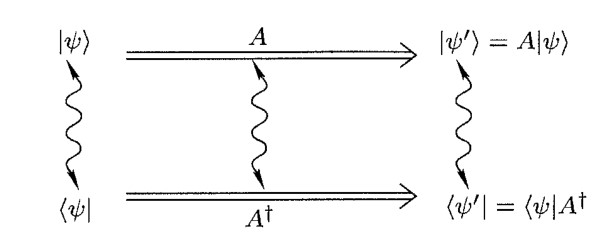
\includegraphics[width=0.9\textwidth]{figure/operation.jpg}
        \caption{左右矢空间算符与态的对应}
        \label{fig:measureoperation}
    \end{figure}
        \begin{remark}
            由于$\hat{A}^\dagger$只在左矢空间中作用,这样不方便的地方在于,我们讨论标量积$\langle\psi_i|\hat{A}^\dagger|\psi_j\rangle$的时候,我们只能理解为$\hat{A}^\dagger$作用于左矢$\langle\psi_i|$上再和$|\psi\rangle$做内积的形式。我们可以人为定义$\hat{A}^\dagger$对右矢空间地作用:
            \begin{equation}\label{equ2:2A}
                (\langle\psi_i|\hat{A}^\dagger)|\psi_j\rangle=\langle\psi_i|(\hat{A}^\dagger|\psi_j\rangle)
            \end{equation}
            上式的意思是,对于给定的右矢$\hat{A}^\dagger|\psi_j\rangle$,总可以和某一个左矢$\langle\psi_i|$形成内积。于是$\hat{A}^\dagger|\psi_j\rangle$是一个确定的内积,从而$\hat{A}^\dagger$是右矢空间的一个确定的算符。同理我们也可以类似的定义$\hat{A}$是左矢空间上一个确定的算符,这样定义的好处在于比较灵活的联络了对偶空间间的算符,从而简化了计算与理解。
        \end{remark}
    \subsection{投影算符}
    本节我们讨论一个量子力学非常常用的一个算符:投影算符。它的引入是基于完备线性空间上任意一个态矢量$|\psi\rangle$都能表示成空间上的一组规范正交基的$\{|\varphi_i\rangle\}$的线性组合,并且展开系数一定为态矢量$|\psi\rangle$到基矢量的投影,即:
    \begin{equation}
        |\psi\rangle=\sum_i\langle\varphi_i|\psi\rangle|\varphi_i\rangle
    \end{equation}
    
    由于$\langle\varphi_i|\psi\rangle$是一个数,因此我们可以将它与$|\varphi_i\rangle$交换位置,可以得到投影算符的定义:
    \begin{equation}
        |\psi\rangle=\sum_i|\varphi_i\rangle\langle\varphi_i|\psi\rangle=\Big(\sum_i|\varphi_i\rangle\langle\varphi_i|\Big)|\psi\rangle=\hat{P}|\psi\rangle
    \end{equation}
    
    如果$\{\varphi_i\}$是一个完备基,那么我们可以将上式看作一个恒等算符$\hat{I}$作用在$|\psi\rangle$上。投影算符的作用是对$|\psi\rangle$在规范正交基$\{\varphi_i\}$下进行投影和分解。
    
    投影算符的一个重要性质就是它的幂等性,即$\hat{P}^2=\hat{P}$:
    \begin{equation}
        \hat{P}^2=\sum_{i,j}|\varphi_i\rangle\langle\varphi_i|\varphi_j\rangle\langle\varphi_j|=\sum_{i,j}|\varphi_i\rangle\langle\varphi_j|\delta_{ij}=\sum_i|\varphi_i\rangle\langle\varphi_i|=\hat{P}
    \end{equation}
    
    \subsection{表象}
    在线性代数中,我们知道,如果我们需要具体的量化矢量的变换,我们可以利用建立坐标轴,利用一组数字来代表矢量与算符\footnote{也就是建立同构关系}。而建立坐标轴的过程也就是在线性空间中取一组基的过程。在量子力学中,我们称取一组基叫做取一个表象。假设$|\phi\rangle,|\psi\rangle$可以按照表象$Q$展开:
    \begin{align}
        \begin{split}
            |\phi\rangle=&\sum_i\langle\varphi_i|\phi\rangle|\varphi_i\rangle=\sum_i b_i|\varphi_i\rangle\\
            |\psi\rangle=&\sum_j\langle\varphi_j|\psi\rangle|\varphi_j\rangle=\sum_j c_j|\varphi_j\rangle
        \end{split}
    \end{align}
    
    假设$|\psi\rangle,|\phi\rangle$之间可以用算符$\hat{A}$联系:
    \begin{equation}
        |\phi\rangle=\hat{A}|\psi\rangle
    \end{equation}
    
    于是有:
    \begin{equation}
        \sum_i b_i|\varphi_i\rangle=\sum_j c_j\hat{A}|\varphi_j\rangle
    \end{equation}
    
    等式两边左乘一个$\langle\varphi_i|$,再利用$\langle\varphi_i|\varphi_j\rangle=\delta_{ij}$的性质,我们可以得到:
    \begin{equation}\label{equ2:2B}
        b_i=\sum_j\langle\varphi_i|\hat{A}|\varphi_j\rangle c_j=\sum_i A_{ij}c_j
    \end{equation}
    
    其中$A_{ij}=\langle\varphi_i|\hat{A}|\varphi_j\rangle$。我们得到了展开系数之间的关系,如果我们令展开系数为列向量的话,我们可以将式\ref{equ2:2B}表示成类似矩阵\footnote{这里说类似矩阵是因为矩阵仅仅针对有限维空间,而量子力学所在空间是无穷维的,因此我们可以类比的想}之间的关系了:
    \begin{equation}
        \begin{pmatrix}
            b_1\\
            b_2\\
            \vdots\\
            b_n\\
            \vdots
        \end{pmatrix}=
        \begin{pmatrix}
            A_{11} & A_{12} & \dots & A_{1n} & \dots\\
            \dots&\dots&\dots&\dots&\dots\\
            A_{m1}&A_{m2}& \dots &A_{mn}&\dots\\
            \dots&\dots&\dots&\dots&\dots
        \end{pmatrix}
        \begin{pmatrix}
             c_1\\
            c_2\\
            \vdots\\
            c_n\\
            \vdots
        \end{pmatrix}
    \end{equation}
    
    于是我们可以知道算符$\hat{A}$在表象Q中对应一个矩阵A,矩阵元为$A_{ij}$。
    
    \subsection{表象变换}
    下面我们讨论不同表象间的变换问题。在线性代数中我们已经知道线性空间中基的变换与过渡矩阵相联系相联系。特别的,在复线性空间中,如果两个基都是规范正交基,那么此时的基变换被称作幺正变换,其对应的过度矩阵Q满足关系:
    \begin{equation}
        Q^\dagger Q=QQ^\dagger=I
    \end{equation}
    
    迁移到量子力学的框架中,由于态空间也是一个复内积空间,同时对于某个表象,我们同样可以将每一个态表示成列向量的形式,因此可以想象,态空间$\mathscr{E}$中的变换也是满足幺正变换的,本节我们验证这个命题。
    
    假设态矢量$|\psi\rangle$可以用两种表象$|a_i\rangle,|b_i\rangle$展开,则有:
    \begin{align}
        \begin{split}
            |\psi\rangle=&\sum_i\langle a_i|\psi\rangle|a_i\rangle=\sum_i C_i^a|a_i\rangle\\
            |\psi\rangle=&\sum_j\langle b_j|\psi\rangle|b_j\rangle=\sum_j C_j^b|b_j\rangle
        \end{split}
    \end{align}
    
    两式联立,可得:
    \begin{equation}
        \sum_i C_i^a|a_i\rangle=\sum_j C_j^b|b_j\rangle
    \end{equation}
    
    等号两边左乘一个$\langle b_k|$,并且由于正交归一关系:$\langle b_k|b_j\rangle=\delta_{kj}$可得:
    \begin{equation}\label{equ2:2C}
        C_k^b=\sum_i C_i^a\langle b_k|a_i\rangle=\sum_i S_{ki}C_i^a
    \end{equation}
    
    其中:
    \begin{equation}
        S_{ki}=\langle b_k|a_i\rangle
    \end{equation}
    
    式\ref{equ2:2C}同样可以写成矩阵形式:
    \begin{equation}
        C^b=S C^a
    \end{equation}
    
    下面我们验证变换矩阵$S$是否是幺正的,我们的思路是通过向表象$\{|a_i\rangle\},\{|b_i\rangle\}$插入投影算符以构造矩阵元$S_{ij}=\langle b_i|a_j\rangle$:
    
    首先向表象$\{|a_i\rangle\}$的正交归一式子中插入投影算符:
    \begin{equation}
         \delta_{ij}=\langle a_i|a_j\rangle=\sum_k \langle a_i|b_k\rangle\langle b_k|a_j=\sum_k S_{ik}^*S_{kj}
    \end{equation}
 
    其矩阵形式为:
    \begin{equation}
        S^\dagger S=I
    \end{equation}
    
    同理,如果我们向表象$\{|b_i\rangle\}$的正交归一式子中插入投影算符,我们可以类似得到:
     \begin{equation}
        S S^\dagger=I
    \end{equation}

   随后我们讨论算符的幺正变换,即对于表象L和表象Q,算符$\hat{A}$对应的矩阵元形式分别为:$A_{ij}=\langle v_i|\hat{A}|v_j\rangle,A_{\alpha\beta}=\langle w_\alpha|\hat{A}|w_\beta\rangle$,如果表象L和表象Q的基底满足某个幺正变换,对应的矩阵用$U$来表示,则对应矩阵元的变换关系为:
   \begin{equation}
       \langle v_i|\hat{A}|v_j\rangle =\sum_\alpha\sum_\beta \langle v_i|w_\alpha\rangle\langle w_\alpha|\hat{A}|w_\beta\rangle\langle w_\beta|v_j\rangle=\sum_\alpha\sum_\beta U^\dagger_{i\alpha}A_{\alpha\beta}U_{\beta j}
   \end{equation}
   
   我们可以将其看作三个矩阵的相乘($A'=U^\dagger$),同理,我们可以采用相同的方法进行反表示:
   \begin{equation}
        \langle w_\alpha|\hat{A}|w_\beta\rangle=\sum_i\sum_j U_{\alpha i}A_{ij}U^\dagger_{j\beta}
   \end{equation}
   
   由上面的表述,我们可以很容易验证表现变换不改变内积$\langle\psi|\varphi\rangle$以及矩阵元的值$\langle\psi|\hat{A}|\varphi\rangle$。这与我们的物理图像相符。
\section{态空间中物理量的表征}
    \subsection{测量}
        \subsubsection{测量的基本性质}
        本节我们讨论如何表征态空间$\mathscr{E}$中的物理量。在日常生活\footnote{特指用经典力学分析的情况}中,如果想要知道一些宏观物理量,比如体系的位移、温度、压强,最朴素的获得方法就是通过一台对应的一起对待测体系进行测量,如光电门测量位移、温度计测温度、压强计测压强等。根据上面的经验,我们可以归纳出测量的大概定义:即将待测体系与一个满足经典力学规律的仪器相互作用后得到对应物理量的过程。
        
        当一个经典仪器作用到被观测的量子客体上的时候,我们称之为一次“操作”(operation)。我们的目的是要标志该客体状态一些可观测物理量的数值。这里分为两种情况:第一种情况是在做了第一次测量以后,仪器能够给出确定的度数,但是使用同样的仪器再测量第二次、第三次测量,给出的度数和第一次度数可能相等也可能不同,这种测量被称为第一类测量;第二种情况与第一类测量不同,在第一次测量以后,再用相同的仪器对同一客体做第二次测量、第三次测量时,仪器的读数总是百分百完全相同。第二类测量又被称为可预测的(predictable),是量子力学中"一次测量"的准确含义。换句话说,第二类测量给出的读数标志一个量子客体状态的一个力学量。
        
        我们可以这样理解:对于一个态的某一种力学量的测量,连续两次都给出同一数值,也就说测量以后态不发生改变。对于态空间$\mathscr{E}$中的某个态$|\psi\rangle$,如果我们想要进行物理量A的测量,同时测量结果为a,我们可以用本征方程来形容这个测量的过程:
        \begin{equation}
            \hat{A}|\psi\rangle=a|\psi\rangle
        \end{equation}
        
        自然的,我们称态$|\psi\rangle$为力学量$\hat{A}$的一个本征态,对应的数值称为它的一个本征值。特别的,如果一个本征值对应多个本征函数,则称本征值对应的本征函数是简并的;简并的本征函数的个数称为简并度;如果一个本征值对应一个本征函数,我们称该本征值对应的本征函数是非简并的。
        
        下面思考一个问题:之前引入波函数的时候,根据实际需要规定了单值、连续、有限三个性质,那么在这里我们将测量定义为了对应的算符,那么算符有什么限制呢?
        
        从上面的叙述中,我们知道测量与经典仪器的相互作用有关,为了得到更加普遍的结论,我们希望能够略去经典仪器本身的性质与限制(如精度,量程)。因此我们假设对于某一个量子客体的一个力学量A测量所得到的读数全体$\{a_n\}$应该穷尽所有的可能值;换句话说,态空间$\mathscr{E}$上的任意一个态能被力学量A对应的所有本征态线性表示,因此一定有关系:
        \begin{equation}
            |\psi\rangle=\sum_i c_i|\psi_i\rangle\xrightarrow{\hat{A}}\hat{A}|\psi\rangle=\sum_i c_ia_n|\psi_i\rangle
        \end{equation}
        
        需要说明的是,上面两式和测量时发生的塌缩是没有关系的,引入它们的本质是量子力学的态叠加原理。从物理上来讲,当许多个量子客体在相同的初始条件下被制备出来以后,人们对其逐一地进行力学量A地测量,原则上会得到不同的读数,我们自然希望知道不同读数之间有没有关联。在波函数公设中,我们了解到波函数的物理意义是有统计意义的,于是我们可以类似提出测量公设:
        \begin{definition}{测量公设}{measurement}
            对于物理量A,一定存在一个对应的测量算符$\hat{A}$,使得A的所有可取值都是$\hat{A}$本征方程的本征值集$\{a_i\}$
            \begin{equation}
                 \hat{A}|\psi_i\rangle=a_i|\psi_i\rangle
            \end{equation}
            并且其对应的本征态的集合$|\psi_i\rangle$构成态空间上的一组完备基,即:
            \begin{equation}
                |\psi\rangle=\sum_i c_i|\psi_i\rangle
            \end{equation}
            
            其中测量值为$a_i$的概率为:$|\langle \psi_i|\psi\rangle|^2$
        \end{definition}
        
        如果我们考虑简并态的话,假设测量值为$a_i$对应的简并度为$g_i$,那么测量到$a_i$的概率应该为塌缩到对应本征子空间本征函数的概率之和,即:$\sum_i^{g_i}|\langle\psi_{j=1}^{g_i}|\langle\psi_{i=1}^j|\psi\rangle^2$
        \subsubsection{测量的统计性质}
        值得一提的是,测量假设需要用到统计的思想进行诠释。从操作的层面上来讲,如果我们采用频率逼近的方式,即同时测量很多个同一个本征态N次,当$N\rightarrow \infty$时,我们知道测量物理量A的概率会收敛到某一个确定的值上:
        \begin{equation}
            \frac{N(a)}{N}\rightarrow P(a)
        \end{equation}
        
        在$|\psi\rangle$态中,我们定义$\langle A\rangle$为测量N次以后所得到测量值的平均值。根据定义,测量的平均值应该等于测量值的加权:
        \begin{equation}
            \langle \hat{A} \rangle=\frac{1}{N}\sum_n a_n N(a_n)
        \end{equation}
        
        当$N\rightarrow \infty$时,平均值趋于一个确定的值:
        \begin{equation}
             \langle \hat{A} \rangle=\sum_n a_n P(a_n)
        \end{equation}
        
        而根据公设$\ref{def:measurement}$,我们可以知道,如果对于简并本征态集$\{|\psi_n^i\rangle\}$ $P(a_n)$可以被表达为:
        \begin{equation}
            P(a_n)=\sum_{i=1}^{g_n}\langle\psi|\psi_n^i\rangle\langle \psi_n^i|\psi\rangle
        \end{equation}
        
        代入可得:
        \begin{equation}
             \langle \hat{A} \rangle=\sum_n a_n \Big(\sum_{i=1}^{g_n}\langle\psi|\psi_n^i\rangle\langle \psi_n^i|\psi\rangle\Big)
        \end{equation}
        
        代入本征方程:$\hat{A}|\psi_n^i\rangle=a_n|\psi_n^i\rangle$,可以得到:
        \begin{equation}
            \langle \hat{A} \rangle=\sum_n  \sum_{i=1}^{g_n}\langle\psi|\hat{A}|\psi_n^i\rangle\langle \psi_n^i|\psi\rangle
        \end{equation}
        
        由于本征态集$\{|\psi_n^i\rangle\}$是一个正交归一集,于是一定有封闭性关系:
        \begin{equation}
            \sum_n\sum_{i=1}^{g_n}|\psi_n^i\rangle\langle \psi_n^i|=\hat{I}
        \end{equation}
        
        于是可以得到:
        \begin{equation}
            \langle \hat{A}\rangle=\langle\psi|\hat{A}|\psi\rangle
        \end{equation}
        
        我们由此得到了测量值平均值的表达式,这有助于我们判断态矢量的性质。
        
        测量的标准除了准确度以外还有精确度,前者我们往往使用平均值(或称为期望)描述,而后者我们往往使用标准差描述。在测量中,由于算符的不对易,导致物理量的测量常常会相互干扰,因此我们常常考虑多个物理量标准差之间的关系\footnote{这里的内容要用到下一节中测量算符是厄密算符的性质,可以跳过想看下一节再回过头来理解}。首先我们考虑对$|\psi\rangle$态进行力学量A的测量所产生的标准差$\sigma_A^2$:
        \begin{align}
            \begin{split}
             \sigma_A^2=&\left\langle(\hat{A}-\langle\hat{A}\rangle)^2 \right\rangle\\
                =& \langle\psi|(\hat{A}-\langle\hat{A}\rangle)^2|\psi\rangle\\
                =&\langle(\hat{A}-\langle\hat{A})\psi|(\hat{A}-\langle\hat{A})\rangle|\psi\rangle\\
                =&\langle f|f\rangle
            \end{split}
        \end{align}
            
       其中$|f\rangle=(\hat{A}-\langle\hat{A})\rangle|\psi\rangle$。同样的方法,对$|\psi\rangle$态进行力学量B的测量所产生的标准差$\sigma_B^2$为:
       \begin{equation}
           \sigma_B^2=\langle g|g\rangle
       \end{equation}
       
       其中:$|g\rangle=(\hat{B}-\langle\hat{B}\rangle)|\phi\rangle$。
       
       我们通过Cauchy-Schwarz不等式,可以建立两个力学量标准差的关系:
       \begin{equation}
           \sigma_A^2\sigma_B^2=\langle f|f\rangle\langle g|g\rangle\geq (\langle f|g\rangle)^2
        \end{equation}

        随后对$\langle f|g\rangle$进行估计,由于这个标量积的结果一定是个复数,而对于任意的复数$z$,一定有以下缩放不等式:
        \begin{equation}
            z=Rez+Imz\geq Imz=\frac{1}{2i}(z-z^*)
        \end{equation}
        
        令$z=\langle f|g\rangle$,则$z^*=\langle g|f\rangle$,代入可得:
        \begin{equation}
            \langle f|g\rangle \geq \frac{1}{2i}(\langle f|g\rangle-\langle g|f\rangle)
        \end{equation}
        
        根据$\langle f|g\rangle$的定义,我们可以得到:
        \begin{align}
            \begin{split}
                \langle f|g\rangle=&\langle\psi|(\hat{A}-\langle\hat{A}\rangle)(\hat{B}-\langle\hat{B}\rangle)|\phi\rangle\\
                =&\langle\psi|(\hat{A}\hat{B}-\langle\hat{A}\rangle\hat{B}-\hat{A}\langle\hat{B}\rangle+\langle\hat{A}\rangle\langle\hat{B}\rangle)|\phi\rangle
            \end{split}
        \end{align}
        
        同理,对于$\langle g|f\rangle$,有\footnote{这里的第二个等号利用了厄米算符矩阵元的定义:$\langle\phi|\hat{A}|\psi\rangle=\langle\psi|\hat{A}|\phi\rangle$,详细证明可以见下一节}:
        \begin{align}
            \begin{split}
                \langle g|f\rangle=&\langle\phi|(\hat{B}\hat{A}-\langle\hat{A}\rangle\hat{B}-\hat{A}\langle\hat{B}\rangle+\langle\hat{A}\rangle\langle\hat{B}\rangle)|\psi\rangle\\
                =&\langle\psi|(\hat{B}\hat{A}-\langle\hat{A}\rangle\hat{B}-\hat{A}\langle\hat{B}\rangle+\langle\hat{A}\rangle\langle\hat{B}\rangle)|\phi\rangle
            \end{split}
        \end{align}
            
        于是代入上述所有式子可以得到一个重要的不等式:
        \begin{equation}
            \sigma_A^2\sigma_B^2\geq \Big(\frac{1}{2i}\langle [\hat{A},\hat{B}]\rangle\Big)^2
        \end{equation}
        
        上式被称为广义的不确定原理,对于每一对不对易的力学量测量算符,都存在这样类似的测不准原理\footnote{关于不对易的力学量测量算符的性质,将在\ref{subsection:ESCO}节中给予详细阐释}。特别的当$\hat{A}=\hat{x},\hat{B}=\hat{p_x}$时,我们知道$[\hat{x},\hat{p_x}]=i\hbar$,代入上式,可以得到$\sigma_x\sigma_{p_x}\geq\frac{\hbar}{4}$。
        
        \begin{remark}
            从上面的表述可以看到,测不准原理并不是量子力学新的假设,而是实验的自然推断,也是量子力学具有统计性质的根源之一。
        \end{remark}
    \subsection{测量算符}
        本节我们继续探讨测量算符具有什么性质。从测量结果的角度来看,对任意一个可观测物理量的测量结果都应该为实数。这一点体现为:对于$\hat{A}$的本征态来说,我们要保证其本征值为实数;对于一般的态$|\psi\rangle$,虽然它的测量结果各有不同,但是由于所有的测量结果都应为实数,因此平均值$\langle\psi|\hat{A}|\psi\rangle$一定为实数,因此$\langle\psi|\hat{A}|\psi\rangle$一定等于其共轭\footnote{这里利用到了标量积的性质:
        \begin{equation*}
            (\langle\psi|\hat{A}|\phi\rangle)^*=( (\langle\psi|\hat{A}\phi\rangle)^*=\langle\hat{A}\phi|\psi\rangle=\langle\psi|\hat{A}^\dagger|\phi\rangle
        \end{equation*}}:
        \begin{equation}
            \langle \psi|\hat{A}|\psi\rangle=(\langle\psi|\hat{A}|\psi\rangle)^*=\langle\psi|\hat{A}^\dagger|\psi\rangle
        \end{equation}
        
        因此测量算符一定满足$\hat{A}=\hat{A}^\dagger$,我们称$\hat{A}$是厄米算符。因此有关测量算符的假设就与厄米算符有关:
        \begin{definition}{算符公设Ⅱ}{measurement2}
            测量算符一定是一个厄米算符。
        \end{definition}
        
        厄米算符还有其它良好的性质。假设$|\phi_1\rangle,|\phi_2\rangle$是测量算符$\hat{A}$不同本征值对应的本征态,即有本征方程:
        \begin{align}
            \begin{split}
                \hat{A}|\phi_1\rangle=a_1|\phi_1\rangle\\
                \hat{A}|\phi_2\rangle=a_2|\phi_2\rangle
            \end{split}
        \end{align}
        
        考虑标量积$\langle\phi_1|\hat{A}|\phi_2$,结合本征方程,可以得到:
        \begin{equation}
            a_1\langle\phi_1|\phi_2\rangle=\langle\phi_1|\hat{A}|\phi_2=a_2\langle\phi_1|\phi_2\rangle
        \end{equation}
        
        由于$a_1\ne a_2$,因此$\langle\phi_1|\phi_2\rangle=0$,也即:厄米算符不同本征值对应的本征态相互正交。这个性质非常重要,对于同一本征值的本征态,我们一定可以通过Gram-Schimdt正交化获得正交归一的本征态集。综上所述,如果算符是Hermitian的,我们一定可以找到一组正交归一的完备基。
    \subsection{可对易观察算符的完全集合(ESCO)}\label{subsection:ESCO}
    本节我们考虑两个对易的观察算符所具有的性质。首先从两个简单的性质出发:
    \begin{theorem}{性质1}{property1}
    如果$[\hat{A},\hat{B}]=0$,则$\hat{A}$的所有本征子空间在$\hat{B}$的作用下不变,即:对于$\hat{A}$的任意本征值$a_n$所对应的本征子空间$\mathscr{E}_{a_n}$,如果$|\psi\rangle\in\mathscr{E}_{a_n}$,则$\hat{B}|\psi\rangle\in\mathscr{E}_{a_n}$
    \end{theorem}
    \begin{proof}
    假设$|\psi\rangle$是算符$\hat{A}$的本征态,本征值为a,则根据对易关系,$\hat{A}\hat{B}=\hat{B}\hat{A}$,有:
    \begin{equation}
        \hat{A}(\hat{B}|\psi\rangle)=\hat{B}\hat{A}|\psi\rangle=a(\hat{B}|\psi\rangle
    \end{equation}
    
    由上式,我们知道$\hat{B}|\psi\rangle$也满足$\hat{A}$的本征方程,故证得
    \end{proof}
    \begin{theorem}{性质2}{property2}
        如果$[\hat{A},\hat{B}]=0$,并且$|\psi_1\rangle,|\psi_2\rangle$是算符$\hat{A}$的两个不同的本征态,并且属于不同的本征值,则$\langle\psi_1|\hat{B}|\psi_2\rangle=0$
    \end{theorem}
    \begin{proof}
    由定理\ref{thm:property1}可得,当$[\hat{A},\hat{B}]$对易的时候,$\hat{B}|\psi_2\rangle\in \mathscr{E}_{a_2}$。根据厄米算符的性质,不同本征值对应的本征态是相互正交的,因此$\langle\psi_1|\hat{B}|\psi_2\rangle=0$
    \end{proof}
    
    根据性质1、性质2,我们可以得到非常重要的性质3:
    \begin{theorem}{性质3}{property3}
        如果观察算符满足$[\hat{A},\hat{B}]=0$,则它们共同本征态构成态空间$\mathscr{E}$上的一组完备正交归一基。
    \end{theorem}
    \begin{proof}
        证明性质3,本质上就是证明一定存在一组规范正交基组$\{v_n^i\}$,使得$\hat{A},\hat{B}$在这组基对应的矩阵是对角矩阵。假设$\{|u_n^i\rangle\}$是$\hat{A}$的一组本征态,则一定满足本征方程:
        \begin{equation}
            \hat{A}|u_n^i\rangle=a_n|u_n^i\rangle,i=1,2\dots,g_n
        \end{equation}
        
        其外,基一定满足正交归一关系:
        \begin{equation}
            \langle u_n^i|u_{n'}^{i'}\rangle=\delta_{ii'}\delta_{nn'}
        \end{equation}
        
        可以看到,此时$\hat{A}$在$\{|u_n^i\rangle\}$下的矩阵是对焦矩阵,那么$\hat{B}$在$\{|u_n^i\rangle\}$下的矩阵形式是怎么样的呢?根据性质2,我们知道B矩阵的矩阵元满足$\langle u_n^i|\hat{B}|u_n^{i'}\rangle=0$,由此可以看出B的形式应该是一个分块对角矩阵,每一个子块是一个$g_n\times g_n$的矩阵(如图\ref{fig:multiblock})
       
        我们分情况讨论。如果$\{|u_n^i\rangle\}$是非简并的,即$g_n=1,n=1,2,\dots$,那么B矩阵就是对角矩阵,此时性质3已经成立;如果如果$\{|u_n^i\rangle\}$是简并的,即$\exists n,g_n\ne1$,此时可以发现$\{|u_n^i\rangle\}$不是$\hat{B}$的本征态。由于$\hat{A}$存在本征方程,也就是说,我们可以使用$\hat{A}$的本征子空间表示态空间$\mathscr{E}$:
        \begin{equation}
            \mathscr{E}=\mathscr{E}_{a_1}\oplus \mathscr{E}_{a_2}\oplus\dots\oplus \mathscr{E}_{a_n}\oplus\dots
        \end{equation}
        
        于是,本征子空间中的任意一组正交归一基都能让A称为对角矩阵。对于B矩阵,由于$\hat{B}$是Hermitian的,因此B矩阵的子块也一定是Hermitian的。根据线性代数的知识,厄米矩阵一定是可以对角化的,因此一定存在正交归一基$\{|v_n^i\rangle\}$,使得:
        \begin{equation}
            \langle v_n^i|\hat{B}|v_n^j\rangle=\delta_{ij}
        \end{equation}
        
        由此简并态的情况也满足性质3,证毕。
        
         \begin{figure}[H]
            \centering
            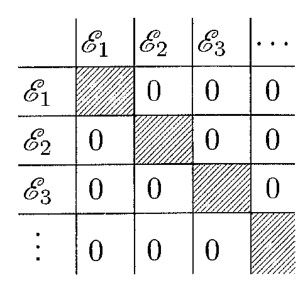
\includegraphics{figure/multiblock.jpg}
            \caption{B矩阵在基$\{|u_n^i\rangle\}$是一个分块对角矩阵}
            \label{fig:multiblock}
        \end{figure}
        
    \end{proof}

性质3提供了对易的观察算符的一个非常好的性质,但是其中有一个细节值得揣摩:能将算符$\hat{B}$对角化后的新的本征态是$\hat{A}$同一本征值下的本征态吗?答案是不一定是。因为在上面的证明中我们仅仅只能保证新的基的存在性,而不能保证新的基与变换前的基与本征值一一对应。这一点看似性质不是很好,但是实际上对于简并情况来说,如果我们测量物理量A,结果为$a_n$,可能存在两个本征态$|\psi_1\rangle,|\psi_2\rangle$满足本征方程,这样从测量的角度上来看我们并不能分辨这两个本征态。此时我们可以通过测量另一个与$\hat{A}$对易的物理量B来分辨这两个状态;换句话说,如果存在一组本征值组$\{a_n,b_p\}$对应唯一的一个态矢量,我们就能够通过测量完全确定一个态;如果本征值组$\{a_n,b_p\}$仍然不能对应唯一一个态矢量,那么我们就引入与$\hat{A},\hat{B}$对易的物理量C,如果存在一组本征值组$\{a_n,b_p,c_r\}$对应唯一一个共同的本征态,那么就可以通过测量完全确定一个态;如果不能,继续引入新的对易算符$\dots$\footnote{其实可以看出,引入对易算符并通过测量的本征值描述态本质上就是回归了经典力学描述状态的方法,我们可以将测量的本征值看作描述状态的自由度}。由此,我们引出了CSCO的概念:
\begin{definition}{CSCO}{CSCO}
    如果测量算符$\hat{A},\hat{B},\hat{C}\dots$相互对易,并且一定存在测量的本征值组$\{a_n,b_p,c_r\}$确定唯一的一个共同本征态,我们将果测量算符$\hat{A},\hat{B},\hat{C}\dots$的集合称为可对易观察算符的完全集合,简写为CSCO。
\end{definition}

对于CSCO,还有几点注意:
\begin{enumerate}
    \item 通常我们只考虑最小的CSCO,如果$\hat{A},\hat{B}$已经构成了CSCO,在一般情况下我们不会考虑继续加一个新的算符$\hat{C}$;
    \item 由于一组本征值组确定唯一一个本征态,因此我们可以将本征态简记为本征值组的形式,如:$|a_n,b_p,c_r\rangle$;
    \item 对于一个给定的态空间,CSCO可能不止一组。
\end{enumerate}

    CSCO还有一个值得讨论的点,就是多个算符在操作上是如何测量的。首先,由于测量以后,在短时间内会发生态的塌缩,但是态在其它时候都是遵循Schrodinger方程的演化\footnote{详细讨论可以见\ref{section2:evolution}节}。因此算符测量见的间隔不能太长;此外测量的先后顺序会不会影响最后的结果呢?答案显然是否定的,在这里我们讨论一种简单的情况,即$\hat{A},\hat{B}$构成CSCO,我们设共同本征态为$|a_n,b_p\rangle$,于是对于态空间上的任意一个态$|\psi\rangle$,我们总是可以表示为:
    \begin{equation}
        |\psi\rangle=\sum_{n,p}c_{n,p}|a_n,b_p\rangle
    \end{equation}
    
    于是根据测量公设,第一次测量物理量A对应的测量值为$a_n$的概率为:
    \begin{equation}
        P(a_n)=\sum_p |c_{n,p}|^2
    \end{equation}
    
    第一次测量后的态从$|\psi\rangle$变为$|\psi'\rangle$\footnote{公式里的n是一个定值而不是变量,可以将其看作投影算符对$|\psi\rangle$的作用,使之从高维空间的矢量压缩成了低维空间的矢量。}:
    \begin{equation}
        |\psi'\rangle=\sum_p c_{n,p}|a_n,b_p\rangle\cdot \frac{1}{\sqrt{\sum_p|c_{n,p}|^2}}
    \end{equation}
    
    其中乘积的第二项是考虑到了态的归一化。此时我们可以获得在第一次测量物理量A的结果为$a_n$的前提下,第二次测量物理量B的结果为$b_p$的条件概率为:
    \begin{equation}
        P(b_p|a_n)=\frac{|c_{n,p}|^2}{\sqrt{\sum_p|c_{n,p}|^2}}
    \end{equation}
    
    于是,根据概率公式,我们可以得到测量结果为$a_n,b_p$的概率为:
    \begin{equation}
        P(a_n,b_p)=P(a_n)P(b_p|a_n)=|c_{n,p}|^2
    \end{equation}
    
    同理,对于先测量物理量B后测量物理量A的情况,我们也能得到同样的结果,因此无论测量是按照何种顺序进行的,物理上的结果都是一样的。但是对于不对易的算符来说就不同了。举一个简单的例子:假设态空间是一个二维的矢量空间,$|u_1\rangle,|u_2\rangle$是$\hat{A}$本征值为$a_1,a_2$的本征态,$|v_1\rangle,|v_2\rangle$是本征值为$b_1,b_2$的本征态。有图可知,$\hat{A},\hat{B}$没有共同的本征态,因此它们是不对易的。现在考虑对态空间中的任意态$|\psi\rangle$分别进行以下两种测量:
    \begin{align}
        \begin{split}
            a_1,b_2:|\psi\rangle\rightarrow|u_1\rangle\rightarrow|v_2\rangle\\
            b_2,a_1:|\psi\rangle\rightarrow|v_2\rangle\rightarrow|u_1\rangle
        \end{split}
    \end{align}

    我们可以看见两种路径都是测量出$a_1,b_2$的结果,但是末态不同,我们考虑两种路径测量的概率:
    \begin{align}
        \begin{split}
            P(a_1,b_2)=&|OH_1|^2\cdot|OK_2|^2\\
            P(b_2,a_1)=&|OH_2|^2\cdot|OK_1|^2
        \end{split}
    \end{align}
    
    显然$P(a_1,b_2)\ne P(b_2,a_1)$。因此不对易的算符是不能同时测量的,因为第二次的测量会失去第一次测量所得到的信息,因为$|v_2\rangle$不是$\hat{A}$的本征态。
    \begin{figure}[H]
        \centering
        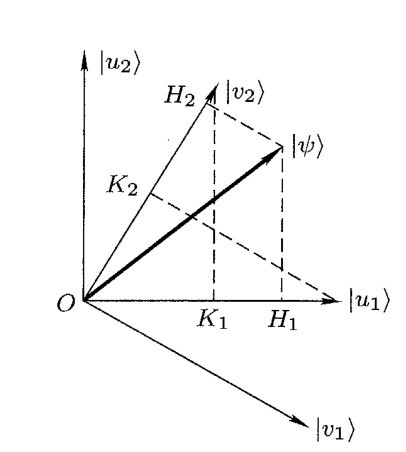
\includegraphics{figure/paradox.jpg}
        \caption{不对易算符不能同时测量}
        \label{fig:noncommuting}
    \end{figure}
\section{态的演化}\label{section2:evolution}
    \begin{definition}{Schrodinger方程公设}{Schrodingerequ}
        态$|\psi(t)\rangle$的演化遵循Schrodinger方程:
        \begin{equation}
            i\hbar\frac{d|\psi(t)\rangle}{dt}=\hat{H}|\psi(t)\rangle
        \end{equation}
        
        其中$\hat{H}$表示与体系能量有关的观察算符,我们称之为Hamiltonian。由于我们观察到这个方程式关于t的一阶微分方程,因此我们只要知道初始条件$|\psi(t_0)\rangle$,状态后续的演化就被唯一的确定
    \end{definition}
    
    本节我们主要从Schrodinger方程出发探讨几个方程的一般性质。
    \subsection{概率守恒}
    本节讨论态的一些统计限制。首先,随着Schrodinger方程的演化,态必须保证还在态空间中,也就是说,需要保证态矢量的归一化不随演化而改变,在数学上我们要证明态的模方$\langle\psi(t)|\psi(t)\rangle$不随时间而改变:
    \begin{equation}\label{equ:D}
        \frac{d}{dt}\langle\psi(t)|\psi(t)\rangle=\frac{d}{dt}\langle\psi(t)|\Big]|\psi(t)\rangle+\langle\psi(t)|\Big[\frac{d}{dt}|\psi(t)\rangle\Big]
    \end{equation}
    
    根据Schrodinger方程,我们可以得到左矢与右矢的导数的表达式:
    \begin{align}\label{equ2:E}
        \begin{split}
            \frac{d|\psi(t)\rangle}{dt}=&\frac{1}{i\hbar}\hat{H}|\psi(t)\rangle\\
            \frac{d\langle\psi(t)|}{dt}=&-\frac{1}{i\hbar}\langle\psi(t)|\hat{H}^\dagger=-\frac{1}{i\hbar}\langle\psi(t)|\hat{H}
        \end{split}
    \end{align}
    
    代入\ref{equ:D}式,可得:
    \begin{equation}
        \frac{d}{dt}\langle\psi(t)|\psi(t)\rangle=0
    \end{equation}
    
    由此我们知道态矢量的归一化不随着演化的改变而改变。事实上,这是一种全空间上的概率守恒;根据电磁学的知识,我们知道一种全局守恒必定对应一种局域守恒。所谓局域守恒,就是对于空间上的任意一个部分,单位时间内“流出”的物理量一定与单位时间内“流入”的物理量相同,其数学形式表现为下列的连续性方程:
    \begin{equation}
        \frac{\partial}{\partial t}\rho(r,t)+\nabla \cdot \Vec{J}=0
    \end{equation}
    
    其中$\rho$是局域空间的密度,$\Vec{J}$被称为该物理量对应的“流”。下面我们证明我们可以从Schrodinger方程推出连续性方程。
    
    由于密度一般来说是时空量,因此我们采用$|r\rangle$表象上的Schrodinger方程较为合适:
    \begin{equation}
        i\hbar\frac{\partial}{\partial t}\psi(r,t)=\Big(\frac{\hat{p}^2}{2m}\nabla^2+V(r,t)\Big)\psi(r,t)
    \end{equation}
    
    其共轭形式为:
    \begin{equation}
        -i\hbar\frac{\partial}{\partial t}\psi^*(r,t)=\Big(\frac{\hat{p}^2}{2m}\nabla^2+V(r,t)\Big)\psi^*(r,t)
    \end{equation}
    
    由于两式右边只有$V(r,t)$有关项是没有偏微分的,因此我们将两式联立消去方程的该部分,可得:
    \begin{align}
        \begin{split}
            i\hbar\Big\{\psi^*(r,t)\frac{\partial}{\partial t}\psi(r,t)+\psi^*(r,t)\frac{\partial}{\partial t}\psi(r,t)\Big\}\\
            =\frac{\hbar^2}{2m}\Big(\nabla^2\psi(r,t)\psi^*(r,t)-\nabla^2\psi^*(r,t)\psi(r,t)\Big)
        \end{split}
    \end{align}
    
    可以看到,等号左边可以根据全微分的计算得到结果为:$i\hbar\frac{\partial}{\partial t}(\psi(r,t)\psi^*(r,t))$,将系数除到等号右边进行化简可以得到:
    \begin{equation}
        i\hbar\frac{\partial}{\partial t}(\psi(r,t)\psi^*(r,t))=\frac{\hbar^2}{2m}\Big(\nabla^2\psi(r,t)\psi^*(r,t)-\nabla^2\psi^*(r,t)\psi(r,t)\Big)
    \end{equation}
    
    我们对等号右侧的式子通过加一项再减一项$\nabla\psi\nabla\psi^*$的方法,可以将右侧凑成一个式子的梯度,于是Schrodinger方程可以写成以下形式:
    \begin{equation}
        i\hbar\frac{\partial}{\partial t}(\psi(r,t)\psi^*(r,t))+\frac{i\hbar}{2m}\nabla[\nabla\psi(r,t)\psi^*(r,t)-\nabla\psi^*(r,t)\psi(r,t)]=0
    \end{equation}
    
    我们定义$\rho=\psi^*\psi$,$\Vec{J}=\frac{i\hbar}{2m}\nabla\psi(r,t)\psi^*(r,t)-\nabla\psi^*(r,t)\psi(r,t)$,就可以将Schrodinger方程转换为连续性方程。我们称此时的$\Vec{J}$为几率流。这个概念在诸如散射问题中有重要的作用。
    \subsection{可观测物理量的演化}\label{subsection:evolutionforoperator}
        在之前的章节中我们已经了解到了可观测物理量平均值满足$\langle\psi(t)|\hat{A}|\psi(t)\rangle$。可以看到,可观测物理量的平均值一方面和态有关,一方面与算符$\hat{A}$有关,而两者都有可能随时间发生变化,因此平均值随时间的演化对于描述算符的演化有重要作用,下面我们详细探讨一下:
        \begin{align}
            \begin{split}
                \frac{d\langle\hat{A}\rangle}{dt}=&\frac{d}{dt}\langle\psi(t)|\hat{A}|\psi(t)\rangle\\
                =&[\frac{d}{dt}\langle\psi(t)|]\hat{A}|\psi(t)\rangle+\langle\psi(t)|\frac{\partial\hat{A}}{\partial t}|\psi(t)\rangle+\langle\psi(t)|\hat{A}|[\frac{d}{dt}|\psi(t)]\\
            \end{split}
        \end{align}
        
        代入式\eqref{equ2:E},可以得到:
        \begin{equation}\label{equ2:evolutionforoperator}
            \frac{d\langle\hat{A}\rangle}{dt}= \langle\frac{\partial\hat{A}}{\partial t}\rangle+\frac{1}{i\hbar}\langle[\hat{A},\hat{H}]\rangle
        \end{equation}
        
        观察该式,我们发现它和经典力学中的Hamilton原理相似,不同的是经典力学中等式右侧第二项是泊松括号,而在量子力学中却变为了对易子。因此经典力学中的泊松括号和量子力学中的对易子是由对应关系的,这个关系最早由Dirac发现,我们将其称为正则量子化,在下一节中,我们将会阐述正则量子化的内容。
        
        \subsection{保守系与定态}
        如果$\hat{H}$不含时间,我们称体系是一个保守系。在经典力学中,如果体系是一个保守系,那么体系的能量守恒,也即能量是一个运动常量。本节我们讨论在量子力学框架下保守系具有的性质。
        
        假设$\hat{H}$满足以下本征方程:
        \begin{equation}
            \hat{H}|\varphi_{n,\tau}\rangle=E_n|\varphi_{n,\tau}\rangle
        \end{equation}
        
        于是,任意时刻t上的态都可以表示为本征态的线性组合:
        \begin{equation}
            |\psi(t)\rangle=\sum_{n,\tau}c_{n,\tau}(t)|\varphi_{n,\tau}\rangle
        \end{equation}
        
        代入Schrodinger方程,可以得到:
        \begin{align}
            \begin{split}
                i\hbar\frac{d}{dt}|\psi(t)\rangle=&\hat{H}|\psi(t)\rangle\\
                =&\hat{H}\Big(\sum_{n,\tau}c_{n,\tau}(t)|\varphi_{n,\tau}\rangle\Big)\\
                =&\sum_{n,\tau}c_{n,\tau}(t)E_n|\varphi_{n,\tau}\rangle
            \end{split}
        \end{align}
        
        用$\langle\varphi_{n,\tau}|$作用于上式,可以得到:
        \begin{align}
            \begin{split}
                i\hbar\frac{d}{dt}\langle \varphi_{n,\tau}|\psi(t)\rangle=&c_{n,\tau}E_n\\
                \Rightarrow i\hbar\frac{dc_{n,\tau}}{dt}=&c_{n,\tau}E_n
            \end{split}
        \end{align}
        
        这是一个简单微分方程,结果为:
        \begin{equation}
            c_{n,\tau}(t)=c_{n,\tau}(t_0)e^{-\frac{iE_n(t-t_0)}{\hbar}}
        \end{equation}
        
        则任意时刻的态$|\psi(t)\rangle$可以表示为:
        \begin{equation}
            |\psi(t)\rangle=\sum_{n,\tau}c_{n,\tau}(t_0)e^{-\frac{iE_n(t-t_0)}{\hbar}}|\varphi_{n,\tau}\rangle
        \end{equation}
        
        我们也可以将其拓展到连续基的情况:
        \begin{equation}
            |\psi(t)\rangle=\sum_{\tau}\int dE c_{E,\tau}(t_0)e^{-\frac{iE_n(t-t_0)}{\hbar}}|\varphi_{E,\tau}\rangle
        \end{equation}
        
        特别的,如果$|\psi(t_0)\rangle$也是$\hat{H}$的本征态,那么:
        \begin{equation}
            |\psi(t_0)\rangle =\sum_{n,\tau}c_{n,\tau}(t_0)|\varphi_{n,\tau}\rangle
        \end{equation}
        
        于是任意时刻的态可以表示为:
        \begin{equation}
            |\psi(t)\rangle=\sum_{n,\tau}c_{n,\tau}(t_0)e^{-\frac{iE_n(t-t_0)}{\hbar}}|\varphi_{n,\tau}\rangle=e^{-\frac{iE_n(t-t_0)}{\hbar}}|\psi(t_0)\rangle
        \end{equation}
        
        可以发现任意时刻的态与$t_0$时刻的态相比仅仅多了一个总的相位因子,根据上文的讨论,我们知道两个态的物理性质完全相同,即处在$\hat{H}$的本征态的所有可观测物理量的取值都不随时间变化,因此我们称之为定态。这是后续我们处理问题的立足点。
        
    %能量-时间不确定关系+光谱带宽    
\section{$|r\rangle$和$|p\rangle$表象}
    本节介绍常用的两个表象:$|r\rangle$和$|p\rangle$表象,用来复习第二章的主要脉络,同时这两个表象与经典力学的联系十分紧密,我们可以在后文看到一些有趣的结论
    \subsection{基的基本性质}
    通过扩充态空间$\mathscr{E}$,使得在实际操作上可以取所谓的连续基$\{\omega_\alpha\}$。下面介绍两个典型的连续基,一个是与$r$有关的$\delta$函数,一个是平面波函数,我们分别用$|r_0\rangle,|p_0\rangle$表示:
    \begin{align}
        \begin{split}
            |r_0\rangle=&\delta(r-r_0)=\xi_{r_0}(r)\\
            |p_0\rangle=&(2\pi\hbar)^{-\frac{3}{2}}\exp{\frac{ip_0\cdot r}{\hbar}}=v_{p_0}(r)
        \end{split}
    \end{align}
    
    虽然这两组基不在态空间内,但是态空间内的所有态都可以用它们表示。因此从这两个连续基出发,定义两种表象$|r\rangle,|p\rangle$。前者由x,y,z三个连续指标描述,后者由$p_x,p_y,p_z$三个连续指标描述。下面验证两组基的基本性质。首先根据态空间上标量积的定义,容易验证:
    \begin{align}
        \begin{split}
            \langle r_0|r_0'\rangle=&\int d^3r\xi^*_{r_0}(r)\xi_{r_0'}(r)=\delta(r_0-r_0')\\
            \langle p_0|p_0\rangle=&\int d^3p v^*_{p_0}(r)v_{p_0'}(r)=\delta(p_0-p_0')
        \end{split}
    \end{align}
    
    因此两种表象都是正交归一的,同时它们也满足封闭性:
    \begin{align}
        \begin{split}
            \int d^3 r_0|r_0\rangle\langle r_0|=1\\
            \int d^3 p_0 |p_0\rangle\langle p_0|=1
        \end{split}
    \end{align}
    
    将投影算符作用到态空间上的态$|\psi\rangle$上,可以得到:
    \begin{align}
        \begin{split}
            |\psi\rangle=&\int d^3 r_0|r_0\rangle\langle r_0|\psi\rangle\\
            |\psi\rangle=&\int d^3 p_0|p_0\rangle\langle p_0|\psi\rangle
        \end{split}
    \end{align}
    
    其中展开系数可以这样表示:
    \begin{align}
        \begin{split}
            \langle r_0|\psi\rangle=&\int d^3 r\xi_{r_0}^*(r)\psi(r)=\psi(r_0)\\
            \langle p_0|\psi\rangle =& \int d^3p v_{p_0}^*(r)\psi(r)=\overline{\psi(p_0)}
        \end{split}
    \end{align}
    
    因此,波函数$\psi(r_0)$代表态在表象$|r\rangle$上对应$|r_0\rangle$的坐标。同理,$\overline{\psi(p_0)}$也有类似的解释。
    \subsection{$|r\rangle$到$|p\rangle$的表象变换}
        本节主要讨论$\psi(r)$与$\overline{\psi(p)}$的关系,首先考虑标量积$\langle r|p\rangle$:
        \begin{equation}
            \langle r|p\rangle=v_p(r)=(2\pi\hbar)^{-\frac{3}{2}}\exp{\frac{ip\cdot r}{\hbar}}
        \end{equation}
        
        插入封闭关系式可以得到:
        \begin{align}
            \begin{split}
                \psi(r)=\langle r|\psi\rangle=&\int d^3 p\langle|p\rangle\langle p|\psi\rangle =(2\pi\hbar)^{\frac{3}{2}}\int d^3 p\exp{\frac{ip\cdot r}{\hbar}}\overline{\psi(p)}\\
                \overline{\psi(p)}=\langle p|\psi\rangle=&\int d^3 r\langle p|r\rangle\langle r|\psi\rangle=(2\pi\hbar)^{-\frac{3}{2}}\int d^3r\exp{\frac{ip\cdot\psi(r) r}{\hbar}}
            \end{split}
        \end{align}
        
        可以明显发现,两者满足Fourier变换。下面我们讨论可观测量的表象变换,考虑算符$\hat{A}$在$|r\rangle$表象下的矩阵元$\langle r'|\hat{A}|r\rangle$,我们通过插入两个封闭关系构造$\hat{A}$在$|p\rangle$表象下的矩阵元$\langle p'|\hat{A}|p\rangle$:
        \begin{align}
            \begin{split}
                \langle r'|\hat{A}|r\rangle=&\int d^3p'\langle r'|p'\rangle\int d^3p\langle p'|\hat{A}|p\rangle\langle p|r\rangle
                \\=&(2\pi\hbar)^{-3}\int d^3p'\langle r'|p'\rangle\int d^3p \exp{\frac{i(p'-p)\cdot r}{\hbar}}\langle p'|\hat{A}|p\rangle
            \end{split}
        \end{align}
    \subsection{观察算符$\hat{R}$和$\hat{P}$}
        本节我们讨论观察算符$\hat{R}$和$\hat{P}$的性质,我们假设态空间上存在与x方向有关的变换:
        \begin{equation}
            |\psi'\rangle=\hat{X}|\psi\rangle
        \end{equation}
        
        在$|r\rangle$表象下,根据测量算符的性质,我们知道一定有关系:
        \begin{equation}
            \langle r|\psi'\rangle=\langle r|\hat{X}|\psi\rangle= x\langle r|\psi\rangle
        \end{equation}
        
        同理:
        \begin{align}
            \begin{split}
                \langle r|\hat{Y}|\psi\rangle= y\langle r|\psi\rangle\\
                \langle r|\hat{Z}|\psi\rangle= z\langle r|\psi\rangle
            \end{split}
        \end{align}
        
        这里的$x,y,z$是标记$|r\rangle$的三个指标,因此我们可以将$\hat{X},\hat{Y},\hat{Z}$理解为算符$\hat{R}$的三个分量。上述定义给计算$|r\rangle$表象下的一些物理量提供了方便,比如平均值$\langle \hat{X}\rangle$:
        \begin{equation}
            \langle \hat{X}\rangle=\langle\psi|\hat{X}|\psi\rangle=\int d^3r\langle\psi|r\rangle\langle r|\hat{X}|\psi\rangle=\int d^3r\psi^*(r)x\psi(r)
        \end{equation}
 
        同理,我们可以定义态空间中有关动量的测量算符$\hat{P_x},\hat{P_y},\hat{P_z}$:
        \begin{align}
            \begin{split}
                \langle p|\hat{P_x}|\psi\rangle=&p_x\langle p|\psi\rangle\\
                p|\hat{P_y}|\psi\rangle=&p_y\langle p|\psi\rangle\\
                p|\hat{P_z}|\psi\rangle=&p_z\langle p|\psi\rangle
            \end{split}
        \end{align}
        
        下面我们思考一个重要的例子:$\hat{P}$算符在$|r\rangle$表象下的情况:
        \begin{equation}
            \langle r|\hat{P_x}|\psi\rangle=\int d^3p\langle r|p\rangle\langle p|\hat{P_x}|\psi\rangle =\int d^3p\langle r|p\rangle p_x\langle p|\psi\rangle=(2\pi\hbar)^{-\frac{3}{2}}\int d^3p e^{\frac{ip\cdot r}{\hbar}}p_x\overline{\psi(p)}
        \end{equation}
        
        由上式,我们知道$\langle r|\hat{P_x}|\psi\rangle$应该对应$p_x\overline{\psi(p)}$的逆Fourier变换。可以想到,逆Fourier变换后的结果与$\psi(r)$有关。因此考虑$\psi(r)$的Fourier变换:
        \begin{align}
            \begin{split}
                \psi(r)=& \langle r|\psi\rangle\\
                =&\int d^3 p\langle|p\rangle\langle p|\psi\rangle\\
                =&(2\pi\hbar)^{\frac{3}{2}}\int d^3 p\exp{\frac{ip\cdot r}{\hbar}}\overline{\psi(p)}
            \end{split}
        \end{align}
            

        我们发现等号右边只有指数项$\exp{\frac{ip\cdot r}{\hbar}}$含有r,如果我们对该式对x求偏导数,那么就会在指数项前产生$p_x$并且不改变指数项本身:
        \begin{equation}
            \frac{\partial}{\partial x}\psi(r)= \langle r|\psi\rangle=\int d^3 p\langle|p\rangle\langle p|\psi\rangle =(2\pi\hbar)^{\frac{3}{2}}\int d^3 p\exp{\frac{ip\cdot r}{\hbar}}\Big(\frac{i}{\hbar}p_x\Big)\overline{\psi(p)}
        \end{equation}
        
        如果用$F[\psi(r)]=\overline{\psi(p)}$表示Fourier变换关系的话,那么上式可以简记为:
        \begin{equation}
            F\Big(\frac{\partial}{\partial x}\psi(r)\Big)=\frac{i}{\hbar}p_x\overline{\psi(p)}
        \end{equation}
        
        那么$p_x\overline{\psi(p)}$Fourier逆变换应该为:
        \begin{equation}
            p_x\overline{\psi(p)}=F^{-1}\Big(\frac{\hbar}{i}\frac{\partial}{\partial x}\psi(r)\Big)
        \end{equation}
        
        于是:
        \begin{equation}
            \langle r|\hat{P_x}|\psi\rangle=\frac{\hbar}{i}\frac{\partial}{\partial x}\psi(r)=\Big(\frac{\hbar}{i}\frac{\partial}{\partial x}\Big)\langle r|\psi\rangle
        \end{equation}

        同理$\hat{P_y},\hat{P_z}$有类似的形式,我们可以用$\hat{P}$总结为下式\footnote{$|\psi\rangle$是任意态}:
        \begin{equation}
            \langle r|\hat{P}|\psi\rangle=\frac{\hbar}{i}\nabla\cdot\langle r|\psi\rangle
        \end{equation}
        
        根据上式,我们可以计算在$|r\rangle$表象中与$\hat{P}$算符有关的物理量:
        \begin{equation}
            \langle \hat{P}\rangle=\langle \psi|\hat{P}|\psi\rangle=\int d^3 r\psi^*(r)\Big(\frac{\hbar}{i}\nabla\Big)\cdot \psi(x)
        \end{equation}
        
        然后我们讨论$\hat{X}$与$\hat{P_x}$的对易子在$|r\rangle$表象下的表达式:
        \begin{align}
            \begin{split}
                \langle r|[\hat{X},\hat{P_x}]|\psi\rangle=&\langle r|\hat{X}\hat{P_x}-\hat{P_x}\hat{X}|\psi\rangle\\
                =&x\langle r|\hat{P_x}|\psi\rangle-\Big(\frac{\hbar}{i}\frac{\partial}{\partial x}\Big)\langle r|\hat{X}|\psi\rangle\\
                =&x\Big(\frac{\hbar}{i}\frac{\partial}{\partial x}\Big)\langle r|\psi\rangle-\Big(\frac{\hbar}{i}\frac{\partial}{\partial x}\Big)[x\langle r|\psi\rangle]\\
                =&i\hbar\langle r|\psi\rangle
            \end{split}
        \end{align}
        
        由于$|\psi\rangle$是任意的,因此我们有:
        \begin{equation}
            [\hat{X},\hat{P_x}]=i\hbar
        \end{equation}
        
        其它情况同理,我们总结为下面的三个式子:
        \begin{align}\label{equ2:quantumize}
            \begin{split}
                [\hat{R_i},\hat{R_j}]=&0\\
                [\hat{P_i},\hat{P_j}]=&0\\
                [\hat{R_i},\hat{P_j}]=&i\hbar\delta_{ij}
            \end{split}
        \end{align}
        
        其中$\hat{R_1},\hat{R_2},\hat{R_3}$分别代表$\hat{X},\hat{Y},\hat{Z}$;$\hat{P_1},\hat{P_2},\hat{P_3}$分别代表$\hat{P_x}\hat{P_y}\hat{P_z}$ 。上式被称为正则对易关系,这个关系在量子力学中具有非常重要的地位。
    \subsection{正则量子化}
    基于正则对易关系,我们可以给出一般的可观测物理量$\mathscr{A}$算符化的方法。在上一节的内容中,我们知道与位移$\Vec{r}$和动量$\Vec{p}$对应的观察算符分别为$\hat{R},\hat{P}$,同时它们之间满足\eqref{equ2:quantumize}式的正则对易关系。对于处于标量场作用下无自旋粒子体系的可观测物理量$\mathscr{A}$,我们都可以用基本物理量表示,即:
    \begin{equation}
        \mathscr{A}=\mathscr{A}(\Vec{r},\Vec{p},t)
    \end{equation}
    
    要得到观察算符$\hat{A}$,我们可以简单的用观察算符$\hat{R},\hat{P}$代替变量$\Vec{r},\Vec{p}$,即:
    \begin{equation}
        \hat{A}=\hat{A}(\hat{R},\hat{P},t)
    \end{equation}
    
    举一个简单的例子:考虑一个质量为m,电荷为q,处于标量势场V(R)下的无自旋粒子,其哈密顿量可以写作:
    \begin{equation}
        \mathscr{H}=\frac{p^2}{2m}+V(R)
    \end{equation}
    
    根据上述量子化的规则,Hamiltonian可以简单表示为:
    \begin{equation}
        \hat{H}=\frac{\hat{P}^2}{2m}+V(R)
    \end{equation}
    
    但是这样简单的定义会存在问题,比如如果物理量中含有标量积$\Vec{r}\cdot \Vec{p}$,在经典力学中该标量积是对易的,即:
    \begin{equation}
        r\cdot p=xp_x+yp_y+zp_z=p\cdot r
    \end{equation}
    
    但是由于正则对易关系\eqref{equ2:quantumize}式,我们可以知道算符并不满足对易关系:
    \begin{equation}
        \hat{R}\cdot\hat{P}\ne \hat{P}\cdot\hat{R}
    \end{equation}
    
    同时$\hat{R}\cdot\hat{P}$也不是Hermitian,这将会给量子力学的建立带来很大的麻烦:
    \begin{equation}
        (\hat{R}\cdot\hat{P})^\dagger=\hat{P}\cdot\hat{R}\ne\hat{R}\cdot\hat{P}
    \end{equation}
    
     因此为了使这一类算符构造能够满足对易性和厄密性,我们增加了一条对称性假定,如$\Vec{r}\cdot\Vec{p}$,我们构造成:
     \begin{equation}
         \frac{1}{2}(\hat{R}\cdot\hat{P}+\hat{P}\cdot\hat{R})
     \end{equation}
     
     通过简单的验证,上述算符显然满足对易性和厄密性,遇到更复杂的算符形式也用类似的方法构造。此外,基于非相对论量子力学,有一些算符的建立是不急于上述逻辑的(比如自旋),是通过引入额外的假设来使我们的理论符合实验。
    \subsection{Ehrenfest定理}
    本节对应\eqref{subsection:evolutionforoperator}节中的\eqref{equ2:evolutionforoperator}式。我们知道,位移算符$\hat{R}$和动量算符$\hat{H}$都是不随时间改变的算符,即$\frac{\partial\hat{R}}{\partial t}=\frac{\partial\hat{P}}{\partial t}=0$,因此\eqref{equ2:evolutionforoperator}可以有以下关系:
    \begin{align}
        \begin{split}
            \frac{d\langle \hat{R}\rangle}{dt}=&\frac{1}{i\hbar}\langle[\hat{R},\hat{H}]\rangle=\frac{1}{i\hbar}[\hat{R},\frac{\hat{P}^2}{2m}]\\
            \frac{d\langle \hat{P}\rangle}{dt}=& \frac{1}{i\hbar}\langle[\hat{P},\hat{H}]\rangle=\frac{1}{i\hbar}\langle[\hat{P},V(\hat{R})]\rangle
        \end{split}
    \end{align}
    
    第一式相对容易解,利用对易子的计算性质和基本对易关系:$[\hat{R},\hat{P}]=i\hbar$,我们可以得到:
    \begin{equation}
        [\hat{R},\frac{\hat{P}^2}{2m}]\frac{1}{2m}\Big(\hat{P}[\hat{R},\hat{P}]+[\hat{R},\hat{P}]\hat{P}\Big)=\frac{i\hbar}{m}\hat{P}
    \end{equation}
    
    于是:
    \begin{equation}
         \frac{d\langle \hat{R}\rangle}{dt}=\frac{\langle\hat{P}\rangle}{m}
    \end{equation}
   
   第二式求解对易子$[\hat{P},V(\hat{R})]$相对困难,我们可以以一种更为直观的方法计算,即我们可以认为$V(\hat{R})$一定可以展开成$\hat{R}$的幂级数形式\footnote{不纠结级数收敛的问题,只是一种理解方法}:
   \begin{equation}
       V(\hat{R})=\sum_n c_n \hat{R}^n
   \end{equation}
   
   由此问题转化为求对易子$[\hat{P},\hat{R}^n]$的形式,用数学归纳法不难得到:
   \begin{equation}
       [\hat{P},\hat{R}^n]=-i\hbar n[\hat{P},\hat{R}^n-1]
   \end{equation}
   
   于是:
   \begin{equation}
       [\hat{P},V(\hat{R})]=-i\hbar \nabla V(\hat{R})
   \end{equation}
   
   综上所述,我们可以得到\eqref{equ2:evolutionforoperator}式的两种特殊情况:
   \begin{align}\label{equ2:Erhrenfest}
       \begin{split}
           \frac{d\langle \hat{R}\rangle}{dt}=&\frac{\langle\hat{P}\rangle}{m}\\
           \frac{d\langle \hat{P}\rangle}{dt}=&-\langle V(\hat{R})\rangle
       \end{split}
   \end{align}
   
   上述形式让我们回想起经典力学中单粒子的Hamilton-Jacobi方程:
   \begin{align}
       \frac{d}{dt}r=&\frac{1}{m}p\\
       \frac{d}{dt}p=&-\nabla V(r)
   \end{align}
   
   从中我们再一次可以看到量子力学与经典力学之间的对应关系。下面我们更进一步讨论Erhrenfest定理的物理意义。从波的角度,我们可以将波函数看作平面波的叠加,即一个波包,于是我们可以将$\langle\hat{R}\rangle$理解为波包的中心,那么各个时刻波包中心的集合称为波包中心走过的轨道。当然严格来说,波包本身不存在轨道,因为波包本身具有宽度,但是如果波包的宽度远远小于我们想要求解的其它物理量的尺度,那么我们可以用波包中心的运动近似地代替波包的运动。在这种近似情况下,量子力学与经典力学描述运动的方式应该是一致的。
   
   从式子上来看,我们将\eqref{equ2:Erhrenfest}式联立,可以得到:
   \begin{equation}
       m\frac{d^2\langle\hat{R}\rangle}{dt^2}=-\langle\nabla V(\hat{R})\rangle
   \end{equation}
   
   可以发现,等式的左端$m\frac{d^2\langle\hat{R}\rangle}{dt^2}$可以理解为作用在波包中心的经典力:
   \begin{equation}
       F_{classical}=m\frac{d^2\langle\hat{R}\rangle}{dt^2}=-\nabla \left.V(r)\right|_{r=\langle R\rangle}
   \end{equation}
   
   如果$\nabla \left.V(r)\right|_{r=\langle R\rangle}=\langle\nabla V(\hat{R})\rangle$,则量子力学与经典力学描述运动的方式是一致的。但是一般说来,平均值的函数值不等于函数的平均值(一个最简单的例子:$f(x)=x^2,x\in[1,2]$,$f(1.5)=2.25$,但是$\frac{f(1)+f(2)}{2}=2.5$,两者并不相等)。
   
   但是如果波包很狭窄,那么两者的差距可以忽略。为了更清晰的分析,我对$\langle \nabla V(\hat{R})$取$|r\rangle$表象:
   \begin{equation}
        \langle \nabla V(\hat{R})\rangle=\int d^3r \psi^*(r,t)[\nabla V(r)]\psi(r,t)=\int d^3r|\psi(r,t)|^2\nabla V(r)
   \end{equation}
   
   如果波包很狭窄,那么$|\psi(r,t)|^2$发生明显变化的尺度远远小于$V(r)$发生明显变化的尺度,即在$\langle\hat{R}\rangle$附近$|\psi(r,t)|^2$的值几乎没有变化,因此我们可以近似认为$\nabla \left.V(r)\right|_{r=\langle R\rangle}\cong\langle\nabla V(\hat{R})\rangle$。我们将这种近似称为准经典近似,这种近似非常重要,因为它告诉我们宏观体系在某种极限下,可以从Schrodinger方程推导出Newton方程。
\section{概率幅与测量拾遗}
这个部分主要讲述我看不同量子力学书籍,各种blog和笔记中与测量和概率幅有关的内容,常记常新,小节与小节之间并没有什么关联。
    \subsection{叠加原理与统计混合的不同}
    本节我们讨论叠加原理。在本笔记中,叠加原理是一个新的术语,你可以将其理解为一组基张成某个线性空间的充分必要条件。因此无论在波函数假设中,还是在Schrodinger方程中,都已经暗藏有叠加原理的性质了。叠加原理的核心有两条:
    \begin{itemize}
        \item 如果对物理量$\mathscr{A}$对应的不同本征值的本征态$|\psi_1\rangle$和$|\psi_2\rangle$(对应的本征值分别为$b_1,b_2$)的线性组合$|\psi\rangle=\lambda_1|\psi_1\rangle+\lambda_2|\psi_2\rangle$,那么我们对$|\psi\rangle$进行物理量$\mathscr{A}$的测量时,测量到$a_1$的概率为$\lambda_1^2$,测量到$b_2$的概率为$\lambda_2^2$。我们常常将该观点表达为:如果体系处于态$|\psi\rangle$,那么体系有$\lambda_1^2$的概率处于$|\psi_1\rangle$,有$\lambda_2^2$的概率处于$|\psi_2\rangle$;
        \item 如果$|\psi_1(t)\rangle,|\psi_2(t)\rangle$的演化都遵循同一Schrodinger方程,那么初态为$\lambda_1|\psi_1(t_0)\rangle+\lambda_2|\psi_2(t_0)\rangle$在t时刻所处的态为$\lambda_1|\psi_1(t)\rangle+\lambda_2|\psi_2(t)\rangle$,并且演化规律遵循同一个Schrodinger方程。
    \end{itemize}
    
    其中第二条主要告诉我们态的演化是线性的,因此在数学上我们可以用一个与首末时间有关的线性算符进行表征,这个算符被称作演化算符,在后面的内容中会详细讨论它的作用。
    
    本节主要讨论第一条的内涵。由于我们常常将第一条的观点描述为一个态有多少概率处于一个态,有多少概率处于另一个态,这就有可能造成误解,认为N个$|\psi\rangle$构成的全同态集合等价于$N\lambda_1^2$个$|\psi_1\rangle$和$N\lambda_2^2$个$|\psi_2\rangle$组成态的统计混合。这里的错误就在于将量子体系看成经典的粒子而没有考虑其具有的波粒二象性的特点。我们可以简单计算验证一下:
    
    假设我们考察物理量$\mathscr{A}$的测量结果为$a_n$的概率,如果按照统计混合的思想,那么$|\psi\rangle$测量到$a_n$的概率为:
    \begin{equation}
        P(a_n)=P_1(a_n)+P_2(a_n)=\lambda_1^2|\langle u_n|\psi_1\rangle|^2+\lambda_2^2|\langle u_n|\psi_2\rangle|^2
    \end{equation}
    
    其中$|u_n\rangle$是本征值$a_n$的本征态\footnote{这里默认考虑非简并态,简并态形式类似},但是根据Born的概率假设:
    \begin{align}
        \begin{split}
            P(a_n)=|\langle u_n|\psi\rangle|^2=&|\lambda_1\langle u_n|\psi_1\rangle+\lambda_2\langle u_n|\psi_2\rangle|^2\\
            =&\lambda_1^2|\langle u_n|\psi_1\rangle|^2+\lambda_2^2|\langle u_n|\psi_2\rangle|^2+Re\{\lambda_1\lambda_2^*\langle u_n|\psi_1\rangle\langle u_n|\psi_2\rangle^*\}\\
            =& P_1(a_n)+P_2(a_n)+Re\{\lambda_1\lambda_2^*\langle u_n|\psi_1\rangle\langle u_n|\psi_2\rangle^*\}
        \end{split}
    \end{align}
    
    两式对比,我们可以很容易发现量子假设假设出发得到的结果相比统计混合的结果多了一项与$\lambda_1\lambda_2^*$有关的交叉项。事实上,这个交叉项代表了双重标量积代表的全部干涉效应。根据光学的相关知识,我们知道决定干涉的因素就是波的相位差,因此在测量结果中起重要作用的除了波函数模方以外还有$|\psi_1\rangle$与$|\psi_2\rangle$的相对相位。在这里举一个光学的简单例子,我们考虑光的偏振态:\begin{align}
        \begin{split}
            e_1=&\frac{1}{\sqrt{2}}(e_x+e_y)\\
            e_2=&\frac{1}{\sqrt{2}}(e_x-e_y)\\
            e_3=&\frac{1}{\sqrt{2}}(e_x+ie_y)\\
            e_4=&\frac{1}{\sqrt{2}}(e_x-ie_y)
        \end{split}
    \end{align}
    
    我们可以发现,上面的态的具体差别只有\textbf{相对相位}不同(相对相位分别为0,$\pi,\frac{\pi}{2},-\frac{\pi}{2}$),但是其对应的偏振态在物理上完全不同:前两个表示沿$(e_x,e_y)$平面等分线上的线偏振光;而后两个则是圆偏振光(一个右旋,一个左旋)。
    \subsection{测量与概率幅之间的关系}
    本节我们进一步讨论概率幅的性质,我们从两个实验开始。第一个实验讲的是连续测量$\mathscr{A},\mathscr{C}$两个互不对易的物理量,我们假设态从$\hat{A}$的本征态$|u_a\rangle$变化到$\hat{C}$的本征态$|v_c\rangle$,并且可以知道第一次测量结果为a,第二次测量结果为c的概率为$P_a(c)=|\langle v_c|u_a\rangle|^2$;而第二次实验讲的是连续测量$\mathscr{A},\mathscr{B},\mathscr{C}$三个互不对易的物理量,此时我们假设态从本征态$|u_a\rangle$变化到$|w_b\rangle$再变化到$|v_c\rangle$,此时我们知道第一次测量结果是a,第二次测量结果是b,第三次测量结果为c的概率为:$P_a(b,c)=P_a(b)\dot P_b(c)=|\langle v_c|w_b\rangle|^2+|\langle w_b|u_a\rangle|^2$。现在问题在于这两个实验的关系是怎么样的?
    
    我们可以这样考虑:在第一次实验测量$\mathscr{C}$之前的态按照物理量$\mathscr{B}$的所有本征函数$\{|w_b\rangle\}$展开,因此我可以理解为:态从$|u_a\rangle$变化到$|v_c\rangle$的过程中,体系能够通过$|w_{b_1}\rangle,|w_{b_2}\rangle,|w_{b_3}\rangle\dots$这些中间态,每一个中间态都决定了态从$|u_a\rangle$变化到$|v_c\rangle$的一条路径,此时我们就知道了实验二只是其中的一条路径。下一个问题是:知道了两个实验的关系,那么$P_a(b,c)$与$P_a(c)$之间有什么关系呢?按照常规的想法,我们自然想到总的概率是各个路径的概率之和:
    \begin{equation}
        P_a(c)=\sum_b P_a(b,c)=\sum_b(|\langle v_c|w_b\rangle|^2+|\langle w_b|u_a\rangle|^2)
    \end{equation}
    
    但是事实上并不是如此,由于量子力学体系是波粒二象性的,因此路径与路径之间一定会存在干涉作用。在数学上,我们的正确做法应该是对概率$P_a(c)$的结果插入本征函数族$\{|w_b\rangle\}$的投影算符:
    \begin{align}
        \begin{split}
            P_a(c)=|\langle v_c|u_a\rangle|^2=&\sum_b|\langle v_c|w_b\rangle\langle w_b|u_a\rangle|^2\\
            =& \sum_b(|\langle v_c|w_b\rangle|^2+|\langle w_b|u_a\rangle|^2)+\sum_b\sum_{b\ne b'}\langle v_c|w_b\rangle\langle w_{b'}|u_a\rangle\langle v_c|w_{b'}\rangle\langle w_b|u_a\rangle\\
            =& \sum_b P_a(b,c)+\sum_b\sum_{b\ne b'}\langle v_c|w_b\rangle\langle w_{b'}|u_a\rangle\langle v_c|w_{b'}\rangle\langle w_b|u_a\rangle
        \end{split}
    \end{align}
    
    我们看到除了模方外的交叉项就是路径之间干涉效应的体现。因此如果我们没有用实验确定中间态的话,那么在计算操作上我们需要对概率幅求和(即考虑干涉),而不是对概率求和。同时如果一旦测量了某一个具体的中间态的话,由于态塌缩导致的扰动消除了干涉效应,因此此时我们按照经典粒子的做法对概率进行求和。
    
    同样,我们可以将上述结论推广到简并的情况、多个态叠加的情况以及连续谱的情况。在这里我的理解是,所谓波粒二象性,并不是指实物粒子又是波又是粒子,而是大部分情况(传播时)下是波,具有干涉效应,但是一旦发生测量(或者广义的说法是发生相互作用),就会发生扰动消除干涉效应,使得实物粒子具有粒子性。
    \subsection{选择性能不佳的仪器}
    本节考虑非理想情况下仪器的测量情况。所谓的非理想情况下的仪器,是相对于量子力学假设精度无限大的理想仪器而言的。理想仪器就相当于平面单色光,能够出某个具体频率的波,但是实际的光一定是某个具有$\Delta v$频率宽度的波包。非理想仪器具有以下特征:
    \begin{itemize}
        \item 仪器只能给出两种反应,在这里为了方便起见,定义为“是”和“否”;
        \item 如果体系处于$\hat{A}$的一个本征态,其对应的本征值位于仪器测量量程中的某一个实数区间$\Delta$,那么仪器给出的测量结果一定为“是”;如果其对应的本征值位于$\Delta$,那么对于本征值对应本征态的线性组合,仪器给出的测量结果也为“是”;
        \item 如果$\hat{A}$对应的本征值位于$\Delta$以外,那么本征值对应的本征态或者本征态的线性组合,仪器给出的测量结果为“否”。
    \end{itemize}
    
    从以上定义中我们可以看出,如果在$\Delta$中包含$\hat{A}$的多个本征值,那么仪器是分辨不出这些本征值的,我们本节的目的是研究在仪器选择性能不佳的情况下,研究仪器反应为“是”的概率$P(Yes)$和仪器反应为“否”的概率$P(NO)$。考虑到仪器测量受到的扰动,我们再增加一个假设:对于本征值属于$\mathscr{E}_\Delta$范围内的本征态与其线性组合,测量结果能够被仪器传输并且不受扰动;而对于本征值不属于$\mathscr{E}_\Delta$的本征态与其线性组合,测量结果将会被仪器“阻断”。也就是说,我们只筛选出与$\mathscr{E}_\Delta$与$\mathscr{E}_\Delta$有关的本征态,而过滤掉与$\mathscr{E}_\Delta$无关的本征态。
    
    在数学上,对于$\mathscr{E}_\Delta$内的本征值对应本征态构成的本征子空间$\mathscr{E}_\Delta$,我们可以定义该子空间上的投影算符$\hat{P_\Delta}$:
    
    \begin{equation}
        \hat{P_\Delta}=\sum_{a_n\in \Delta}\sum_{i=1}^{g_n}|u_n^i\rangle\langle u_n^i|
    \end{equation}
    
    于是:
    \begin{equation}\label{equ2:F}
       P(Yes)=\sum_{a_n\in \Delta}\sum_{i=1}^{g_n}|\langle u_n^i|\psi\rangle|^2
    \end{equation}
    
    由于仪器只有“是”与“否”两种可能,于是:
    \begin{equation}
        P(No)=1-P(Yes)
    \end{equation}

    我们用另一种角度描述$P(Yes)$:投影算符$\hat{P_\Delta}$作用到$|\psi\rangle$上,相当于将$|\psi\rangle$投影到$\mathscr{E}_\Delta$上得到一个新的态$|\psi'\rangle$,即:
    \begin{equation}
        |\psi'\rangle=\hat{P_\Delta}|\psi\rangle
    \end{equation}
    
    由于$|\psi'\rangle\in\mathscr{E}_\Delta$,并且是$|\psi\rangle$的投影,因此$|\psi'\rangle$一定可以表示成$\mathscr{E}_\Delta$上的本征函数族$\{|u_n^i\rangle\}$的线性组合,并且展开系数与$|\psi\rangle$对应的展开系数一致:
    \begin{equation}
        |\psi'\rangle=\sum_{a_n\in\Delta}\sum_{i=1}^{g_n}\langle u_n^i|\psi\rangle|u_n^i\rangle
    \end{equation}
    
    于是:
    \begin{equation}
        \langle \psi'|\psi'\rangle=\sum_{a_n\in \Delta}\sum_{i=1}^{g_n}|\langle u_n^i|\psi\rangle|^2=P(Yes)
    \end{equation}
    
    由于$|\psi'\rangle=\hat{P_\Delta}|\psi\rangle$,代入上式可得:
    \begin{equation}
        P(Yes)=\langle\psi|\hat{P_\Delta}^\dagger\hat{P_\Delta}|\psi\rangle=\langle\psi|\hat{P_\Delta}^2|\psi\rangle=\langle\psi|\hat{P_\Delta}|\psi\rangle
    \end{equation}
    
    此时等价于\eqref{equ2:F}式。其中第二个等号是由于投影算符$\hat{P_\Delta}$作用到$\mathscr{E}_\Delta$上的态(即结果为“是”的情况)时本征值为1;而作用到其补空间(即结果为“否”的情况)时本征值为0,因此$\hat{P_\Delta}$是一个厄米算符,即满足$\hat{P_\Delta}^\dagger=\hat{P_\Delta}$;第三个等号是根据投影算符的性质:$\hat{P_\Delta}^2=\hat{P_\Delta}$。于此同时,我们还可以求出作用后的态$|\psi''\rangle$的具体形式:
    \begin{equation}
        |\psi''\rangle=\frac{1}{|\langle\psi'|\psi'\rangle|^2}|\psi'\rangle=\frac{1}{\sqrt{|\langle\psi|\hat{P_\Delta}|\psi\rangle|^2}}\hat{P_\Delta}|\psi\rangle
    \end{equation}
    
    本节的最后举一个连续谱的例子。假设$\psi(r)$是一个无自旋粒子的波函数,请问测得在$[x_1,x_2]$上的概率有多大?
\section{*态空间上的张量积基础}

\section{*密度矩阵基础与其应用}


    
\chapter{势阱}
   %势阱
\begin{introduction}
    \item 无限深势阱
    \item 有限深势阱与半无限深势阱
    \item 深势阱的应用
    \item 自由粒子的散射问题
\end{introduction}
本节我们的目标是求解势能函数为常数或是无穷大时的态与能量本征值。这些模型虽然粗糙,但是已经能够对一些深刻的物理概念作出近似了。下面我们一一讨论:
\footnote{在本章中,如果没有说明,则只考虑一维情况。}
\section{无限深势阱}
我们考虑以下势场(见图\ref{fig3:inftypotential}):
\begin{align}
V(x)=\left\{
    \begin{array}{ll}
       0  &  0\leq x\leq a\\
       \infty  & elsewhere 
    \end{array}
\right.
\end{align}

\begin{figure}[htp]
    \centering
    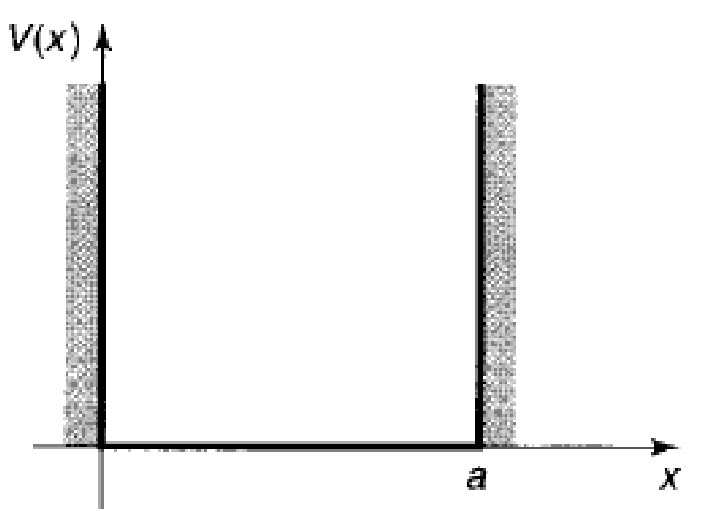
\includegraphics[width=0.5\textwidth]{figure/inftypotential.jpg}
    \caption{无限深势阱的势能示意图}
    \label{fig3:inftypotential}
\end{figure}

由于势场在除了$0\leq x\leq a$处都是无穷大的,因此粒子被束缚在了[0,a]中,我们只需要讨论这个范围中的运动情况即可。此时的Schrodinger方程为:
\begin{equation}
    E\psi =-\frac{\hbar^2}{2m}\frac{d^2\psi}{dx^2}
\end{equation}

其中E是能量本征态,我们可以将上式简写为:
\begin{equation}\label{equ3:string}
\frac{d^2\psi}{dx^2}+k^2\psi =0    
\end{equation}

其中$k=\sqrt{\frac{2mE}{\hbar^2}}$,求解微分方程得到该方程的通解:
\begin{equation}
    \psi =Acoskx+Bsinkx
\end{equation}

随后我们考虑初值问题,由于波函数一定是单值,连续,归一的,而边界上,波函数的势能无限大,因此出现粒子的概率一定为0,即波函数在边界上的取值为0:
\begin{equation}
    \psi(0)=\psi(a)=0
\end{equation}

当$x=0$,我们得到$A=0$;进一步的,当$x=a$,我们得到$Bsinka=0$。由于我们需要一个有意义的波函数,因此在这里$B\ne 0$(否则波函数恒为0)。于是我们可以得到边界条件为:$sinka=0$,即
\begin{equation}
    ka=n\pi ,n=0,\pm 1,\pm 2,\ldots
\end{equation}

根据边界条件,我们可以知道能量本征值的关系:
\begin{equation}
    E=\frac{k^2\hbar}{2m}=\frac{n^2\pi^2 \hbar^2}{2a^2m},n=0,1,2,\ldots 
\end{equation}

由于当$n<0$时,能量本征值与$n>0$时一一对应,并不产生新的结果。因此我们可以人为定义n的取值为正整数。最后我们通过归一化求出归一化因子B:
\begin{equation}
    \int_0^a |B|^2sin^2kx dx =1 \Rightarrow B=\sqrt{\frac{2}{a}}
\end{equation}

于是我们求得了最终的本征函数$\psi_n(x)$:
\begin{equation}
    \psi_n(x)=\sqrt{\frac{2}{a}}sin(\frac{n\pi}{a}x)
\end{equation}

对于这个简单模型,还可以从波动的角度理解:由式\ref{equ3:string},我们可以知道此时定态Schrodinger方程是一个弦振动方程。更进一步,考虑到边界条件,这应该是一个两端固定的弦振动方程,因此我们可以将这个方程的解看作一种驻波,此时势阱宽a满足驻波条件:
\begin{equation}
    a=\frac{\lambda}{2}\cdot n
\end{equation}

这里的$\lambda$是De Brogile 驻波对应的波长。

\begin{figure}[htp]
    \centering
    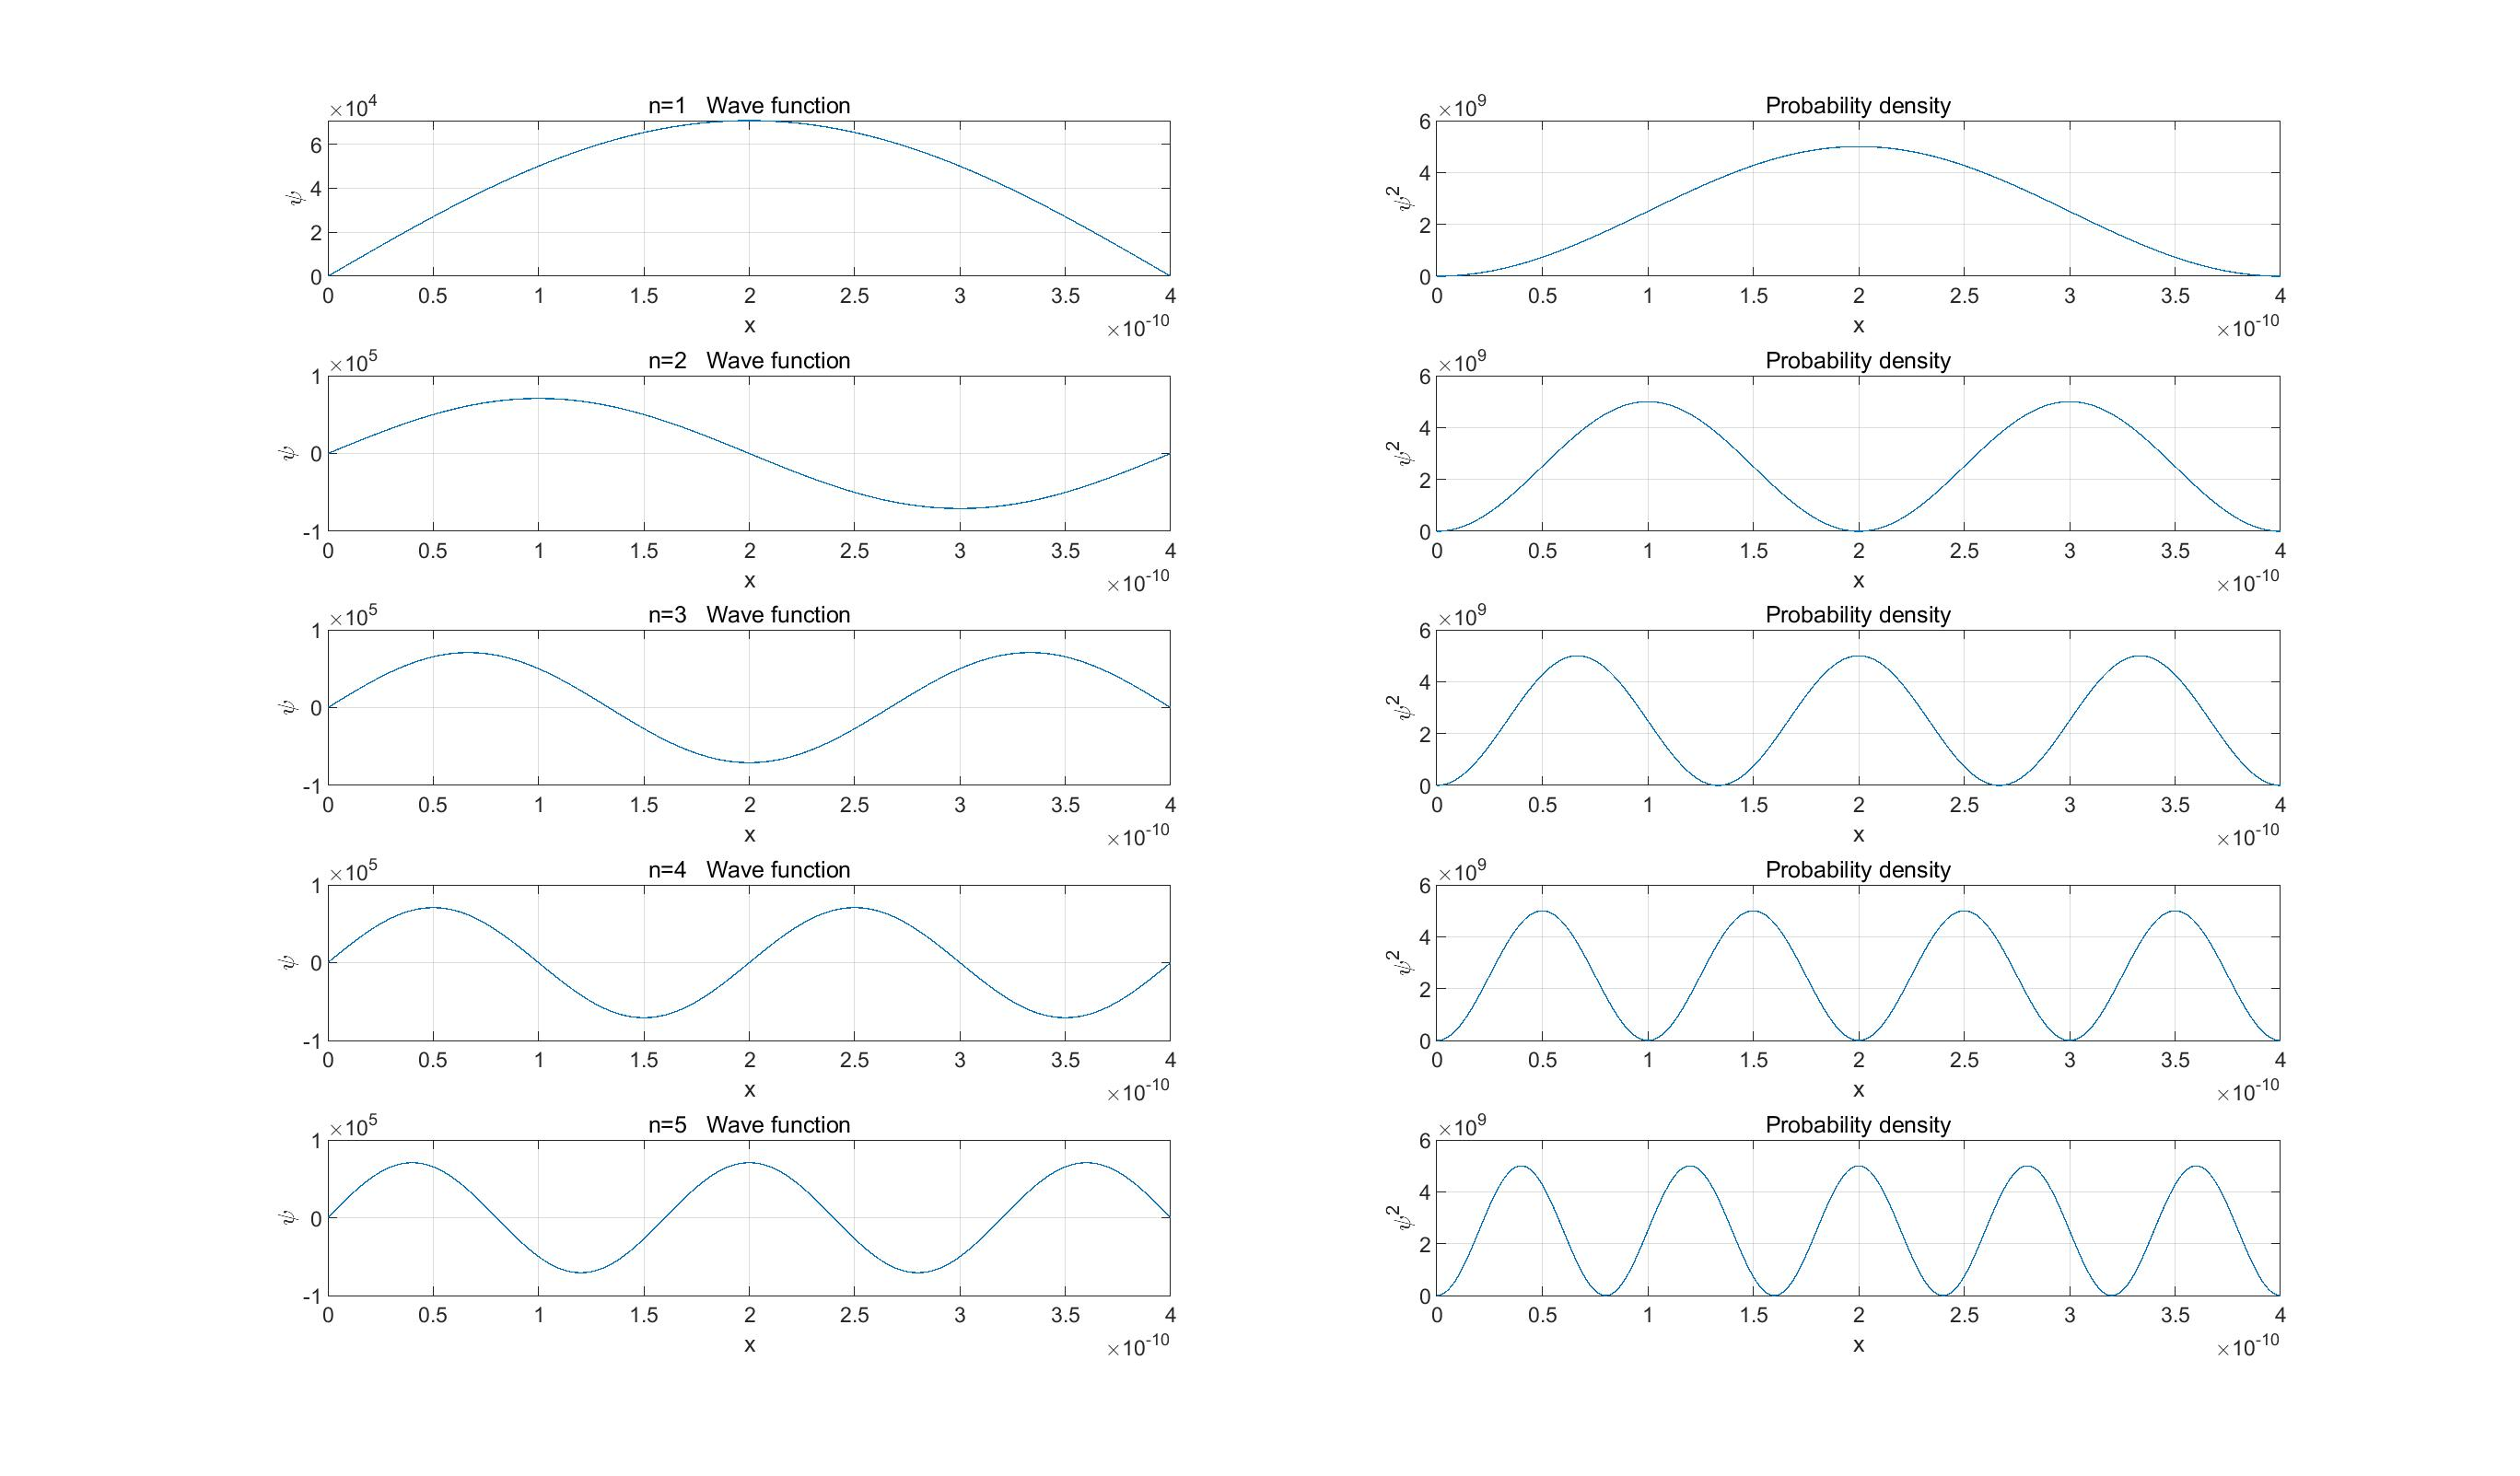
\includegraphics[width=0.9\textwidth]{figure/1Dinfinite.jpg}
    \caption{电子一维无限深势阱的波函数和概率密度示意图\footnote{其中$a=4\times 10^{-10}m$}}
    \label{infinite}
\end{figure}
\section{半无限深势阱}
本节我们讨论一个相对无限深势阱复杂的模型---半无限深势阱,其势能函数形式如下:
\begin{align}
V(x)=\left\{
    \begin{array}{ll}
       0  & 0\leq x\leq a \\
        +\infty & x<0\\
        V_0 & x>a
    \end{array}\right.
\end{align}

对于$0\leq x\leq a$的情况来说,方程形式与式\ref{equ3:string}完全一样,结合一边的边界条件,我们可以得到其通解同样为$\psi(x)=Bsinkx$,其中$k=\sqrt{\frac{2mE}{\hbar^2}}$。现在考虑$x>a$时的情况,事实上我们可以发现,方程同样可以写成式\ref{equ3:string}的形式:
\begin{equation}
    \frac{d^2\psi}{dx^2}+K^2\psi=0
\end{equation}

其中$K=\sqrt{\frac{2m(E-V)}{\hbar^2}}$。下面我们分别考虑几种可能的情况:
\begin{enumerate}
    \item $K<0$,此时$\psi(x)=CcosKx+DsinKx$,不满足波函数归一化推论:$\psi(+\infty)=0$的条件,固舍去;
    \item $K=0$,此时$\psi(x)=C+Dx$,同样不满足波函数归一化推论:$\psi(+\infty)=0$的条件,固舍去;
    \item $K>0$,此时$\psi(x)=Ce^{-Kx}+De^{Kx}$,由于波函数归一化推论:$\psi(+\infty)=0$,因此得到$D=0$,因此通解为$\psi(x)=Ce^{-Kx}$
\end{enumerate}

由于波函数应该是连续的,因此在$x=a$处的波函数与波函数的导数应该是对应相等的,即\footnote{这里波函数的导数相等是考虑到连续的定义,否则左右极限不相等,这个点无法用Schrodinger方程进行分析}:
\begin{align}
    \begin{split}\label{equ3:hinf_pre}
        Bsinka= & Ce^{-Kx}\\
        Bkcoska= & -CKe^{-Kx}
    \end{split}
\end{align}

两式相除,得到:
\begin{equation}\label{equ3:hinf}
    cotka=\frac{K}{k}
\end{equation}

这是一个超越方程,无法得到精确解,我们可以采用计算机数值求解的方法。在数学上,我们还可以通过将这个超越方程转化为两条函数曲线的交点问题,直观定性的对解进行分析。要想将问题转化为两条曲线的交点问题,需要统一等号两端的变量。令$X=ka,\beta=\sqrt{\frac{2mV_0}{\hbar^2}} a$,\footnote{我们常常称$\beta$ 为势场强度}于是式\ref{equ3:hinf}可以变为:
\begin{equation}
    cotX=-\sqrt{(\frac{\beta}{X})^2-1}
\end{equation}
%少图


通过图像,我们可以定性的得到一些结论:
\begin{enumerate}
    \item 由于$Y(\beta)=-\sqrt{(\frac{\beta}{X})^2-1}=0$,因此满足的能量本征态只有有限个;
    \item 与无限深势阱的驻波条件进行比较可以得,无限深势阱对应得$X=n\pi $,永远比半无限深势阱得$X$要大,并且两者之差越来越大。由图可知,当$n\rightarrow \infty $时,$n\pi-X_n\rightarrow \frac{\pi}{2}$。即两种模型的最大“能量”差;
    \item $X$的大小与取值与$\beta$息息相关。如果$\beta <\frac{\pi}{2}$,那么束缚态系统甚至没有符合条件的能量本征态
\end{enumerate}

通过图像,或是计算机得到$X_n$以后,就可以通过定义反解出能量本征值的值了:
\begin{equation}
    E_n=\frac{\hbar^2X^2}{2ma^2}
\end{equation}

同时根据归一化条件,我们可以得到一个含有系数$B_n,C_n$的方程:
\begin{equation}
    \int_0^a|\psi_n(x)|^2dx+\int_a^\infty|\varphi_n(x)|^2dx=1
\end{equation}

其中$\psi_n(x)=B_nsink_nx,\varphi_n(x)=C_ne^{-Kx}$。将上式与\ref{equ3:hinf_pre}中的任意一个方程联立即可得到展开系数$B_n,C_n$的值。

\section{对称与不对称的有限深势阱*}
有了半无限深势阱的求解方法,我们可以自然的迁移到两边的势能函数都是有限的情况。这个时候求解过程和半无限深势阱几乎一致,因此本节的结论请读者自行验证。
\section{直链共轭体系的$\pi$电子}
 本节我们讨论势阱问题的一个简单的例子。对于直链共轭体系的$\pi$电子来说,我们可以将其看作在$\sigma$键以及其它分子相互作用产生的势场里描述共轭体系的$\pi$电子的运动。当势场为周期函数等简单的函数时,其Schrodinger方程是可以精确求解的。我们考虑的模型时一个有$2N$个链状共轭体系的分子,其中N个碳碳单键,N个碳碳双键。此时我们令一根碳碳单键与一根碳碳双键组成的周期元素长度为l,假设其中2N个$\pi$电子在总长为$L=Nl$的无限深势阱内运动,那么可以知道,任意一个电子的能级都满足:
 \begin{equation}
     E_n=\frac{n^2h^2}{8mL^2}
 \end{equation}
 
 由于电子满足泡利不相容原理,因此同一个能级最多容纳自旋相反的两个电子,因此2N个$\pi$电子应该占据N个能级。那么当日光照射到这个有机物的时候,假如光子的频率正好满足:
 \begin{equation}
     hv_n=E_n-E_{n-1},n=2,3,\dots,N
 \end{equation}
 
 那么这个频率的光就会被吸收,我们联立电子的能级公式,可以得到:
 \begin{equation}
     v_n=\frac{h}{8mL^2}(2n-1),n=2,3,\dots,N
 \end{equation}
 
 得到了吸收的频率以后,我们可以求出吸收谱对应的波长:
 \begin{equation}
     \lambda_n=\frac{c}{v_n}=\frac{8mcl^2N^2}{h(2n-1)},n=2,3,\dots,N
 \end{equation}
 
 从上式中可以得出一些定性结论:
 \begin{enumerate}
     \item 当N固定,就会对应N-1个吸收峰,我们一般考察波长最长的那个峰,当日光照射到有机物的时候,波长小于该峰的光全部被吸收掉,如果此时剩下的光的波长落在了可见光区域,那么有机物就会呈现颜色。由该式我们可以明显看到,N越大,吸收带越宽,整个吸收谱会发生红移。
     \item 
 \end{enumerate}
\section{自由粒子的散射态问题}
    \subsection{方形势垒的隧穿效应}
    
    \subsection{势垒穿透的一种理解}
    对于势垒穿透问题,我们利用测不准原理给出一个解释:\footnote{注意,这里讲的只是一种理解而并不是严格解释}对于$E<V_0$的情况,当自由粒子进入$x=0$附近的区域,我们可以认为它的位置是比较精确的,由于测不准原理,其动量具有一定的取值范围,由于动量与能量之间存在关系:$E=\frac{p^2}{2m}$,所以能量就会具有一定的取值范围,此时就会出现能量大于势能$V_0$的情况。同理,我们考虑$E<V_0$的情况,此时根据上面的叙述,当粒子处于$x=0$附近时,由于位置可以比较精确的确定,此时能量具有一定的取值范围,就会有一些能量小于势能$V_0$被反射回去。
    \subsection{扫描隧道显微镜(STM)原理简介}
    扫描隧道显微镜是基于隧穿效应的的一种“电子显微镜”。它的具体原理是这样的(如图\ref{fig:STM}):简单说来就是利用一根探针(tip),在探针和样品的表面加上电压,如果探针和样品相距很近(大约是纳米级别的距离),由于电子的质量很小,根据,隧穿效应就会比较明显,探针上的原子就会穿过空隙(势垒)进入样品,形成极其微弱的电流。这样,我们通过记录电流的情况就能记录样品表面的精细结构。
    
    STM主要有两种工作模式:恒流模式(constant current mode)和恒高模式(constant height mode)\footnote{具体可以参考wiki的相关内容:$https://en.jinzhao.wiki/wiki/Scanning\_tunneling\_microscope$}。在恒流模式下,反馈电子调节高度通过一个电压到压电高度控制机构。如果在某一点的隧穿电流低于设定的水平(the set level),尖端就向样品移动,反之亦然。这种模式需要的时间较长,因为电子设备需要检查隧道电流,并在表面每个测量点的反馈回路中调整高度。当表面是原子级别的平面时,施加在z轴扫描器上的电压将主要反映局部电荷密度的变化。但当遇到原子台阶(atomic step),或当表面因重组而弯曲时,扫描器的高度也将因整体地形而改变。因此,当尖端扫描表面时,为了保持隧穿电流恒定,需要z轴扫描仪的电压形成的图像将包含地形和电子密度数据。在某些情况下,人们可能不清楚探针高度的变化是由其中的哪一种因素造成的。
    
    在恒定高度模式下,当扫描器在表面来回摆动时,z轴扫描器的电压保持恒定,并映射出与距离成指数关系的隧穿电流。这种操作方式更快,但在粗糙的表面上,可能存在大的吸附分子,可能会导致探针磨损。
    \begin{figure}[H]
        \centering
        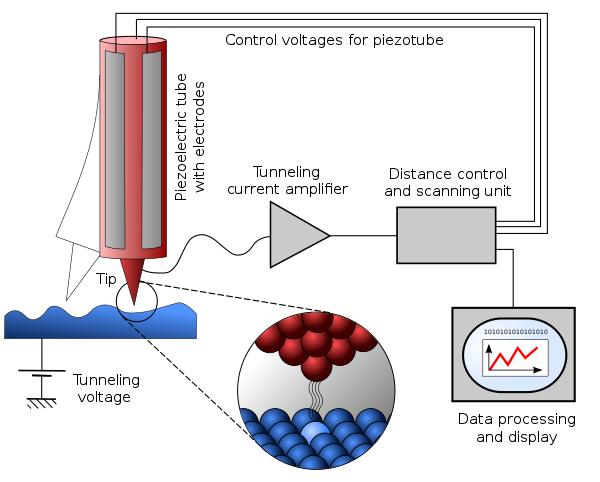
\includegraphics[width=0.9\textwidth]{figure/STM.png}
        \caption{扫描隧道显微镜的基本原理}
        \label{fig:STM}
    \end{figure}


\chapter{谐振子}
    \begin{introduction}
    \item 经典谐振子
\end{introduction}

\section{经典谐振子}
经典谐振子的运动模式遵循Hooke定律,即满足:
\begin{equation}
    F=-kx
\end{equation}

其中$F$称为回复力,$k$称为弹簧的弹性系数。我们对Hooke定律运用Newton第二定律,即可得到经典谐振子的运动方程:
\begin{equation}
    \frac{d^2x}{dt^2}+\omega^2x=0
\end{equation}

其中$\omega=\sqrt{\frac{k}{m}}$,称为弹簧的角频率,是描述弹簧本身性质的物理量。求解这个方程,我们可以得到位移随时间的变换关系,也就是方程的通解:
\begin{equation}
    x(t)=A\cos{\omega t}+B\sin{\omega t}
\end{equation}

其中系数A和B可以根据初始条件求得。进一步,我们可以求出弹簧的势能为:
\begin{equation}
    V(x)=\frac{1}{2}kx^2
\end{equation}

当然上述两式只能描述简谐振动的情况,因为不仅要忽略外力的作用,而且当弹簧拉伸接近或者超过弹性系数的时候,Hooke定律都是不适用的,但是当势能取极小值的时候,我们还是能够用简谐振动近似极小点附近运动的情况的(如\ref{fig:HookeLaw}):
\begin{figure}[H]
    \centering
    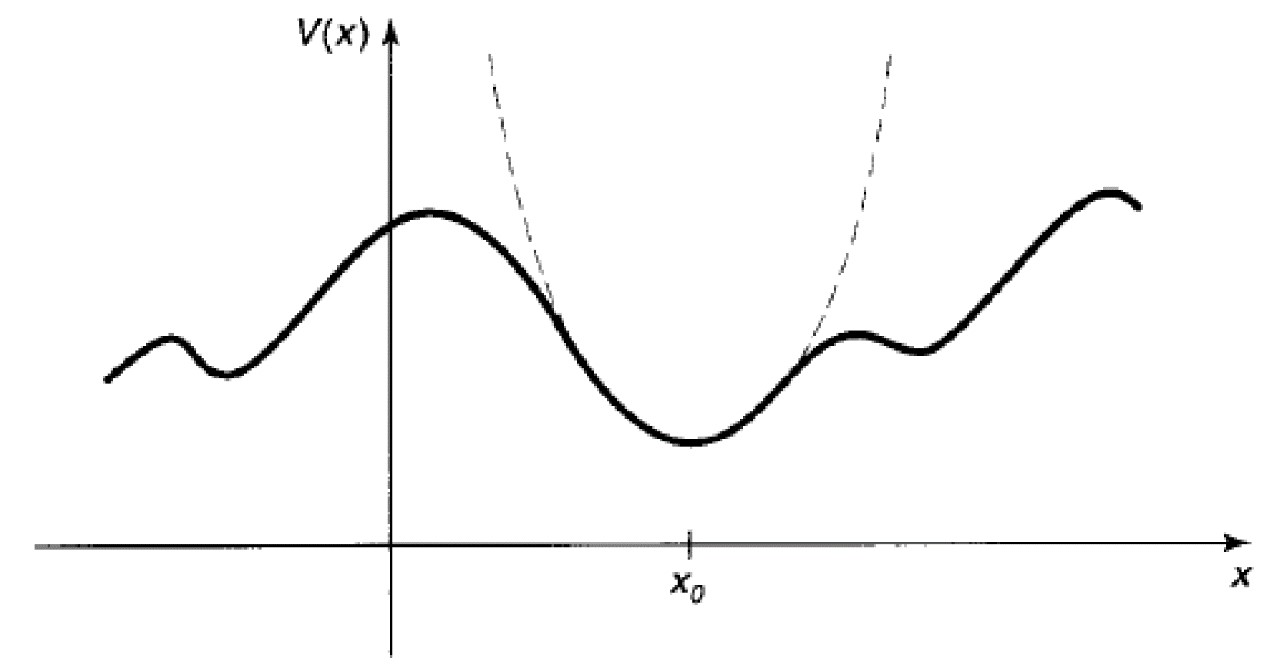
\includegraphics[width=0.9\textwidth]{figure/HookeLaw.jpg}
    \caption{简谐振动能够近似极小点附近的运动情况}
    \label{fig:HookeLaw}
\end{figure}

具体来说,我们可以对势能函数的极小点作Taylor展开:
\begin{equation}
    V(x)=V(x_0)+V'(x_0)(x-x_0)+\frac{1}{2}V''(x_0)(x-x_0)^2+\dots
\end{equation}

由于$x_0$是极小点,因此我们可以人为地令$x=x_0$处于势能零点,因此$V(x_0)=0$。同时,由于极小点的性质,$V'(x_0)=0$,所以势能函数在忽略高阶无穷小量时可以写成:
\begin{equation}
    V(x)\cong \frac{1}{2}V''(x_0)(x-x_0)
\end{equation}

这正是描述简谐运动的势能,其有效弹性系数为$k=V''(x_0)$。虽然简谐运动是简化的模型,但是其在实际情况中的实用性使得研究简谐振动是非常有必要的。


\chapter{角动量理论}
    %Chapter5 角动量理论与自旋
\begin{introduction}
    \item 角动量与旋转不变性 \ref{section5.2}
    \item 角动量的代数求解  \ref{section5.3}
    \item 电子的自旋角动量 \ref{section5:spin}
    \item 角动量的耦合 \ref{section5:coupling}
\end{introduction}
%5.1节角动量概述
\section{角动量概述}
本节我们来研究量子力学的角动量,这里涉及的领域非常重要,很多结果已经渗透到物理学的方方面面,比如:原子光谱、分子光谱;基本粒子的自旋与磁性等。在本章涉及的角动量大体分为两种,一种角动量是与经典角动量对应的。比如在经典力学中,如果一个质量为$m$的质点$P$处于有心势场\footnote{有心势场指的是势能函数只和$P$与空间中给定一点(我们设为原点$O$)的距离有关}中,则$P$点受到的力总是指向$O$,因而该点相对于$O$点的力矩为0,于是满足角动量定理:

\begin{equation}
     \frac{d}{dt}L=0
\end{equation}

而所有这些性质在量子力学中都有对应,我们在中会详细的说明。而另一方面,在20世纪发现了许多违背当时理论的实验现象,比如$Stern-Galach$实验、$Zeeman$效应等,这些现象用经典对应的角动量理论是不能解释的,因此科学家认为,一定还存在一种“典型量子化”的角动量,也就是说,这种角动量只和粒子的内禀性质有关。于是我们称第一种情况下的角动量为轨道角动量,其对应的观察算符用$\hat{L}$表示;而后一种典型量子化的角动量我们统称为自旋角动量,我们用符号$\hat{S}$表示。对于基本粒子组成的体系来说,各个轨道角动量$\hat{L_i}$之间相互组合,并且同时与各个自旋角动量相互组合构成了总角动量$\hat{J}$。本章首先讨论角动量$\hat{J}$的普遍性质,随后进一步讨论自旋的性质,最后探讨角动量的耦合作用。

\begin{remark}
\underline{\textbf{如果没有特别说明是哪种角动量,我们统一用$\hat{J}$表示任意的角动量。}}
\end{remark}
%5.2节 角动量的普遍性质
\section{角动量的普遍性质}
本节的目标是得到角动量的普遍性质。我们首先从经典力学的角动量出发,通过正则量子化得到轨道角动量$\hat{L}$的对易关系;随后通过了解角动量的本质是空间转动群的生成元,将角动量的对易关系扩展到一般的角动量$\hat{J}$上,最后利用对易关系以及谐振子中提到的代数方法得到角动量的本征值与本征函数性质。
    \subsection{轨道角动量的性质}
    在经典力学中,我们知道角动量的定义为:
    \begin{equation}\label{equ:5.2}
    L=r\times p
    \end{equation}

    在高等数学中,我们已经知道了叉乘的计算方法,于是我们可以将式\ref{equ:5.2}展开成分量形式:
    \begin{equation}
        L=(L_x,L_y,L_z)=
        \begin{vmatrix}
        e_x & e_y & e_z\\
        x & y & z\\
        p_x & p_y & p_z
        \end{vmatrix}
         =(yp_z-zp_y,zp_x-xp_z,xp_y-yp_z)
    \end{equation}

    观察轨道角动量$x$轴分量$L_x=yp_z-zp_y$,由于它$Hermite$的,因此我们可以将其进行正则量子化:
    %多行公式标记为一行用equation+split
    \begin{equation}
        \begin{split}
            \hat{L_x}&=\hat{y}\hat{p_z}-\hat{z}\hat{p_y}\\
            \hat{L_y}&=\hat{z}\hat{p_x}-\hat{x}\hat{p_z}\\
            \hat{L_z}&=\hat{x}\hat{p_y}-\hat{y}\hat{p_x}
     \end{split}
    \end{equation}
   
    于是我们可以得到轨道角动量分量之间的对易子关系:
    \begin{align}
        \begin{split}
            [ \hat{L_x},\hat{L_y} ] =&[\hat{y}\hat{p_z}-\hat{z}\hat{p_y},\hat{z}\hat{p_x}-\hat{x}\hat{p_z}] \\
            =&\hat{y}[\hat{p_z}\hat{z}]\hat{p_x}+\hat{x}[\hat{z},\hat{p_z}]\hat{p_y}\\
            =& i\hbar(\hat{x}\hat{p_y}-\hat{y}\hat{p_x})\\
            =& i\hbar \hat{L_z}
        \end{split} 
    \end{align}
       
    同理,其他分量也有关系:
    \begin{align}
        \begin{split}
            [ \hat{L_y},\hat{L_z} ] =& i\hbar \hat{L_x}\\
            [ \hat{L_z},\hat{L_x} ] =& i\hbar \hat{L_y}
        \end{split}
    \end{align}
       
     此外,对于角动量,还有一个非常重要的算符,即角动量平方算符$\hat{L^2}$,我们可以验证$\hat{L^2}$和角动量分量对易:
       \begin{align}
        \begin{split}
            [ \hat{L^2},\hat{L_x} ] =& [\hat{L^2_x}+ \hat{L^2_y} + \hat{L^2_z},\hat{L_x}]\\
          =&[\hat{L^2_y} + \hat{L^2_z},\hat{L_x}]\\
          =& \hat{L_y} [\hat{L_y},\hat{L_x}] + [\hat{L_y},\hat{L_x} ]\hat{L_y}
          + \hat{L_z} [\hat{L_z},\hat{L_x}] + [\hat{L_z},\hat{L_x}] \hat{L_z}\\
          =&i\hbar(-\hat{L_y}\hat{L_z}-\hat{L_z}\hat{L_y}+\hat{L_z}\hat{L_y}+\hat{L_y}
          \hat{L_z})\\
          =&0
        \end{split}
    \end{align}
    
     这个性质说明我们至少可以选取角动量平方算符$\hat{L^2}$和其中一个方向的角动量算符
     \footnote{在这里我们需要注意,由于之前我们已经证明了角动量算符分量之间不对易,因此我们只能同时取一个分量算符}
     $\hat{L_i}$(我们常常选用$z$方向上的角动量算符\footnote{原因可能在于在取诸如柱坐标、球坐标的情况下,$z$方向下的算符形式是最简单的})作为ESCO的一部分。这个性质是后续关于角动量、氢原子内容的基础。
     
 %角动量与旋转这一节需要参考群论教材
    \subsection{角动量与旋转} \label{section5.2}
 
    \subsection{角动量的代数求解方法}\label{section5.3}
        \subsubsection{角动量的本征值问题}\label{section5.3.1}
        在上一节中,我们已经知道了一般角动量$\hat{J}$由于保持了旋转群的局域结构,因此对易子的形式与轨道角动量类似:
         \begin{align}
             \begin{split}
                [ \hat{J_x},\hat{J_y} ] =& i\hbar \hat{J_z}\\
                 [ \hat{J_y},\hat{J_z} ] =& i\hbar \hat{L_x}\\
                [ \hat{J_z},\hat{J_x} ] =& i\hbar \hat{J_y}\\
                [ \hat{J^2},\hat{J_z} ] =&0
            \end{split}
        \end{align}   
        因此我们考虑$\hat{J^2},\hat{J_z}$的共同本征态和本征值的形式,即对于本征态$|\psi \rangle$,考虑本征方程:
        \begin{align}\label{equ:5.9}
            \begin{split}
                \hat{J^2}|\psi \rangle = \lambda |\psi \rangle\\
                \hat{J_z}|\psi \rangle=\mu |\psi \rangle
            \end{split}
            \end{align}   
            
        本节我们的目的是求得$\lambda,\mu$之间的关系。这里我们采用与谐振子一样的思路,通过算符的“对称化”的思路构造如下升降算符$\hat{J_\pm}$:
         \begin{align}
            \begin{split}
                \hat{J_+}=\hat{J_x}+i\hat{J_y}\\
                \hat{J_-}=\hat{J_x}-i\hat{J_y}
            \end{split}
        \end{align} 
            
        根据定义,上升算符与下降算符虽然不是Hermite算符,但是可以验证,它们互为伴随算符:
        \begin{equation}
           ( \hat{J_+})^\dagger = \hat{J_-}
        \end{equation}
        
        我们可以想象,升降算符作用的好处在于我们可以获得多次作用后的本征方程,但是根据式\ref{equ:5.9}的形式,我们需要利用升降算符与$\hat{J^2}$和$\hat{J_z} $的对易子进行转化,首先考虑对易关系:
         \begin{align}\label{equ:5.12}
            \begin{split}
                [\hat{J_\pm},\hat{J_z}]=&[\hat{J_x}\pm i\hat{J_y},\hat{J_z}]\\
                =&[\hat{J_x},\hat{J_z}]\pm i[\hat{J_y},\hat{J_z}]\\
                =&-i\hbar \hat{J_y}+i\cdot i\hbar \hat{J_x}\\
                =&\hbar (\hat{J_x}\pm i\hat{J_y})\\
                =&\hbar\hat{J_\pm }
            \end{split}
        \end{align} 
        \begin{align}\label{equ:5.13}
               [\hat{J_\pm},\hat{J^2}] =&[\hat{J_x}\pm i\hat{J_y},\hat{J^2}]=0
        \end{align}
        
        由式\ref{equ:5.12},式\ref{equ:5.13},我们可以知道$\hat{J_\pm}$对本征态$|\psi\rangle$的作用:
        \begin{align}\label{equ:5.14}
            \begin{split}
                \hat{J^2}(\hat{J_\pm}|\psi \rangle)=&-[\hat{J_\pm},\hat{J^2}]|\psi \rangle +\hat{J^2} (\hat{J_\pm}|\psi \rangle)\\
                =& \hat{J_\pm}(\hat{J^2}|\psi \rangle)\\
                =& \hat{J_\pm}\lambda|\psi \rangle
            \end{split}
        \end{align}
         \begin{align}\protect\label{equ:5.15}
            \begin{split}
                \hat{J_z}(\hat{J_\pm}|\psi \rangle)=&-[\hat{J_\pm},\hat{J_z}]|\psi \rangle +\hat{J_z} (\hat{J_\pm}|\psi \rangle)\\
                =& \hat{J_\pm}\Big((\hat{J_z}+\hbar) |\psi \rangle \Big)\\
                =& \hat{J_\pm} \Big((\mu+\hbar) |\psi \rangle \Big)
            \end{split}
        \end{align}
        
        对于式\ref{equ:5.14},\ref{equ:5.15},我们可以很容易地推广到n个升降算符对态矢量$|\psi \rangle$的共同作用:
        \begin{align}
                \hat{J_z}\Big( (\hat{J_\pm} )^n|\psi \rangle \Big)
                =& (\mu \pm n\hbar) \Big((\hat{J_\pm})^n|\psi \rangle \Big)\\
                \hat{J^2}\Big((\hat{J_\pm})^n|\psi \rangle \Big) 
                =&\lambda\Big((\hat{J_\pm})^n|\psi \rangle \Big) \label{equ:5.17}
        \end{align}
        
        对于一个物质的总角动量,可以想象它的取值一定不会无限大或无限小,一定存在上下限。首先我们考虑$\hat{J_z}$的上限,假设经过$N$次上升算符作用后$\hat{J_z}$的本征值达到了最大值$l\hbar$:
        \begin{align}\label{equ:5.18}
             \mu + N\hbar = j\hbar \\
             \hat{J_z}|\psi _j\rangle= j\hbar |\psi _j\rangle \label{equ:5.18.2}
        \end{align}
        
        如果我们记$(\hat{J_+})^N|\psi \rangle=|\psi _j\rangle$,那么一定有本征方程:
        \begin{align} \label{equ:5.19}
             \hat{J_+}|\psi _j\rangle= 0\\
             \hat{J^2}|\psi _j\rangle= \lambda|\psi _j\rangle \label{equ:5.20}
        \end{align} 
        
        现在我们已经通过上限关系式\ref{equ:5.18}的确定将$\lambda,\mu$的关系转变为了求得上限$l$与$\lambda$的关系,但不同的地方在于,相比于一开始的“茫然无措”,这次我们多了几个“好帮手”---即式\ref{equ:5.19},\ref{equ:5.20}和\ref{equ:5.18.2}三式。这里继续求解的思路是将$\hat{J^2}$展开为$\hat{J_+},\hat{J_z}$的形式,结合$\hat{J^2}$算符的本征方程(式\ref{equ:5.17}),两式联立即可得到最后的答案,具体计算过程如下:
        
        由于$\hat{J^2}=\hat{J_x^2}+\hat{J_y^2}+\hat{J_z^2}$,因此我们首先可以通过升降算符替换掉$\hat{J_x^2}+\hat{J_y^2}$部分,通过升降算符的定义,我们可以得到:
        \begin{align}
            \begin{split}\label{equ:5.22}
                \hat{J_+}\hat{J_-}=& (\hat{J_x }+ i \hat{J_y})(\hat{J_x}- i\hat{J_y})\\
                =&\hat{J_x^2}+\hat{J_y^2}-i(\hat{J_x}\hat{J_y}-\hat{J_y}\hat{J_x})\\
                =&\hat{J_x^2}+\hat{J_y^2}+\hbar \hat{J_z}
            \end{split}
        \end{align}
        
        同理:
        \begin{align}
             \hat{J_+}\hat{J_-}=& \hat{J_x^2}+\hat{J_y^2}- \hbar \hat{J_z}
        \end{align}
        
        于是代入式\ref{equ:5.18.2},我们可以得到:
        \begin{align}\label{equ:5.24}
            \begin{split}
               \hat{J^2}|\psi_j \rangle=&(\hat{J_-}\hat{J_+} + \hbar \hat{J_z}+\hat{J_z^2})|\psi_j \rangle\\
               =&\hat{J_-}\hat{J_+}|\psi_j \rangle +\hbar \hat{J_z}|\psi_j \rangle+\hat{J_z^2}|\psi_j \rangle\\
               =& 0 +j\hbar^2 |\psi_j\rangle + j^2 |\psi_j \rangle\\
               =& j(j+1)\hbar^2 |\psi_j \rangle
            \end{split}
        \end{align}
        
        综合对比式\ref{equ:5.12},我们可以得到:
        \begin{equation}\label{equ:5.25}
            \mu = j(j+1)\hbar^2
        \end{equation}
        
        讨论完上界以后,我们采用相同的方法研究$\hat{J_z}$的下界,我们假设经过N'次下降算符作用后$\hat{J_z}$的本征值达到了最小值$j'\hbar $:
        \begin{align}\label{equ:5.26}
             \mu - N'\hbar = j'\hbar \\
             \hat{J_z}|\psi _{j'}\rangle= j'\hbar |\psi _{j'}\rangle \label{equ:5.27}
        \end{align}
        
        如果我们记$(\hat{J_-})^N|\psi \rangle=|\psi _{l'}\rangle$,那么一定有本征方程:
        \begin{align} \label{equ:5.28}
             \hat{J_-}|\psi _{j'}\rangle= 0\\
             \hat{J^2}|\psi _{j'}\rangle= \lambda|\psi _{j'}\rangle \label{equ:5.29}
        \end{align}
        
        对比式\ref{equ:5.24},我们可以类似得到:
        \begin{align}\label{equ:5.30}
            \begin{split}
               \hat{J^2}|\psi_{j'} \rangle=&(\hat{J_+}\hat{J_-}-\hbar \hat{J_z}+\hat{J_z^2})|\psi_{j’} \rangle\\
               =&\hat{J_+}\hat{J_-}|\psi_{j'} \rangle-\hbar \hat{J_z}|\psi_{j'} \rangle+\hat{J_z^2}|\psi_{j'} \rangle\\
               =& 0 -j'\hbar^2 |\psi_{j'} \rangle + {j'}^2 |\psi_{j'} \rangle\\
               =& j'(j'-1)\hbar^2 |\psi_{j'} \rangle
            \end{split}
        \end{align}
        
        于是:\label{equ:5.31}
        \begin{equation}
            \mu = j'(j'-1)\hbar^2
        \end{equation}
        
        %\textrm{}用于在公式中插入文字
        联立式\ref{equ:5.25},我们可以得到:
        \begin{equation}
            j(j+1)=j'(j-1) \longrightarrow j=j'-1 
            \quad \textrm{or} \quad j=-j'
        \end{equation}
        
        由于$j>j'$,因此第一种可能性被排除,只可能有$j'=-l$。因此$\hat{J_z}$本征值有$2j+1$种可能,而从本征值$\mu$出发,本征值可以有$N+N'+1$种取值,因此,$2j=N+N'$,该式说明$j$的可能取值为半整数。
        
        同时,根据上面的推导过程,我们可以将$\mu$写成$\hbar$的整数倍这种更为整洁的形式。综上所述,我们可以得到总角动量算符有关的本征方程:
        
        \begin{align}\label{equ:5.33}
            \hat{J^2}|\psi \rangle =&j(j+1)\hbar ^2|\psi \rangle ,j=\frac{n}{2},n\in \mathbb{Z}\\
            \hat{J_z}|\psi \rangle=&m \hbar |\psi \rangle ,m=-j,-j+1,\ldots,j-1,j
            \label{equ:5.34}
        \end{align}
        
        \subsubsection{标准表象$|k,j,m \rangle $}\label{subsubsection5:standardbasis}
        根据式\ref{equ:5.33},\ref{equ:5.34},我们已经获得了本征值之间的关系,本节我们选择一种较为通用的方法,即采用升降算符$\hat{J_+},\hat{J_-}$构造态空间上的一组完备正交基。
        
        在讨论之前,我们再复习一下一些重要的知识点。在之前的内容中,我们已经知道了$\hat{J^2},\hat{J_z}$的共同本征态并不构成态空间上的ESCO,因此我们不能用$|j,m\rangle$去描述态空间中的态,而应该额外增加一个物理量\footnote{也可以是若干个物理量,这里统一用$k$表示},加入我们用$k$代表其本征值,则态空间上任意一个态都可以用$|k,j,m\rangle$表示;同时,如果假设将$j,m$相等的态的集合记作$\mathcal{E}(j,m)$,可以简单验证,这个集合是态空间的一个子空间,其维数$dim\mathcal{E}\geq1$并且其中任意的态都是正交归一的,即:
        \begin{equation}
            \langle k_i,j,m|k_j,j,m\rangle=\delta_{ij}
        \end{equation}
        
        因此,我们的问题就转变为了:证明不同子空间的态相互正交。利用升降算符,我们可以得到态$|j,m\rangle \rightarrow |j,m\pm 1\rangle$的关系。首先,根据式\ref{equ:5.17},我们知道:
        \begin{equation}
            \hat{J_\pm }|j,m\rangle \propto |j,m\pm 1\rangle
        \end{equation}
        
        随后考虑比例系数。根据式\ref{equ:5.22},以及上升算符和下降算符的对偶性,考虑$\hat{J_+}|k_i,j,m\rangle$的标量积:
        \begin{align}
            \begin{split}
                \langle k_i,j,m|\hat{J_-}\hat{J_+}|k_s,j,m\rangle=&\langle k_i,j,m|\hat{J^2}-\hat{J_z^2}-\hbar\hat{J_z}|k_s,j,m\rangle\\
                =&\Big( j(j+1)-m(m+1)\Big)\hbar^2\langle k_i j,m|k_s,j,m\rangle
            \end{split}
        \end{align}
        
        同理:
        \begin{equation}
            \langle k_i,j,m|\hat{J_+}\hat{J_-}|k_s,j,m\rangle=\Big( j(j+1)-m(m-1)\Big)\hbar^2\langle k_i,j,m|k_s,j,m\rangle
        \end{equation}
        
        于是:\label{equ3:totangularmom}
        \begin{equation}\label{equ5:stadbasis}
            \hat{J_\pm } |k_i,j,m\rangle = \sqrt{j(j+1)-m(m\pm 1)}\hbar |k_s,j,m \pm1\rangle  \delta_{si}
        \end{equation}
        
        根据式\ref{equ5:stadbasis},我们能够通过升降算符从任意一个子空间于$\mathcal{E}(j,m)$的一组正交归一基生成任意一个子空间的一组正交归一基,具体思路如下图:
        \begin{figure}[htp]
            \centering
            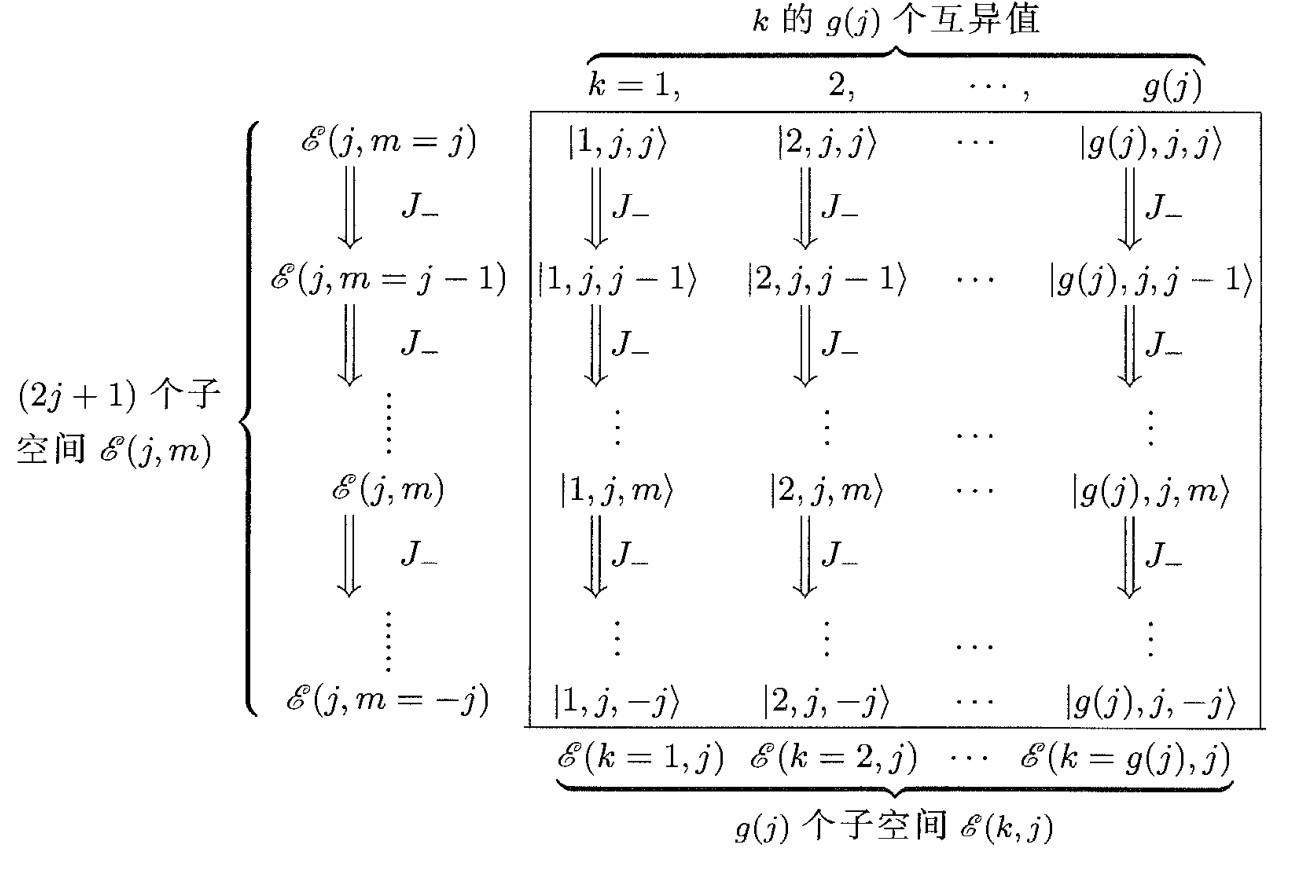
\includegraphics[width=0.9\textwidth]{figure/stadbasis.jpg}
            \caption{标准表象$|k,j,m\rangle$的生成}
            \label{fig5:standbasis}
        \end{figure}
        
        有两点值得注意的地方。首先,我们希望能用算符$\hat{A}$,使得$\hat{A},\hat{J^2},\hat{J_z}$构成态空间上的ESCO。同时,我们更希望升降算符作用以后的态仍然能够用算符$\hat{A}$来辨认,于是在这里我们需要一个额外的条件,即:$[\hat{J},\hat{A}]=0$\footnote{即算符$\hat{A}$是一个标量算符。这个想法是自然的}。
        
        其次,本节的讨论是基于$\mathcal{E}(j,m)$来构造整个态空间的正交归一基,但是在实际操作中有几个缺陷:
        \begin{enumerate}
            \item $\mathcal{E}(j,m)$的维数并不是事先知道的,与体系的性质有关系;
            \item 由于$\langle k_i,j,m|\hat{J_-}\hat{J_+}|k_s,j,m\rangle$一般不等于0,因此我们可以推出$\hat{J}|k,j,m\rangle \notin \mathcal{E}(j,m)$,即空间$\mathcal{E}(j,m)$在$\hat{J}$的作用下并不是不变的,这一点性质尤其不好。
        \end{enumerate}
        
        上述在实际操作中带来不便的因素促使我们思考另一种子空间的构造方法,即$\mathcal{E}(k,j)$。根据图\ref{fig5:standbasis}可知$\mathcal{E}(k,j)$的组成,经过简单演算我们可以知道以下两点:
        \begin{enumerate}
            \item $\mathcal{E}(k,j)$的简并度永远不变,等于$2j+1$
            \item $\mathcal{E}(k,j)$在$\hat{J},\hat{J^2},F(\hat{J})$下都保持不变
        \end{enumerate}
        
        本节我们只是简单的对总体情况做一个说明,在后面的内容中(尤其是对角动量的耦合以及氢原子的讨论),我们会有更多的实例来佐证本节的观点。
\section{自旋}\label{section5:spin}
    \subsection{自旋的实验引入}
    
    
    \subsection{$\frac{1}{2}$自旋态的表示}
        在上节的最后,我们提到了自旋角动量只与粒子本身的内禀属性有关。事实上,自旋角动量是一个相对论效应,Dirac通过建立Dirac方程可以来描述电子的自旋。由于本笔记在不说明的情况下都是仅仅讨论非相对论的量子力学,因此在本节中,我们采用Pauli的理论,通过加入一些假设使得自旋自洽的融入其中。
        
        由于电子的自旋是一个新的自由度,并且对于电子,我们可以通过量子电动力学证明$s=\frac{1}{2}$,则$m_s=\frac{\hbar}{2},-\frac{\hbar}{2}$。于是我们认为电子状态波函数是一个二分量的列旋量\footnote{这里注意,电子状态波函数构成的不是二分量的列矢量,因为自旋空间上的运动会影响位形空间 上的运动}。
        \begin{equation}
            |\psi(r,s_z,t)\rangle=\binom{\psi_1(r,t)}{\psi_2(r,t)}=\psi_1(r,t)|\alpha \rangle+\psi_2(r,t)|\beta\rangle
        \end{equation}
        
        其中我们认为$|\alpha\rangle$是自旋向上的,$|\beta\rangle$是自旋向下的,并且定义$|\alpha\rangle=\binom{1}{0},|\beta\rangle=\binom{0}{1}$。如果体系的$Hamiltonian$不含自旋角动量,或者自旋部分和空间部分可以分开\footnote{即$\hat{H}=\hat{H_s}+\hat{H_r}$},那么自旋态与位形空间上的态就可以分离:
        \begin{align}
            \begin{split}
                |\psi(r,s_z,t)\rangle=|\varphi(r,t)\rangle|\xi(s_z,t)\rangle\\
                |\xi(s_z,t)\rangle=\binom{\xi_1(t)}{\xi_2(t)}=\xi_1(t)|\alpha\rangle+\xi_2(t)|\beta \rangle
            \end{split}
        \end{align}
        
        于是在考虑自旋角动量后,我们可以将Schrodinger方程改写为两分量的方程,我们称之为Pauli方程。
        
        
        在\ref{section5.3.1}中,我们已经得到了角动量的一般理论,现在我们将其应用于自旋中,可以得到自旋角动量算符的对易关系和本征方程:
        \begin{align}
            \begin{split}
             [\hat{S_x},\hat{S_y}]=&i\hbar\hat{S_z}\\
             [\hat{S_x},\hat{S_y}]=&i\hbar\hat{S_z}\\
             [\hat{S_x},\hat{S_y}]=&i\hbar\hat{S_z}\\
            [\hat{S^2},\hat{S_i}]=0,i=&x,y,z\\
            \hat{S^2}|\psi\rangle=s(s+1)\hbar&|\psi\rangle\\
            \hat{S_z}|\psi\rangle=m_s\hbar|\psi\rangle,m_s=&s,s-1,\ldots,-s+1,-s
            \end{split}
        \end{align}
        
       由于自旋波函数是一个两分量的列旋量,因此自旋角动量分量算符$\hat{S_i}$一定可以表示成$2\times 2$的Hermite矩阵\footnote{下文讲述的只是自旋矩阵的一种常用表象,即Pauli表象而已,事实上我们并不能完全确定矩阵的具体性质,但是我们可以证明这三个矩阵一定是自逆,反对易,零迹的,详见张永德《量子力学》(第四版),科学出版社,p176-p179}。同时,由于态空间可以表示为自旋空间和位形空间的直积($\mathcal{E}=\mathcal{E}_r\otimes\mathcal{E}_s$),因此与自旋角动量有关的算符(如$\hat{S_z}$)可以作为$\mathcal{E}_s$空间上的延申算符。如果我们进一步假设$\hat{S_z}$的本征态是非简并的,于是我们有以下关系:
        \begin{align}
            \begin{split}
                \hat{S_z}|\alpha\rangle=&\frac{1}{2}\hbar|\alpha \rangle\\
                \hat{S_z}|\beta \rangle=&-\frac{1}{2}\hbar|\beta \rangle
            \end{split}
        \end{align}
        
        其中,由于$|\alpha \rangle,|\beta \rangle$是正交归一的,因此我们可以将$\{|\alpha \rangle,|\beta \rangle \}$看作自旋空间$\mathcal{E}_s$的基\footnote{这句话是显然的,但是由于概念比较重要,故在此多重复几遍},于是$\hat{S_z}$的矩阵形式为:
        \begin{equation}
        \hat{S_z}=\frac{\hbar}{2}
            \begin{pmatrix}
            1 & 0\\
            0 & -1
            \end{pmatrix}
        \end{equation}
    
        下面继续讨论其他两个自旋角动量分量算符对应的矩阵形式。根据\ref{equ3:totangularmom},我们知道,对于自旋空间上的态,升降算符的作用可以表示为:
        \begin{equation}
            \hat{J_\pm}|s,m_s\rangle=\sqrt{s(s+1)-m_s(m_s\pm 1)}\hbar |s,m_s-1\rangle
        \end{equation}
        
        将$s=\frac{1}{2},m_s=\frac{1}{2},-\frac{1}{2}$代入,可得\footnote{在这里$|\alpha\rangle=|\frac{1}{2},\frac{1}{2}\rangle,|\beta\rangle=|\frac{1}{2},-\frac{1}{2}\rangle$}:
        \begin{align}
            \begin{split}
                \hat{S_+}|\alpha\rangle=\hat{S_-}|\beta\rangle=0\\
                \hat{S_+}|\beta\rangle=\hbar |\alpha\rangle\\
                \hat{S_-}|\alpha\rangle=\hbar |\beta \rangle
            \end{split}
        \end{align}
        
        于是我们得到升降算符的矩阵形式:
        \begin{equation}
        \hat{S_+}=\hbar 
            \begin{pmatrix}
            1 & 0\\
            0 & 0
            \end{pmatrix}
        \end{equation}
        
        \begin{equation}
         \hat{S_-}=\hbar 
            \begin{pmatrix}
            0 & 0\\
            0 & 1
            \end{pmatrix}
        \end{equation}
        
        联立升降算符定义:$\hat{J_\pm}=\hat{J_+}\pm \hat{J_-}$和角动量算符分量算符的对易关系:$[\hat{S_x},\hat{S_y}]=i\hbar\hat{S_z}$,并且利用角动量分量算符是Hermite的,我们可以得到角动量分量算符的矩阵形式\footnote{再次重复,这里得到的矩阵形式只是$\{\hat{S_i}\}$的一种表象,被称为Pauli表象,实际上矩阵的形式是不确定的。在这里Pauli表象有两个约定:1、$\hat{S_z}$是对角的(或者等价说法是本征态是非简并的);2、$\hat{S_x}$的相位为0。显然,不同的表象之间利用某个$2\times2$的幺正变换矩阵相互联系}:
          \begin{equation}
        \hat{S_z}=\frac{\hbar}{2}
            \begin{pmatrix}
            1 & 0\\
            0 & -1
            \end{pmatrix}
        \end{equation}
          \begin{equation}
        \hat{S_x}=\frac{\hbar}{2}
            \begin{pmatrix}
            0 & 1\\
            -1 & 0
            \end{pmatrix}
        \end{equation}
          \begin{equation}
        \hat{S_y}=\frac{\hbar}{2}
            \begin{pmatrix}
            0 & -i\\
            i & 0
            \end{pmatrix}
        \end{equation}
       
       我们可以简记为$\hat{S_i}=\frac{\hbar}{2}\hat{\sigma_i}$,其中$\hat{\sigma_i}$被称作Pauli矩阵。由于$\hat{\sigma_x},\hat{\sigma_y},\hat{\sigma_z}\textrm{和单位矩阵}\hat{\sigma_0}$在$2\times2$复矩阵空间中是线性无关的,并且该空间的维数为4,因此$\hat{\sigma_x},\hat{\sigma_y},\hat{\sigma_z},\hat{\sigma_0}$一定构成$2\times2$复矩阵空间的一组基;也就是说,任意一个$2\times2$复矩阵都能表示成$\hat{\sigma_x},\hat{\sigma_y},\hat{\sigma_z},\hat{\sigma_0}$的线性组合\footnote{注意这里的展开系数是复数}。由于Pauli矩阵具有自逆,反对易性,零迹,为展开后的计算提供了便利。
\section{角动量的耦合}\label{section5:coupling}
    \subsection{为什么要讨论角动量的耦合?}\label{subsection5:coupling}
    本节我们简单讨论一下角动量的耦合给我们计算和处理问题带来了哪些便利,首先还是考虑经典力学模型。对于N个粒子的体系,给定原点O的总角动量可以表示成各粒子角动量之和:
    \begin{equation}
        L=\sum_{i=1}^{N}L_i
    \end{equation}
    
    其中$L_i=r_i\times p_i$。在经典力学中,一个重要的思考方式就是讨论各个物理量对时间的导数。如果导数为0,则称这个物理量为运动产量(或守恒量)。由于总角动量对时间的导数等于各个粒子对O点的力矩之和:
    \begin{equation}
        \frac{dL}{dt}=\sum_{i=1}^{N}M_i
    \end{equation}
    
    如果每个粒子不受外力(即$F_{i,external}=0$),或者每个粒子的力指向同一中心,则$dL/dt=0$,总角动量是运动常量。重要的点在于,总角动量是运动常量并不能代表每个粒子的角动量也是运动常量,如果每个粒子间存在相互作用,那么粒子间的内力会引起角动量的“传递”。
    
    现在考虑量子体系。假设有两个无相互作用、无自旋的粒子,它们的总$Hamiltonian$可以表示为$\hat{H}=\hat{H_1}+\hat{H_2}$,其中:
    \begin{align}
        \begin{split}
            \hat{H_1}=-\frac{\hbar^2}{2\mu_1}\nabla^2+\hat{V}(r_1)\\
            \hat{H_2}=-\frac{\hbar^2}{2\mu_2}\nabla^2+\hat{V}(r_2)
        \end{split}
    \end{align}
    
    我们可以从中计算出:
    \begin{equation}
        [\hat{L_1},\hat{H}]=[\hat{L_2},\hat{H}]=0
    \end{equation}
    
    因此如果粒子之间没有相互作用,那么它们的角动量算符都是运动常量。但是如果两个粒子之间存在相互作用\footnote{此处假设相互作用是保守力,即对应的势能只和$|r_1-r_2|$有关},此时总$Hamiltonian$可以表示为:$\hat{H}=\hat{H_1}+\hat{H_2}+\hat{V}(|r_1-r_2|)$。此时粒子的角动量就不是运动常量了,因为:
    \begin{equation}
        [\hat{L_1},\hat{H}]=[\hat{L_1},\hat{V}(|r_1-r_2|)]
    \end{equation}
    
    上式一般不等于0,比如我们可以取$L_1$的一个分量进行计算:
    \begin{align}
            [\hat{L_{1z},\hat{H}}]=[\hat{L_{1z}},\hat{V}(|r_1-r_2|)]
            =\frac{\hbar}{i}[\hat{x_1}\frac{\partial \hat{V}}{\partial \hat{y_1}}-\hat{y_1}\frac{\partial \hat{V}}{\partial \hat{x_1}}]
    \end{align}
    
    上式一般不等于0。但是如果考虑总角动量$\hat{L}=\hat{L_1}+\hat{L_2}$,那么可以验证总角动量就是运动常量:
    \begin{align}
        \begin{split}
            [\hat{L_z},\hat{H}]=&[\hat{L_{1z}}+\hat{L_{2z}}]\\
            =&\frac{\hbar}{i}[\hat{x_1}\frac{\partial \hat{V}}{\partial \hat{y_1}}-\hat{y_1}\frac{\partial \hat{V}}{\partial \hat{x_1}}+\hat{x_2}\frac{\partial \hat{V}}{\partial \hat{y_2}}-\hat{y_2}\frac{\partial \hat{V}}{\partial \hat{x_2}}]\\
            =&\frac{\hbar}{i}\frac{\hat{V'}}{|r_1-r_2|}[\hat{x_1}(\hat{y_1}-\hat{y_2})-\hat{y_1}(\hat{x_1}-\hat{x_2})+\hat{x_2}(\hat{y_2}-\hat{y_1})-\hat{y_2}(\hat{x_2}-\hat{x_1})]\\
            =&0
        \end{split}
    \end{align}
    
    其中:
    \begin{align}
        \begin{split}
            \frac{\partial \hat{V}}{\partial \hat{y_1}}=&\frac{\partial V}{\partial|r_1-r_2|}\frac{\partial|r_1-r_2|}{\partial y_1}\\
            =&V'\frac{\partial \Big((x_1-x_2)^2+(y_1-y_2)^2+(z_1-z_2)^2\Big)^{\frac{1}{2}} }{y_1}\\
            =&\frac{V'(y_1-y_2)}{|r_1-r_2|}
        \end{split}
    \end{align}
    
    同理:
    \begin{align}
        \begin{split}
            \frac{\partial \hat{V}}{\partial \hat{y_2}}=&\frac{V'(y_2-y_1)}{|r_1-r_2|}\\
            \frac{\partial \hat{V}}{\partial \hat{x_1}}=&\frac{V'(x_1-x_2)}{|r_1-r_2|}\\
            \frac{\partial \hat{V}}{\partial \hat{x_2}}=&\frac{V'(x_2-x_1)}{|r_1-r_2|}
        \end{split}
    \end{align}
    
    由此,我们得到了与经典力学相似的结论:当存在相互作用时,每个粒子的角动量与$Hamiltonian$不对易,因此体系不存在$\hat{L_i^2},\hat{L_{iz}},\hat{H}$的共同本征态来描述体系;但是由于总角动量算符是运动常量,因此我们能够用$\hat{L^2},\hat{L_z},\hat{H}$的共同本征态描述体系以得到体系的能量。
    
    最后我们简单的说明一下受到中心势场作用并且考虑自旋的粒子。此时我们可以利用微扰论证明,总$Hamiltonian$会出现一个微扰项(被称为自旋-轨道耦合项):$\hat{H_s}=
    \xi(r)\hat{L}\cdot \hat{S}$,这一项的出现导致了轨道角动量$\hat{L}$和自旋角动量$\hat{S}$都与$\hat{H}$不对易。此时我们考虑总角动量算符$\hat{J}=\hat{L}+\hat{S}$,此时有关系:
    \begin{align}
        \begin{split}
            [\hat{J_z},\hat{H}]=&[\hat{L_z}+\hat{S_z},
            \hat{H_s}]\\
            =&[\hat{L_z}+\hat{S_z},
            \xi(r)(\hat{L_x}\hat{S_x}+\hat{L_y}\hat{S_y}+\hat{L_z}\hat{S_z})]\\
            =&\xi(r)\Big([\hat{L_z},
            \hat{L_x}\hat{S_x}+\hat{L_y}\hat{S_y}+\hat{L_z}\hat{S_z}]+[\hat{S_z},
           \hat{L_x}\hat{S_x}+\hat{L_y}\hat{S_y}+\hat{L_z}\hat{S_z}]\Big)\\
            =&\xi(r)\Big( [\hat{L_z},\hat{L_x}]\hat{S_x}+\hat{L_x}[\hat{L_z},\hat{S_x}]+[\hat{L_z},\hat{L_y}]\hat{S_y}+\hat{L_y}[\hat{L_z},\hat{S_y}] \Big)\\
            =&\xi(r)\{-\hat{L_x}\hat{S_y}+\hat{L_y}\hat{S_x}+\hat{L_x}\hat{S_y}-\hat{L_y}\hat{S_x} \}\\
            =&0
        \end{split}
    \end{align}
    
    于是对于一般情况$\hat{J}=\hat{J_1}+\hat{J_2}$,总$Hamiltonian$对应的矩阵可以在一组新的基$\{\hat{J^2},\hat{J_z}\}$下被对角化。在本章的最后一节中,我们将会讨论$\{\hat{J_1^2},\hat{J_1z}\hat{J_2^2},\hat{J_{2z}}\} \textrm{到}\{ \hat{J_1^2},\hat{J^2}\hat{J_2^2},\hat{J_z}\}$的变换。
    
    
    \subsection{自旋-自旋耦合}
    本节考虑角动量耦合中最简单的情况,即两个自旋$\frac{1}{2}$粒子之间相互作用导致的自旋-自旋耦合关系(比如氢原子中的质子与电子),以此为基础来讨论一般角动量的耦合问题。由于每个粒子都有自旋向上和自旋向下两种不同的选择,因此两个粒子之间的自旋组合应该有4种\footnote{这里的自旋组合的写法是张量积的简记:$|a\rangle\otimes|A\rangle\rightarrow|a\rangle|A\rangle$}:$|a\rangle|A\rangle,|a\rangle|B\rangle,|b\rangle|A\rangle,|b\rangle|B\rangle$。其中大小写字母代表不同的粒子,$|a\rangle,|A\rangle$代表自旋向上,$|b\rangle,|B\rangle$代表自旋向下。根据上节的内容,我们需要考虑总自旋算符$\hat{S}$
    \begin{equation}
        \hat{S}=\hat{S_1}+\hat{S_2}
    \end{equation}
    
    那么对于$\hat{S_1},\hat{S_2}$的本征态$|\xi_1\rangle,|\xi_2\rangle$,我们根据张量积的关系可以得到$|\hat{S}\rangle$对应的本征方程:
    \begin{align}
        \begin{split}
            \hat{S_z}|\xi_1\rangle|\xi_2\rangle=&(\hat{S_{1z}}+\hat{S_{2z}})|\xi_1\rangle|\xi_2\rangle\\
        =&(\widehat{S_{1z}}|\xi_1\rangle)|\xi_2\rangle+|\xi_1\rangle(\widehat{S_{2z}}|\xi_2\rangle)\\
        =&(m_1+m_2)\hbar|\xi_1\rangle|\xi_2\rangle\\
        =& m_s\hbar|\xi_1\rangle|\xi_2\rangle
        \end{split}
    \end{align}
 
 由上式我们知道,两粒子体系角动量算符$\hat{S_z}$的本征值是两个粒子可能本征值的相加,因此对于4种粒子自旋的组合,其$m_s$有三种情况:$m_s=1,0,-1$,下面我们分别讨论这三种情况。
 
 在\ref{subsection5:coupling}节中,我们知道,在本节中,我们的目标是讨论映射:$\{\widehat{S_1^2},\widehat{S_2^2},\widehat{S_1z},\widehat{S_2z}\}\rightarrow\{\widehat{S_1^2}\widehat{S_2^2},\widehat{S^2},\widehat{S_z}\}$,即构造态$|s,m_s\rangle$,将其表示成$|s_1,s_2\rangle$的线性组合\footnote{由于在latex中打分数太烦了,于是下面统一用英文字母代表自旋向上向下}。在上面的讨论中,我们已经知道$\hat{S_z}$算符的本征方程了,现在我们讨论$\hat{S^2}$的作用,对于$|a\rangle|A\rangle$\footnote{下式成立的一个重要前提就是不同粒子的角动量算符一定是对易的,即$[\hat{S_1},\hat{S_2}]=0$}。(即$m_s=1$的情况) 
 \begin{align}
  \begin{split}
      \hat{S^2}|a\rangle|A\rangle=&(\hat{S_1^2}+\hat{S_2^2}+\hat{S_1}\hat{S_2}+\hat{S_2}\hat{S_1})|a\rangle|A\rangle\\
      =&(\hat{S_1^2}+\hat{S_2^2}+2\hat{S_1}\cdot \hat{S_2})|a\rangle|A\rangle\\ 
      =&\Bigl(\hat{S_1^2}+\hat{S_2^2}+2(\widehat{S_{1x}} \widehat{S_{2x}}+\widehat{S_{1y}} \widehat{S_{2y}}+\widehat{S_{1z}} \widehat{S_{2z}})\Bigr)|a\rangle|A\rangle\\
      =&2\hbar^2|a\rangle|A\rangle
  \end{split} 
 \end{align}

其中:
\begin{align}
    (\hat{S_1^2}+\hat{S_2^2})|a\rangle|A\rangle=(\hat{S_1^2}|a\rangle)|A\rangle+|a\rangle(\hat{S_2^2}|A\rangle)=\frac{3}{2}\hbar^2|a\rangle|A\rangle
\end{align}
\begin{align}
    \begin{split}
        \widehat{S_{1x}}\widehat{S_{2x}}|a\rangle|A\rangle=&\widehat{S_{1x}}|a\rangle \otimes \widehat{S_{2x}}|A\rangle\\
        =&\frac{1}{2}\hbar \begin{pmatrix}
        0 & 1\\
        1 & 0
        \end{pmatrix}\binom{1}{0}\otimes \frac{1}{2}\hbar \begin{pmatrix}
        0 & 1\\
        1 & 0
        \end{pmatrix}\binom{1}{0}\\
        =&\frac{1}{2}\hbar\binom{0}{1}\otimes \frac{1}{2}\hbar\binom{0}{1}\\
        =&\frac{\hbar^2}{4}|b\rangle|B\rangle
    \end{split}
\end{align}
\begin{align}
    \begin{split}
        \widehat{S_{1y}}\widehat{S_{2y}}|a\rangle|A\rangle=&\widehat{S_{1y}}|a\rangle \otimes \widehat{S_{2y}}|A\rangle\\
        =&\frac{1}{2}\hbar \begin{pmatrix}
        0 & -i\\
        i & 0
        \end{pmatrix}\binom{1}{0}\otimes \frac{1}{2}\hbar \frac{1}{2}\hbar \begin{pmatrix}
        0 & -i\\
        i & 0
        \end{pmatrix}\binom{1}{0}\\
        =&\frac{1}{2}\hbar\cdot i\cdot \binom{0}{1}\otimes \frac{1}{2}\hbar\cdot i \cdot \binom{0}{1}\\
        =&-\frac{\hbar^2}{4}|b\rangle|B\rangle
    \end{split}
\end{align}
\begin{align}
    \begin{split}
        \widehat{S_{1z}}\widehat{S_{2z}}|a\rangle|A\rangle=&\widehat{S_{1z}}|a\rangle \otimes \widehat{S_{2z}}|A\rangle\\
        =&\frac{1}{2}\hbar \begin{pmatrix}
        1 & 0\\
        0 & -1
        \end{pmatrix}\binom{1}{0}\otimes \frac{1}{2}\hbar \begin{pmatrix}
        1 & 0\\
        0 & -1
        \end{pmatrix}\binom{1}{0}\\
        =&\frac{1}{2}\hbar\binom{1}{0}\otimes \frac{1}{2}\hbar\binom{1}{0}\\
        =&\frac{\hbar^2}{4}|a\rangle|A\rangle
    \end{split}
\end{align}

当$m_s=-1$,也就是考虑$|b\rangle|B\rangle$态的时候,我们可以验证情况是类似的:
\begin{equation}
    \hat{S^2}|b\rangle|B\rangle=2\hbar^2|b\rangle|B\rangle
\end{equation}

于是我们有:
\begin{align}
    \begin{split}
        |1,1\rangle=|a\rangle|A\rangle\\
        |1,-1\rangle=|b\rangle|B\rangle
    \end{split}
\end{align}

当$m_s=0$时,情况稍有不同:
 \begin{align}\label{equ5:A}
  \begin{split}
      \hat{S^2}|a\rangle|B\rangle=&(\hat{S_1^2}+\hat{S_2^2}+\hat{S_1}\hat{S_2}+\hat{S_2}\hat{S_1})|a\rangle|B\rangle\\
      =&(\hat{S_1^2}+\hat{S_2^2}+2\hat{S_1}\cdot \hat{S_2})|a\rangle|B\rangle\\ 
      =&\Bigl(\hat{S_1^2}+\hat{S_2^2}+2(\widehat{S_{1x}} \widehat{S_{2x}}+\widehat{S_{1y}} \widehat{S_{2y}}+\widehat{S_{1z}} \widehat{S_{2z}})\Bigr)|a\rangle|B\rangle\\
      =&\frac{3}{2}\hbar^2|a\rangle|B\rangle+\hbar^2|b\rangle|A\rangle-\frac{\hbar^2}{2}|a\rangle|B\rangle\\
      =&\hbar^2(|a\rangle|B\rangle+|b\rangle|A\rangle)
  \end{split} 
 \end{align}
 
 其中:
 \begin{align}
    (\hat{S_1^2}+\hat{S_2^2})|a\rangle|B\rangle=(\hat{S_1^2}|a\rangle)|B\rangle+|a\rangle(\hat{S_2^2}|B\rangle)=\frac{3}{2}\hbar^2|a\rangle|B\rangle
\end{align}
\begin{align}
    \begin{split}
        \widehat{S_{1x}}\widehat{S_{2x}}|a\rangle|B\rangle=&\hat{S_{1x}}|a\rangle \otimes \widehat{S_{2x}}|B\rangle\\
        =&\frac{1}{2}\hbar \begin{pmatrix}
        0 & 1\\
        1 & 0
        \end{pmatrix}\binom{1}{0}\otimes \frac{1}{2}\hbar \begin{pmatrix}
        0 & 1\\
        1 & 0
        \end{pmatrix}\binom{0}{1}\\
        =&\frac{1}{2}\hbar\binom{0}{1}\otimes \frac{1}{2}\hbar\binom{1}{0}\\
        =&\frac{\hbar^2}{4}|b\rangle|A\rangle
    \end{split}
\end{align}
\begin{align}
    \begin{split}
        \widehat{S_{1y}}\widehat{S_{2y}}|a\rangle|B\rangle=&\hat{S_{1y}}|a\rangle \otimes \widehat{S_{2y}}|B\rangle\\
        =&\frac{1}{2}\hbar \begin{pmatrix}
        0 & -i\\
        i & 0
        \end{pmatrix}\binom{1}{0}\otimes \frac{1}{2}\hbar  \begin{pmatrix}
        0 & -i\\
        i & 0
        \end{pmatrix}\binom{0}{1}\\
        =&\frac{1}{2}\hbar\cdot (-i)\cdot \binom{0}{1}\otimes \frac{1}{2}\hbar\cdot i \cdot \binom{1}{0}\\
        =&\frac{\hbar^2}{4}|b\rangle|A\rangle
    \end{split}
\end{align}
\begin{align}
    \begin{split}
        \widehat{S_{1z}}\widehat{S_{2z}}|a\rangle|A\rangle=&\hat{S_{1z}}|a\rangle \otimes \widehat{S_{2z}}|A\rangle\\
        =&\frac{1}{2}\hbar \begin{pmatrix}
        1 & 0\\
        0 & -1
        \end{pmatrix}\binom{1}{0}\otimes \frac{1}{2}\hbar \begin{pmatrix}
        1 & 0\\
        0 & -1
        \end{pmatrix}\binom{0}{1}\\
        =&\frac{1}{2}\hbar\binom{1}{0}\otimes \frac{1}{2}\cdot (-1)\cdot \hbar\binom{0}{1}\\
        =&-\frac{\hbar^2}{4}|a\rangle|B\rangle
    \end{split}
\end{align}

同理,我们可以验证:
\begin{equation}\label{equ5:B}
    \hat{S^2}|b\rangle|A\rangle=\hbar^2(|a\rangle|B\rangle+|b\rangle|A\rangle)
\end{equation}

由式\eqref{equ5:A}和\eqref{equ5:B},我们可以发现,两式中同时出现了$|a\rangle|B\rangle,|b
\rangle|A\rangle$,因此不能作为算符$\hat{S^2}$的本征方程。我们的目标是构造两个耦合态,从而构造算符$\hat{S^2}$的本征方程;换句话说,对于算符$\hat{S^2}$,其在基$|a\rangle|B\rangle,|b\rangle|A\rangle$下对应的矩阵形式为$\hbar^2\left(
\begin{smallmatrix} 1 & 1\\ 1 & 1
\end{smallmatrix}\right)$,并不是对角矩阵,我们的目的是将其对角化,得到在$|s,m_s\rangle$下的本征值与本征态。按照线性代数的知识,我们先求出$m_s=0$的自旋子空间的本征态:
\begin{equation}
    \begin{vmatrix}
    \hbar^2-\lambda & \hbar^2\\
    \hbar^2 & \hbar^2-\lambda 
    \end{vmatrix}=0 \rightarrow \lambda=2\hbar^2 \quad\textrm{or}\quad 0
\end{equation}

当$\lambda=2\hbar^2$时,代入行列式可以求出本征态为\footnote{注意这里还要考虑归一化的问题}:
\begin{equation}
    |1,0\rangle=\frac{1}{\sqrt{2}}(|a\rangle|B\rangle+|b\rangle|A\rangle)
\end{equation}

而当$\lambda=0$时,代入行列式可以求出本征态为:
\begin{equation}
    |0,0\rangle=\frac{1}{\sqrt{2}}(|a\rangle|B\rangle-|b\rangle|A\rangle)
\end{equation}

我们用线性代数的语言重新总结一下上述内容:我们的目标是将$|s,m_s\rangle$表示成$|s_1,s_2\rangle$的线性组合,构造出$\hat{S^2},\hat{S_z}$的本征方程。对于$\hat{S_z}$来说,我们可以证明其本征值为两个粒子的$\hat{S_{iz}}$的本征值之和;对于$\hat{S^2}$来说,在$m_s=0$的子空间中相互耦合的方程组导致我们无法直接得到本征方程,需要先对矩阵对角化。对角化的结果是产生两个耦合态。综上所述,$|s,m_s\rangle$的表示如下\footnote{在这里恢复了$|s_1,s_2\rangle$符号的记述,请自行与前文的符号对应}:
\begin{align}
    \begin{split}
        |1,-1\rangle=&|-\frac{1}{2},-\frac{1}{2}\rangle\\
        |1,0\rangle=&\frac{1}{\sqrt{2}}\Bigl(|\frac{1}{2},-\frac{1}{2}\rangle+|-\frac{1}{2},\frac{1}{2}\rangle\Bigr)\\
        |1,1\rangle=&|\frac{1}{2},\frac{1}{2}\rangle\\
        |0,0\rangle=&\frac{1}{\sqrt{2}}\Bigl(|\frac{1}{2},-\frac{1}{2}\rangle-|-\frac{1}{2},\frac{1}{2}\rangle\Bigr)
    \end{split}
\end{align}

前三个耦合态对应$\hat{S_z}\textrm{的本征值为}2\hbar^2$的情况,称为三重态,可以简单验证,它们是自旋对称的;$|0,0\rangle$对应$\hat{S_z}\textrm{的本征值为}0$的情况,称为单态,可以简单验证,它们是自旋反对称的。我们将会在第\ref{chapter:identicalparticles}章中展示这个结论的重要意义。
    \subsection{一般角动量的耦合}
        \subsubsection{基本概念复习}
        本节我们根据上节的求解的内容出发,希望得到一般的两个角动量的耦合特点。我们首先复习一下必要的内容。对于两粒子体系来说,每个粒子的角动量算符分别为$\hat{J_1},\hat{J_2}$,对应的态空间为$\mathcal{E}_1,\mathcal{E}_2$,根据\ref{subsubsection5:standardbasis}节的内容,我们一定可以在$\mathcal{E}_1,\mathcal{E}_2$上分别取标准表象$\{|k_1,j_1,m_1\rangle,|k_2,j_2,m_2\rangle\}$,并且满足以下关系;
     \begin{align}
         \begin{split}
            \hat{J_1^2}|k_1,j_1,m_1\rangle= j_1(j_1+1)\hbar^2|k_1,j_1,m_1\rangle\\
            \hat{J_2^2}|k_2,j_2,m_2\rangle= j_2(j_2+1)\hbar^2|k_2,j_2,m_2\rangle
         \end{split}
     \end{align}
     \begin{align}
         \begin{split}
            \widehat{J_{1z}}|k_1,j_1,m_1\rangle=m_1\hbar|k_1,j_1,m_1\rangle\\
            \widehat{J_{2z}}|k_2,j_2,m_2\rangle= m_2\hbar|k_2,j_2,m_2\rangle
         \end{split}
     \end{align}
     \begin{align}
         \begin{split}
            \widehat{J_{1\pm}}|k_1,j_1,m_1\rangle =\sqrt{j_1(j_1+1)- m_1(m_1\pm1)}\hbar|k_1,j_1,m_1\pm1\rangle\\
             \widehat{J_{2\pm}}|k_2,j_2,m_2\rangle =\sqrt{j_2(j_2+1)- m_2(m_2\pm1)}\hbar|k_2,j_2,m_2\pm1\rangle 
         \end{split}
     \end{align}
    
    体系总的态空间可以表示为两个粒子态空间的张量积:$\mathcal{E}=\mathcal{E}_1\otimes\mathcal{E}_2$。如果我们选定$\mathcal{E}_1\textrm{和}\mathcal{E}_2$上的标准表象$\{|k_1,j_1,m_1\rangle\},\{|k_2,j_2,m_2\rangle\}$,那么$\{|k_1,j_1,m_1\rangle\}\otimes\{|k_2,j_2,m_2\rangle\}$一定是$\mathcal{E}$上的一组正交归一基,我们将其记作$|k_1,k_2;j_1,j_2;m_1,m_2\rangle$。
    
    根据\ref{subsubsection5:standardbasis}节的内容,如果我们从子空间的角度上来分析,我们可以将$\mathcal{E}_1,\mathcal{E}_2$空间看成标准表象下若干子空间的直和:
    \begin{align}
    \begin{split}
        \mathcal{E}_1=&\sum_{\oplus}\mathcal{E}(k_1,j_1)\\
         \mathcal{E}_2=&\sum_{\oplus}\mathcal{E}(k_2,j_2)
    \end{split}
    \end{align}
    
    于是$\mathcal{E}$可以表示为:
    \begin{equation}
        \mathcal{E}=\sum_{\oplus}\mathcal{E}(k_1,k_2;j_1,j_2)=\sum_{\oplus}\mathcal{E}(k_1,j_1)\otimes\mathcal{E}(k_2,j_2)
    \end{equation}
    
    其中$\mathcal{E}(k_1,k_2;j_1,j_2)$的维数为$(2j_1+1)(2j_2+1)$。并且有一个重要的性质,即这个空间对于$\hat{J_1},\hat{J_2}$\footnote{严格来说,这里的$\hat{J_1},\hat{J_2}$是其在对应的$\mathcal{E}_1$上的延伸算符}的任意函数的作用保持不变。这是后续讨论最重要的基础。
    \subsubsection{问题的提出}
    根据\ref{subsection5:coupling}节最后所说,我们的最终目标是讨论$\{\hat{J_1^2},\hat{J_2^2},\widehat{J_{1z}},\widehat{J_{2z}}\}\rightarrow \{\hat{J_1^2},\hat{J_2^2},\hat{J},\hat{J_z}\}$。首先验证$\{\hat{J_1^2},\hat{J_2^2},\hat{J},\hat{J_z}\}$是否构成$\mathcal{E}$上的ESCO。
    
    对于总角动量算符$\hat{J}=\hat{J_1}+\hat{J_2}$,其平方算符一定可以表示为:
    \begin{equation}
        \hat{J^2}=\hat{J_1^2}+\hat{J_2^2}+2\hat{J_1}\cdot\hat{J_2}
    \end{equation}
    
    因此经过简单验证,我们可以得到以下对易关系:
    \begin{align}\label{equ5:coupling_commutive}
        \begin{split}
            [\hat{J^2},\hat{J_1}]=[\hat{J^2},\hat{J_2}]=0\\
            [\hat{J^2},\hat{J_1^2}]=[\hat{J^2},\hat{J_2^2}]=0\\
            [\hat{J_z},\widehat{J_{1z}}]=[\hat{J_z},\widehat{J_{1z}}]=0
        \end{split}
    \end{align}
    
    值得注意的是,由于$\hat{J^2}\textrm{含有}\hat{J_1},\hat{J_2}$的耦合项,因此$\hat{J^2}\textrm{与}\widehat{J_{1z}},\widehat{J_{2z}}$不对易。根据ESCO的定义,同时我们需要考虑态空间最小长度的ESCO,因此我们只能选择相互对易的四个算符$\{\hat{J_1^2},\hat{J_2^2},\hat{J},\hat{J_z}\}$构成$\mathcal{E}$上的ESCO。
    
    第二个问题是$\{\hat{J_1^2},\hat{J_2^2},\widehat{J_{1z}},\widehat{J_{2z}}\}$ 通过怎样的基变换得到$ \{\hat{J_1^2},\hat{J_2^2},\hat{J},\hat{J_z}\}$。根据上节的内容,我们知道态空间$\mathcal{E}(j_1,j_2)$\footnote{由于$\mathcal{E}(k_1,k_2,j_1,j_2)\textrm{中}F(\hat{J})$的矩阵元与$k_1,k_2$无关,因此只要$j_1,j_2$相同,矩阵的对角化是完全相同的,故我们可以将$\mathcal{E}(k_1,k_2;j_1,j_2)$简写为$\mathcal{E}(j_1,j_2)$;同时态空间内的标准表象$|k_1,k_2;j_1,j_2;m_1,m_2\rangle$可以简写为$|j_1,j_2;m_1,m_2\rangle$}在$F(\hat{J_1}),F(\hat{J_2})$中保持不变,因此$\mathcal{E}(j_1,j_2)$也一定在$F(\hat{J})$下保持不变\footnote{可以那么理解:$F(\hat{J})=F(\hat{J_1}+\hat{J_2})=F'(\hat{J_1},\hat{J_2})$。也就是说,我们总可以由$\hat{J_1}\textrm{和}\hat{J_2}$的任意函数形式组成$\hat{J}$的某个函数}。换句话说$\hat{J^2},\hat{J_z}$在基$\{\hat{J_1^2},\hat{J_2^2},\widehat{J_{1z}}\}$所对应的矩阵在$\mathcal{E}(j_1,j_2)$空间中有非零矩阵元,由此我们将态空间$\mathcal{E}$上的基变换问题转化为了子空间$\mathcal{E}(j_1,j_2)$上的基变换问题,具体有如下两个问题:
    \begin{enumerate}
        \item 由于$\mathcal{E}(j_1,j_2)$在$F(\hat{J})$的作用下保持不变,因此按照$j$的取值不同,我们一定可以将$\mathcal{E}(j_1,j_2)$表示成不同j值对应子空间的直和:
        \begin{equation}
            \mathcal{E}(j_1,j_2)=\sum_{\oplus}\mathcal{E}(k,j)
        \end{equation}
        那么$j$的取值如何?
        \item $\mathcal{E}(j_1,j_2)$的本征态如何在$|j_1,j_2;m_1,m_2\rangle$下展开成$|j,m
        \rangle$?
    \end{enumerate}
    
    我们也可以这样理解,考虑本征方程:
    \begin{align}
        \begin{split}
            \hat{J^2}|k,j,m\rangle=&j(j+1)\hbar^2|k,j,m\rangle\\
            \hat{J_z}|k,j,m\rangle=&m\hbar|k,j,m\rangle
        \end{split}
    \end{align}
    
    在求解本征方程的过程中,我们需要两组关系:$j,m\textrm{与}j_1,m_1;j_2,m_2$之间的关系以及$|j_1,j_2,j,m\rangle$和$|j_1,j_2;m_1,m_2\rangle$之间的关系。
    
    \subsubsection{问题的解决}
    我们首先考虑$\hat{J_z}$的本征值,根据式\eqref{equ5:coupling_commutive}中的$ [\hat{J_z},\widehat{J_{1z}}]=[\hat{J_z},\widehat{J_{1z}}]=0$,我们知道$\hat{J_z},\widehat{J_{1z}},\widehat{J_{2z}}$能够拥有一组共同本征矢,记作$\{|m,m_1,m_2\rangle\}$,于是一定有关系:
    \begin{align}
    \begin{split}
         m\hbar|m,m_1,m_2\rangle=&\hat{J_z}|m,m_1,m_2\rangle\\
         =&(\widehat{J_{1z}}+\widehat{J_{2z}})|m,m_1,m_2\rangle\\
         =&(m_1+m_2)\hbar|m,m_1,m_2\rangle
    \end{split}
    \end{align}
    于是:
    \begin{equation}
        m=m_1+m_2
    \end{equation}
    我们知道对于角动量算符来说$m$的取值为$j,j-1,\cdots,-j+1,-j$,由此我们可以发现磁量子数的最大值一定等于总角动量的最大值,即:
    \begin{equation}
        j_{max}=j_{1max}+j_{2max}=m_1+m_2
    \end{equation}
    
    并且取值一定是依次减1的,现在问题只剩下$j$的最小取值了,根据上文的讨论,我们知道对于态空间$\mathcal{E}(j_1,j_2)$,由于其定义为两个空间$\mathcal{E}(j_1,m_1),\mathcal{E}(j_2,m_2)$的直积,因此其维数为$(2j_1+1)(2j_2+1)$;同时$\mathcal{E}(j_1,j_2)$可以按照$j$的取值进行划分:
    \begin{equation}
        \mathcal{E}(j_1+j_2)=\mathcal{E}_{j_1+j_2}\oplus\mathcal{E}_{j_1+j_2-1}\oplus\cdots \oplus \mathcal{E}_{j_{min}}
    \end{equation}
    
    对于子空间$\mathcal{E}_j$来说,其维数为$2j+1$,于是有以下维数的恒等式:
   \begin{equation}
        (2j_1+1)(2j_2+1)=\big(2(j_1+j_2)+1\big)+\big(2(j_1+j_2-1)+1\big)+\cdots +(2j_{min}+1)
   \end{equation}
    
    展开可得:
    \begin{align}
    \begin{split}
        4j_1j_2+2j_1+2j_2+1=&\sum_{j=j_{min}}^{j_1+j_2}2j+1\\
         =& 2\cdot \sum_{j=j_{min}}^{j_1+j_2}j+\sum_{j=j_{min}}^{j_1+j_2}1\\
         =& 2\cdot \frac{(j_{min}+j_1+j_2)(j_1+j_2-j_{min}+1)}{2}\\
         &+(j_1+j_2-j_{min}+1)\\
         =& (j_{min}+j_1+j_2)(j_1+j_2-j_{min}+1)\\
         &+(j_1+j_2-j_{min}+1)\\
         =& (j_1+j_2-j_{min}+1)(j_1+j_2+j_{min}+1)\\
         =& (j_1+j_2+1)^2-j_{min}^2\\
         \Longrightarrow j_{min}^2=&(j_1+j_2+1)^2-2j_1j_2-2j_1-2j_2-1\\
         =& (j_1-j_2)^2\\
         \Longrightarrow j_{min}=& |j_1-j_2|
    \end{split}
    \end{align}
    
    因此,一旦$j_1,j_2$给定,则一定有$m=m_1+m_2$,$j$的取值为$j_1+j_2,j_1+j_2-1,\cdots,|j_1-j_2|$,同时态空间$\mathcal{E}(j_1,j_2)$存在两种分解形式:
    \begin{align}
    \begin{split}
         \mathcal{E}(j_1,j_2)=&\mathcal{E}(j_1,m_1)\otimes\mathcal{E}(j_2,m_2)\\
         =&\mathcal{E}_{j_1+j_2}\oplus\mathcal{E}_{j_1+j_2-1}\oplus\cdots \oplus \mathcal{E}_{|j_1-j_2|}
    \end{split}
    \end{align}

上式是角动量的耦合的核心思想,下面我们讨论如何用$|j_1,j_2,j,m\rangle$表示$|j_1,j_2,m_1,m_2\rangle$。我们首先通过一个比自旋-自旋耦合稍难的例子入手求解上述问题,然后通过类比给出一般方法。

现在我们考虑$j_1=1,j_2=\frac{1}{2}$时角动量的耦合情况。首先我们验证一下两种分解方法是否维数相等。根据上面的讨论,我们知道$j$的取值只有两种,即:$j=\frac{3}{2},\frac{1}{2}$。根据$j$的取值,我们知道,当$j=\frac{3}{2}$时,$m=\frac{3}{2},\frac{1}{2},-\frac{1}{2},-\frac{3}{2}$,由此可知$\mathcal{E}_{j_{max}}=\mathcal{E}_{j=\frac{3}{2}}$是一个四维空间;当$j=\frac{1}{2}$时,$m=\frac{1}{2},-\frac{1}{2}$,由此可知$\mathcal{E}_{j_{max}}=\mathcal{E}_{j=\frac{1}{2}}$是一个二维空间。因此$\mathcal{E}(j_1,j_2)=\mathcal{E}(1,\frac{1}{2})$是一个六维空间。同时,当$j_1=1$时,$m_1=1,0,-1$,因此$\mathcal{E}(j_1,m_1)$的维数为3;同理,当$j_2=\frac{1}{2}$时,$\mathcal{E}(j_2,m_2)$的维数为2,因此两者的张量积空间维数为6。于是我们就验证了两种分解态空间的等价性。

在前面的内容中,我们已经知道,由于$j_{max}=j_{1max}+j_{2max}=m_1+m_2=m$这个限制条件,因此对于$j=m$的情况下,$|j_1,j_2,j,m\rangle\textrm{与}|j_1,j_2,m_1,m_2\rangle$是完全等价的,由此,我们能够通过$|\frac{3}{2},\frac{3}{2}\rangle=|1,\frac{1}{2}\rangle$与升降算符的作用得到其他用$|m_1,m_2\rangle$表示$|j,m\rangle$\footnote{由于拥有相同的$j_1,j_2$,因此$|j_1,j_2,j,m\rangle$可以简写为$j,m\rangle$;$|j_1,j_2,m_1,m_2\rangle$可以简写为$|m_1,m_2\rangle$}的表达式,具体如下:
\begin{align}
    \begin{split}
        \sqrt{j(j+1)-m(m-1)}\hbar|\frac{3}{2},\frac{1}{2}\rangle=&\hat{J_-}|\frac{3}{2},\frac{3}{2}\rangle\\
        =&(\widehat{J_{1z}}+\widehat{J_{2z}})|1,\frac{1}{2}\rangle\\
        =&\sqrt{j_1(j_1+1)-m_1(m_1-1)}\hbar|0,\frac{1}{2}\rangle\\
        &+\sqrt{j_2(j_2+1)-m_2(m_2-1)}\hbar|1,-\frac{1}{2}\rangle
    \end{split}
\end{align}

代入$j=\frac{3}{2},m=\frac{3}{2};j_1=1,m_1=1;j_2=\frac{1}{2},m_2=\frac{1}{2}$,可得:
\begin{equation}\label{equ5:down}
    |\frac{3}{2},\frac{1}{2}\rangle=\sqrt{\frac{2}{3}}|0,\frac{1}{2}\rangle+\sqrt{\frac{1}{3}}|1,-\frac{1}{2}\rangle
\end{equation}

由此我们得到了$|\frac{3}{2},\frac{1}{2}\rangle$被对应的$|m_1,m_2\rangle$---$|0,\frac{1}{2}\rangle$和$|1,-\frac{1}{2}\rangle$线性表示的式子,利用下降算符继续作用于$|\frac{3}{2},\frac{1}{2}\rangle$上,并重复上述过程。最后,我们可以得到$j=\frac{3}{2}$的全部4个态矢量:$|\frac{3}{2},\frac{3}{2}\rangle,|\frac{3}{2},\frac{1}{2}\rangle,|\frac{3}{2},-\frac{1}{2}\rangle,|\frac{3}{2},-\frac{3}{2}\rangle$被对应的$|m_1,m_2\rangle$线性表示的表达式。

下面考虑$j=\frac{1}{2}$时的情况,相比上面一种情况困难的地方在于,此时没有$|j,m\rangle=|m_1,m_2\rangle$的情况。但是我们知道,对于任意一个$|j,m\rangle$态,我们一定可以写成满足条件的$|m_1,m_2\rangle$态的线性组合。于是对于$|\frac{1}{2},\frac{1}{2}\rangle$态来说,我们一定可以写成:
\begin{equation}
    |\frac{1}{2},\frac{1}{2}\rangle=a|1,-\frac{1}{2}\rangle+b|0,\frac{1}{2}\rangle
\end{equation}
由于不同子空间上的态是相互正交的,于是一定有关系:
\begin{equation}
    \langle \frac{3}{2},\frac{1}{2}|\frac{1}{2},\frac{1}{2}\rangle=0
\end{equation}

将式\eqref{equ5:down}代入,并且根据归一化条件:$a^2+b^2=1$,可得:$a=\sqrt{\frac{1}{3}},b=-\sqrt{\frac{2}{3}}$。随后利用下降算符作用于$|\frac{1}{2},\frac{1}{2}\rangle$,利用与$j=\frac{3}{2}$类似的方法可以得到$|\frac{1}{2},-\frac{1}{2}\rangle$。于是,我们就求解了$j_1=1,j_2=\frac{1}{2}$的所有情况

对于任意的$j_1,j_2$,情况是类似的,方法如下:
\begin{itemize}
    \item 对于每一个符合要求的$|j,m\rangle$态,一定可以表示成满足$m=m_1+m_2$的所有态$|m_1,m_2\rangle$的线性组合。其中有一种特别的情况,当$m=j_{max}=j_1+j_2$时,此时满足$m=m_1+m_2$的情况只有一种,即$m_1=j_1;m_2=j_2$。于是此时$|j,m\rangle=|m_1,m_2\rangle$,这是非常关键的等式。
    \item 由于我们讨论问题在标准表象$|k,j,m\rangle$下,因此我们采用升降算符构造态空间$\mathcal{E}(j_1,j_2)$上我们需要的标准表象$|j_1,j_2,j,m\rangle$。首先考虑子空间$\mathcal{E}_{j_{max}}$,此时由于$m=j_{max}=j_1+j_2$的时候$|j,m\rangle=|m_1,m_2\rangle$,我们在等号两边同时作用下降算符,并取对应空间上的延伸算符即可以得到$|j_1+j_2,j_1+j_2-1\rangle$被$|j_1-1,j_2\rangle$和$|j_1,j_2-1\rangle$线性表示。具体说来,则有:
    \begin{align}
        \begin{split}
            \sqrt{2(j_1+j_2)}\hbar|j_1+j_2,j_1+j_2-1\rangle=&\hat{J_{-}}|j_1+j_2,j_1+j_2\rangle\\
            =&(\widehat{J_{1z}}+\widehat{J_{2z}})|j_1,j_2\rangle\\
            =&\sqrt{2j_1}\hbar|j_1-1,j_2\rangle+\sqrt{2j_2}\hbar|j_1,j_2-1\rangle
        \end{split}
    \end{align}
    
    由此可得:
    \begin{equation}
        |j_1+j_2,j_1+j_2-1\rangle=\sqrt{\frac{j_1}{j_1+j_2}}|j_1-1,j_2\rangle+\sqrt{\frac{j_2}{j_1+j_2}}|j_1,j_2-1\rangle
    \end{equation}

    用下降算符继续作用,重复上述操作即可以得到$\mathcal{E}_{j_1+j_2}$所有的基底$|j,m\rangle$。
    \item 下面考虑其他子空间$\mathcal{E}_j$,我们首先从$\mathcal{E}_{j_1+j_2}$的补空间的子空间中$j$的最大值$j=j_1+j_2-1$所在的子空间开始讨论。同样,由于$m=m_1+m_2$的限制,对于态矢量$|j_1+j_2-1\rangle,j_1+j_2-1\rangle$来说,我们可以将其看成满足条件的$|m_1,m_2\rangle$的线性组合:
    \begin{equation}
        |j_1+j_2-1\rangle,j_1+j_2-1\rangle=a|j_1,j_2-1\rangle+b|j_1-1,j_2\rangle
    \end{equation}
    
    为了解出$a,b$,按照例子中的思路,我们讨论其与$\mathcal{E}_{j_1+j_2}$中任意一个基的标量积为0:(当然,实际操作中,为了计算方便,我们往往选择$|j_1+j_2,j_1+j_2-1\rangle$)
    \begin{equation}
        \langle j_1+j_2,j_1+j_2-1|j_1+j_2-1,j_1+j_2-1\rangle=
        \sqrt{\frac{j_1}{j_1+j_2}}a+\sqrt{\frac{j_2}{j_1+j_2}}b=0
    \end{equation}
   
    同时,根据归一化条件$a^2+b^2=1$,我们可以解出$a=-\sqrt{\frac{j_2}{j_1+j_2}},b=\sqrt{\frac{j_1}{j_1+j_2}}$,从而得到:
    \begin{equation}
        |j_1+j_2-1\rangle,j_1+j_2-1\rangle=-\sqrt{\frac{j_2}{j_1+j_2}}|j_1,j_2-1\rangle+\sqrt{\frac{j_1}{j_1+j_2}}|j_1-1,j_2\rangle
    \end{equation}
    
    随后我们通过下降算符构造$\mathcal{E}_{j_1+j_2-1}$的所有基底$|j,m\rangle$。
    \item 我们重复上面步骤,取$\mathcal{E}_{j_1+j_2}\oplus\mathcal{E}_{j_1+j_2-1}$的补空间中$j$的最大值$j=j_1+j_2-2$,考虑满足$j_1+j_2-2=m=m_1+m_2$的线性组合,随后通过与不同空间基的正交性与态的归一化得到线性组合的系数,最后利用下降算符获得$\mathcal{E}_{j_1+j_2-2}$的所有基底,以此类推$\cdots$
\end{itemize}

由此,我们就将所有的$|j,m\rangle$用对应的$|m_1,m_2\rangle$线性表示,用通式表示为:
\begin{equation}
    |j,m\rangle=\sum_{m_1=-j_1}^{j_1}\sum_{m_2=-j_2}^{j_2}\langle m_1,m_2|j,m\rangle\cdot |m_1,m_2\rangle
\end{equation}

其中,我们称系数$\langle m_1,m_2|j,m\rangle$为Clebsch-Gordan系数,我们可以通过查表得方式获得确定得$j_1,j_2$下得C-G系数,详见图\ref{fig5:CGcoefficient}:
\begin{figure}[H]
    \centering
    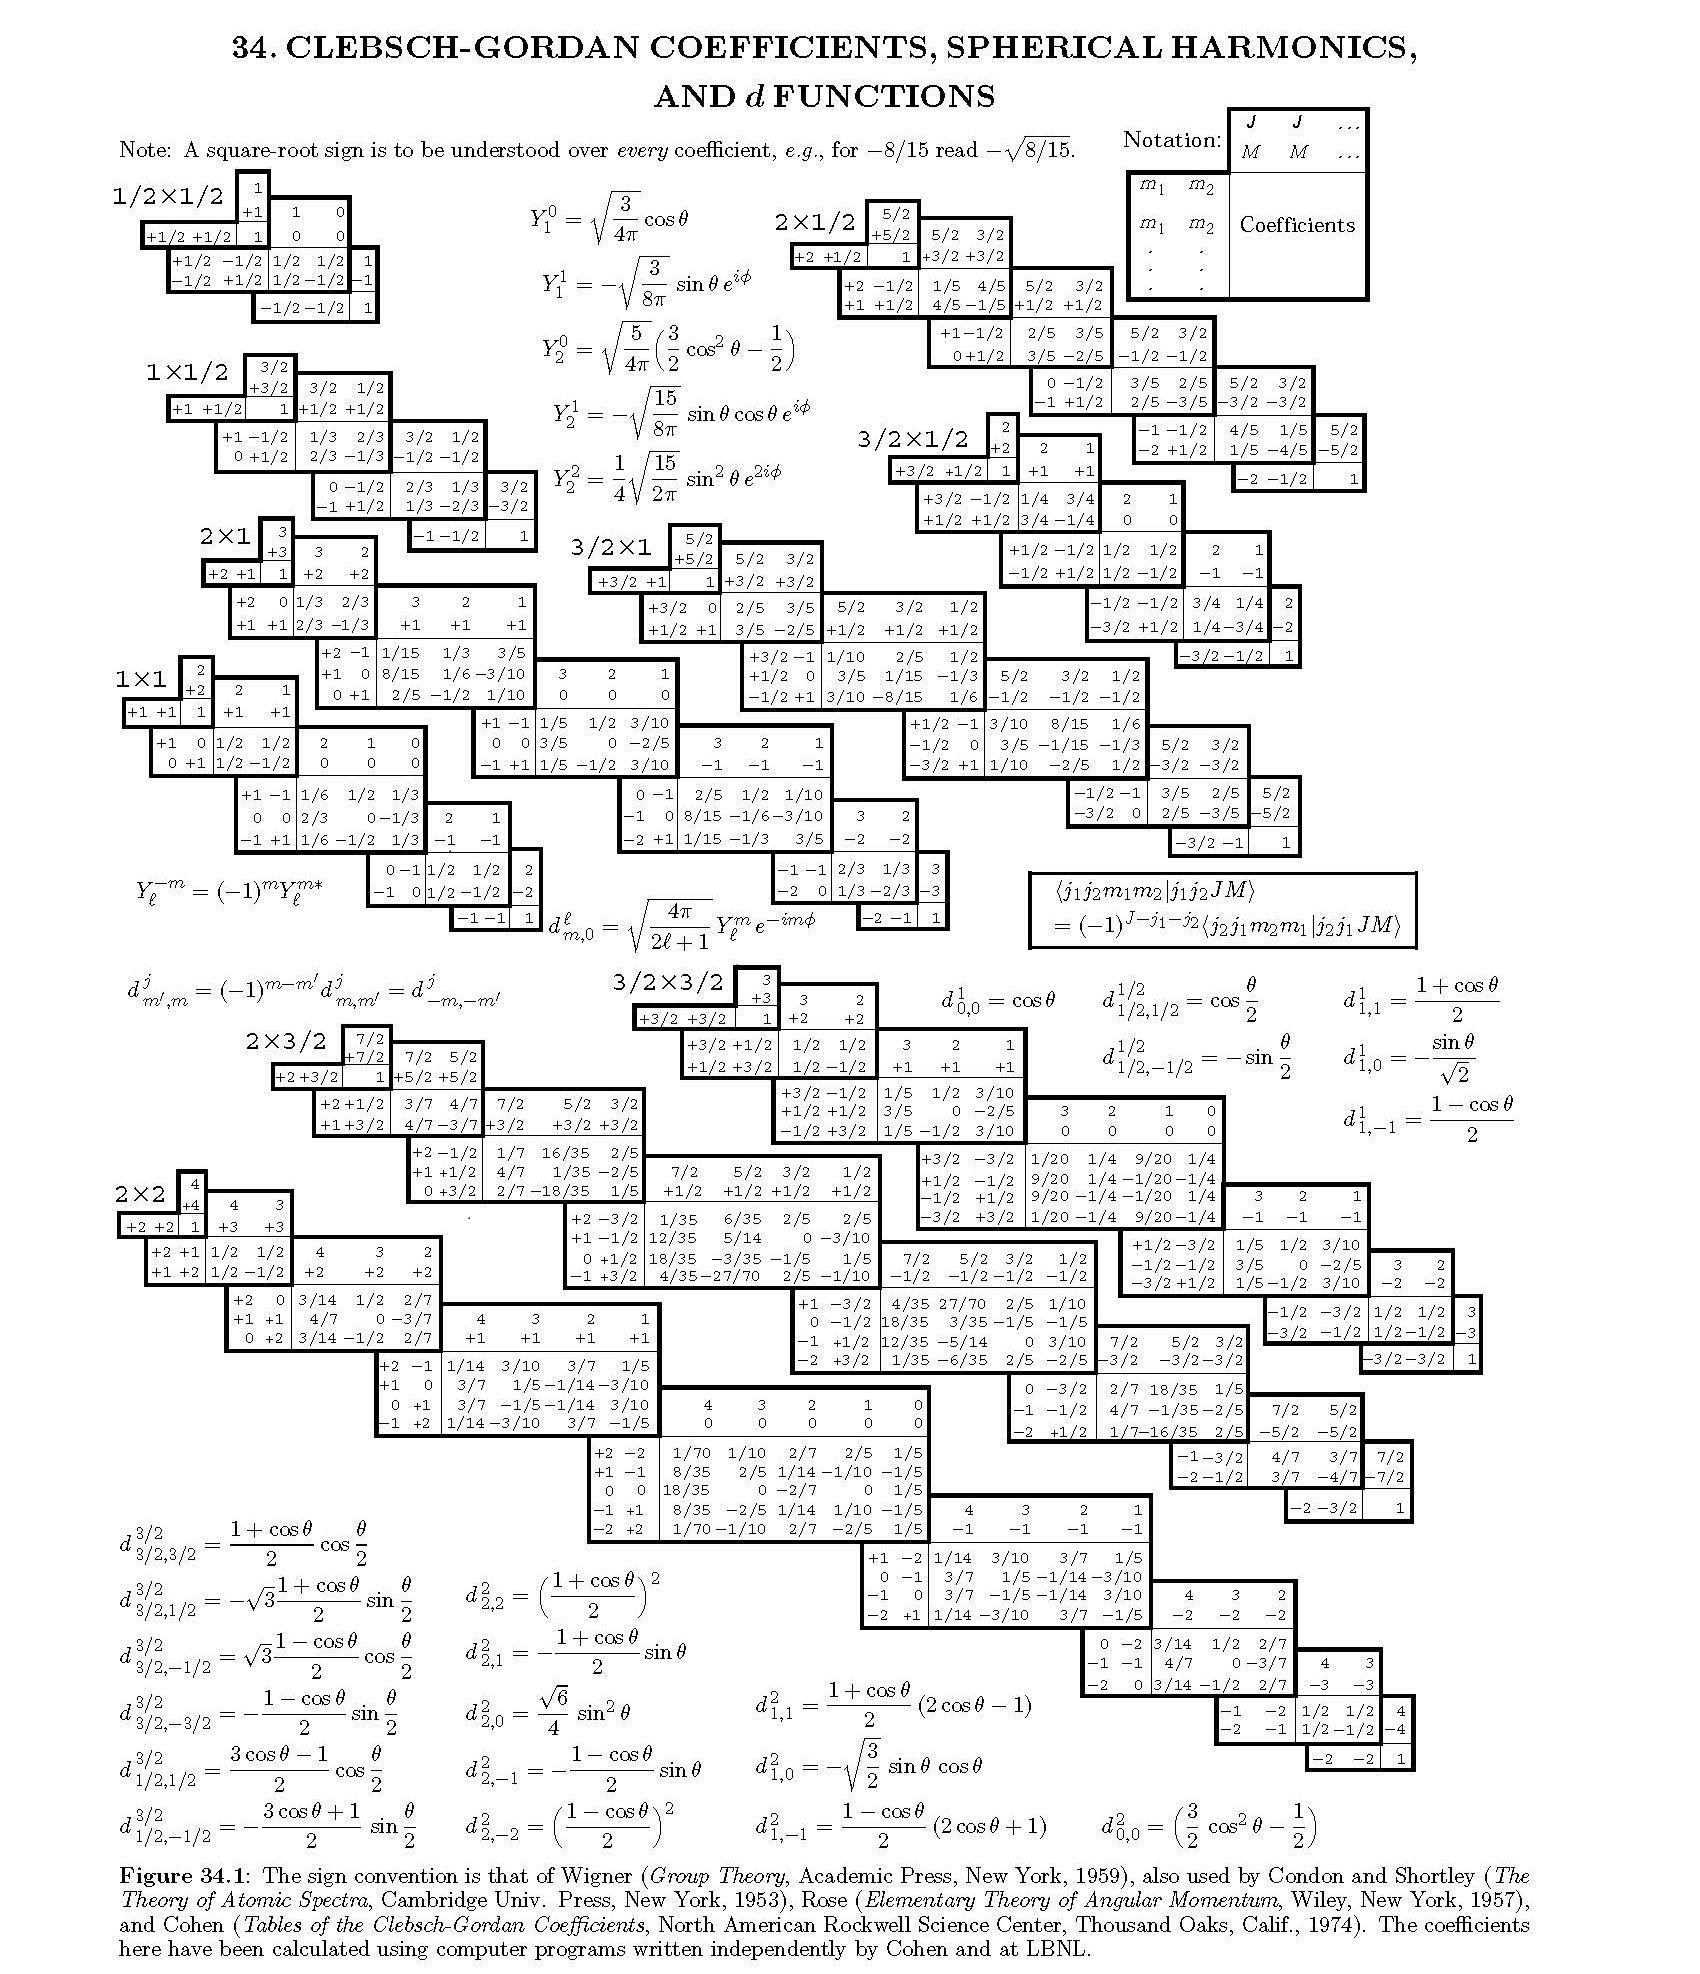
\includegraphics[width=\textwidth]{figure/CGcoefficent.jpg}
    \caption{C-G系数表}
    \label{fig5:CGcoefficient}
\end{figure}

 
\chapter{氢原子}

    \begin{introduction}
    \item 氢原子波函数与能量本征值的求解
\end{introduction}
    \section{Schrodinger方程的求解}
        \subsection{氢原子问题的单体化}
            本章节的任务是求解氢原子的波函数和能量本征值。首先我们观察体系:氢原子是由一个质子和一个质子组成的简单两粒子系统,质子与电子之间存在静电势场\footnote{在不同单位制下静电势能的系数有所不同,因此这里同一用一个抽象的$\kappa$代替。}$V(|\vec{r_p}-\vec{r_e}|)=-\frac{\kappa}{|\vec{r_p}-\vec{r_e}|}$,其中$\vec{r_p}$是质子的位移,$\vec{r_e}$是电子的位移。考虑体系的Hamiltonian:
            \begin{equation}
                 \hat{H}=-\frac{\hbar^2}{2m_p}\nabla^2-\frac{\hbar^2}{2m_e}\nabla^2-\frac{\kappa}{|\vec{r_p}-\vec{r_e}|}
            \end{equation}
            
            可以发现,虽然氢原子的Hamiltonian不含时间,因此我们可以用定态方程$\hat{H}\psi=E\psi$描述,但是由于势能项存在耦合项,因此不能直接分离变量。在大学物理课中,我们已经知道了如何处理两体问题:即将两粒子的运动分解为两粒子整体的平动以及两粒子间的相对运动。我们可以迁移到氢原子的体系中来,于是我们引入了以下两个矢量:
            \begin{align}
                \begin{split}
                    \vec{R}=&\frac{m_p\vec{r_p}+m_e\vec{r_e}}{m_p+m_e}=\frac{m_p\vec{r_p}+m_e\vec{r_e}}{M}\equiv (X,Y,Z)\\
                    \vec{r}=&\vec{r_e}-\vec{r_p}
                \end{split}
            \end{align}
            
            其中$M=m_p+m_e$,是两粒子的总质量;并且由定义,我们知道$\vec{r}$代表电子相对于质子的相对位矢,$\vec{R}$代表质心运动的位矢。联立两式,我们可以用$\vec{R},\vec{r}$来表示$\vec{r_p},\vec{r_e}$:
            \begin{align}\label{equ6:transformformotion}
                \begin{split}
                    \vec{r_p}=\vec{R}-\frac{m_e}{M}\vec{r}\\
                    \vec{r_e}=\vec{R}+\frac{m_p}{M}\vec{r}
                \end{split}
            \end{align}
            
            此外对于相对运动而言,我们往往会定义一个约化质量$\mu$,它的定义如下:
            \begin{align}
                \begin{split}
                    \mu=&\frac{m_pm_e}{m_p+m_e}=\frac{m_pm_e}{M}\\
                    \frac{1}{\mu}=&\frac{1}{m_p}+\frac{1}{m_e}
                \end{split}
            \end{align}
                
            现在考虑定态方程:
            \begin{equation}\label{equ6:stationaryequA}
                (-\frac{\hbar^2}{2m_p}\nabla^2-\frac{\hbar^2}{2m_e}\nabla^2-\frac{\kappa}{|\vec{r_p}-\vec{r_e}|})\psi(\vec{r_p},\vec{r_e})=E_T\psi(\vec{r_p},\vec{r_e})
            \end{equation}
            
            我们的目标是将上述定态方程变成只含有变量$\vec{R},\vec{r}$的方程,首先我们考虑动能项分量\footnote{因为分量是标量,较好容易做导数计算}的一阶偏导\footnote{根据\ref{equ6:transformformotion}式,我们知道$\vec{R},\vec{r}$中一定含有$x_p,x_e$,因此我们可以将$\psi$对$x_p,x_e$的偏导写成类似全微分的形式}:
            \begin{align}
                \begin{split}
                    \frac{\partial\psi(\vec{R},\vec{r})}{\partial x_p}=&\frac{\partial\psi(\vec{R},\vec{r})}{\partial X}\frac{\partial X}{\partial x_p}+\frac{\partial\psi(\vec{R},\vec{r})}{\partial x}\frac{\partial x}{\partial x_p}\\
                    =& \frac{m_p}{M}\frac{\partial\psi(\vec{R},\vec{r})}{\partial X}-\frac{\partial\psi(\vec{R},\vec{r})}{\partial x}\\
                    \frac{\partial\psi(\vec{R},\vec{r})}{\partial x_e}=&\frac{\partial\psi(\vec{R},\vec{r})}{\partial X}\frac{\partial X}{\partial x_e}+\frac{\partial\psi(\vec{R},\vec{r})}{\partial x}\frac{\partial x}{\partial x_e}\\
                    =& \frac{m_e}{M}\frac{\partial\psi(\vec{R},\vec{r})}{\partial X}+\frac{\partial\psi(\vec{R},\vec{r})}{\partial x}
                \end{split}
            \end{align}
            
            再得到一阶导数的形式以后,利用算子的计算规律,我们可以得到二阶偏微分算符的形式:
            \begin{align}\label{equ6:transA}
                \begin{split}
                    \frac{\partial^2}{\partial x_p^2}=&\Big(\frac{m_p}{M}\frac{\partial }{\partial X}-\frac{\partial}{\partial x}\Big)\Big(\frac{m_p}{M}\frac{\partial }{\partial X}-\frac{\partial}{\partial x}\Big)\\
                    =&\frac{m_p^2}{M^2}\frac{\partial^2}{\partial X^2}-\frac{2m_p}{M}\frac{\partial^2}{\partial X\partial x}+\frac{\partial^2}{\partial x^2}\\
                    \frac{\partial^2}{\partial x_e^2}=&\Big(\frac{m_e}{M}\frac{\partial }{\partial X}+\frac{\partial}{\partial x}\Big)\Big(\frac{m_e}{M}\frac{\partial }{\partial X}+\frac{\partial}{\partial x}\Big)\\
                    =&\frac{m_e^2}{M^2}\frac{\partial^2}{\partial X^2}+\frac{2m_e}{M}\frac{\partial^2}{\partial X\partial x}+\frac{\partial^2}{\partial x^2}
                \end{split}
            \end{align}
            
            观察\ref{equ6:transA}式,我们可以通过加减消元消去中间项$\frac{\partial^2}{\partial X\partial x}$:
            \begin{align}
                \begin{split}
                    \frac{1}{m_p}\frac{\partial^2}{\partial x_p^2}+\frac{1}{m_e}\frac{\partial^2}{\partial x_e^2}=& \frac{m_p+m_e}{M^2}\frac{\partial^2}{\partial X^2}+\Big(\frac{1}{m_p}+\frac{1}{m_e}\Big)\frac{\partial^2}{\partial x^2}\\
                    =&\frac{1}{M}\frac{\partial^2}{\partial X^2}+\frac{1}{\mu}\frac{\partial^2}{\partial x^2}
                \end{split}
            \end{align}
            
            同理,其它分量也有类似的关系,于是:
            \begin{equation}
                \frac{1}{m_p}\nabla_p^2+\frac{1}{m_e}\nabla_e^2=\frac{1}{M}\nabla_R^2+\frac{1}{\mu}\nabla_r^2
            \end{equation}
            
            代入定态方程\ref{equ6:stationaryequA}式,我们可以得到:
            \begin{equation}
                -\Big(\frac{\hbar^2}{2M}\nabla_R^2+\frac{\hbar^2}{2\mu}\nabla_r^2+\frac{\kappa}{r}\Big)\psi(\vec{R},\vec{r})=E_T\psi(\vec{R},\vec{r})
            \end{equation}
            
            可以发现,上式是可以进行分离变量的,不妨令$\psi(\vec{R},\vec{r})=\phi(\vec{R})\psi(\vec{r})$,同时假设分离变量以后等号两边等于常数-$E_C$\footnote{这里取负号是为了方程形式上好看},于是则有关系:
            \begin{align}
                \begin{split}
                    -\frac{\hbar^2}{2M}\nabla_R^2\phi(\vec{R})=E_C\phi(\vec{R})\\
                    \Big(-\frac{\hbar^2}{2\mu}\nabla_r^2-\frac{\kappa}{r}\Big)\psi(\vec{r})=E\psi(\vec{r})
                \end{split}
            \end{align}
            
            其中$E=E_T-E_C$。可以发现,关于$\vec{R}$的本征方程和自由粒子的Schrodinger方程形式一样,因此我们可以写出$\phi(\vec{R})$的形式为:
            \begin{equation}
                \phi(\vec{R})=(2\pi\hbar)^{-\frac{3}{2}}\exp{\frac{i\vec{P}\cdot \vec{R}}{\hbar}}
            \end{equation}
            
            于是问题转化为了求解氢原子相对运动的本征值问题。
        \subsection{球坐标系下的本征方程}
        
        回顾氢原子质子与电子间相互作用的本征方程:
        \begin{equation}\label{equ6:stationaryequB}
            \Big(-\frac{\hbar^2}{2m_e}\nabla_r^2-\frac{\kappa}{r}\Big)\psi(\vec{r})=E\psi(\vec{r})
        \end{equation}
        
        由于质子质量远大于电子质量(相差4个数量级),因此我们可以用电子质量代替约化质量$mu$,即$\mu=\frac{m_em_p}{m_e+m_p}\sim \frac{m_em_p}{m_p}=m_e$。同时,如果我们将氢原子核看作零点,那么势能项只与到原点的矢量有关(即可以表示成$V(\vec{r})$),一般来说,在这种情况下我们都会采用球坐标系作为参考系。
        
        球坐标系是极坐标系拓展到三维的一种情况,对于三维空间上的任意一个点P,我们采用原点到P点的距离$r$,原点到P点的连线与正z轴之间的天顶角$\theta$以及原点到点P的连线在xy平面的投影线与正x轴之间的方位角$\varphi$(可以参考图\ref{fig:spherecoordinate})。三个基底的变化范围定义为:$r\in[0,+\infty],\theta\in[0,\pi],\varphi\in[0,2\pi]$
        
        \begin{figure}[H]
            \centering
            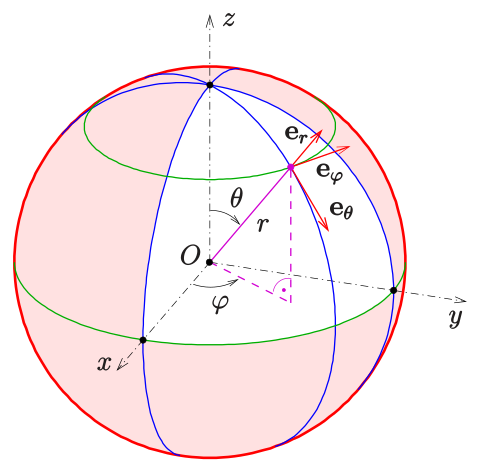
\includegraphics[width=0.5\textwidth]{figure/sphere.png}
            \caption{球坐标系的基底选择}
            \label{fig:spherecoordinate}
        \end{figure}
        
        我们需要将Laplace算符改写成球坐标系下的形式,因此我们要对算符进行坐标变换。根据示意图,我们可以直接写出直角坐标与球坐标间的变换关系:
        \begin{align}
            \begin{split}
                x=&rsin\theta cos\varphi\\
                y=&rsin\theta sin\varphi\\
                z=&rcos\theta
            \end{split}
        \end{align}
        
        代入Laplace算子中我们可以知道其在球坐标系下的形式\footnote{具体计算可以参考田光善的量子力学讲义Ch0}:
        \begin{equation}
            \nabla^2=\frac{1}{r^2}\frac{\partial}{\partial r}\Big(r^2\frac{\partial}{\partial  r}\Big)+\frac{1}{r^2\sin{\theta}}\frac{\partial}{\partial \theta}\Big(\sin{\theta}\frac{\partial}{\partial \theta}\Big)+\frac{1}{r^2\sin{\theta}}\frac{\partial^2}{\partial\varphi^2}
        \end{equation}
        
        代入本征方程\ref{equ6:stationaryequB}式,可以得到:
        \begin{equation}
            \frac{\hbar^2}{2m_e}\Big(\frac{1}{r^2}\frac{\partial}{\partial r}\Big(r^2\frac{\partial\psi}{\partial  r}\Big)+\frac{1}{r^2\sin{\theta}}\frac{\partial}{\partial \theta}\Big(\sin{\theta}\frac{\partial\psi}{\partial \theta}\Big)+\frac{1}{r^2\sin^2{\theta}}\frac{\partial^2\psi}{\partial\varphi^2}\Big)+V\psi =E\psi
        \end{equation}
        
        可以发现,由于$V=V(r)$,因此上述方程是可以分离变量的。令$\psi(r,\theta,\varphi)=R(r)Y(\theta,\varphi)$,可以得到:
        \begin{equation}
            \frac{\hbar^2}{2m_e}\Big(\frac{Y}{r^2}\frac{\partial }{\partial r}\Big(r^2\frac{\partial R}{\partial  r}\Big)+\frac{R}{r^2\sin{\theta}}\frac{\partial }{\partial \theta}\Big(\sin{\theta}\frac{\partial Y}{\partial \theta}\Big)+\frac{R}{r^2\sin^2{\theta}}\frac{\partial^2 Y}{\partial\varphi^2}\Big)+(V-E)RY=0
        \end{equation}
        
        等号两边同时除以RY,并且同时乘以$-\frac{2m_e}{\hbar^2}$,可得:
        \begin{equation}
            \Big\{\frac{1}{R}\frac{d}{dr}\Big(r^2\frac{dR}{dr}\Big)-\frac{2m_e}{\hbar^2}(V-E)\Big\}+\frac{1}{Y}\Big\{\frac{1}{\sin{\theta}}\frac{d}{d\theta}\Big(\sin{\theta}\frac{dY}{d\theta}\Big)+\frac{1}{\sin^2{\theta}}\frac{d^2Y}{d\varphi^2}\Big\}=0
        \end{equation}
        
        按照分离变量法的步骤,两个大括号相等当且仅当这两个大括号等于一个常数,我们令常数为$l(l+1)$\footnote{为什么常数的形式是$l(l+1)$将在后续内容中解释},则我们可以得到两个本征方程:
        
        \begin{align}
            \begin{split}
                \frac{1}{R}\frac{d}{dr}\Big(r^2\frac{dR}{dr}\Big)-\frac{2m_e}{\hbar^2}(V-E)=&l(l+1)\\
                \frac{1}{Y}\Big\{\frac{1}{\sin{\theta}}\frac{d}{d\theta}\Big(\sin{\theta}\frac{dY}{d\theta}\Big)+\frac{1}{\sin^2{\theta}}\frac{d^2Y}{d\varphi^2}\Big\}=&-l(l+1)
            \end{split}
        \end{align}
        \subsection{角动量方程的求解}
            本节我们考虑$Y(\theta,\varphi)$对应的本征方程:
            \begin{equation}
                \frac{1}{Y}\Big\{\frac{1}{\sin{\theta}}\frac{d}{d\theta}\Big(\sin{\theta}\frac{dY}{d\theta}\Big)+\frac{1}{\sin^2{\theta}}\frac{d^2Y}{d\varphi^2}\Big\}=-l(l+1)
            \end{equation}

            等号两边同时乘以$Y\sin^2{\theta}$可以得到:
            \begin{equation}
                \sin{\theta}\frac{d}{d\theta}\Big(\sin{\theta}\frac{dY}{d\theta}\Big)+\frac{d^2Y}{d\varphi^2}+l(l+1)\sin{\theta}Y=0
            \end{equation}
            
            我们发现该式同样能够分离变量:$Y(\theta,\varphi)=\Theta(\theta)\Phi(\varphi)$,代入可得:
            \begin{equation}
                \Phi\sin{\theta}\frac{d}{d\theta}\Big(\sin{\theta}\frac{d\Theta}{d\theta}\Big)+\Theta\frac{d^2\Phi}{d\varphi^2}+l(l+1)\sin{\theta}\Theta\Phi=0
            \end{equation}
            
            等号两边同时除以$\Theta\Phi$,可得:
            \begin{equation}
                \frac{\sin{\theta}}{\Theta}\frac{d}{d\theta}\Big(\sin{\theta}\frac{d\Theta}{d\theta}\Big)+l(l+1)\sin{\theta}+\frac{1}{\Phi}\frac{d^2\Phi}{d\varphi^2}=0
            \end{equation}
            
            自然我们可以得到两个本征方程,设此时的分离常数为$m^2$,那么:
            \begin{align}
                \begin{split}
                    \frac{\sin{\theta}}{\Theta}\frac{d}{d\theta}\Big(\sin{\theta}\frac{d\Theta}{d\theta}\Big)+&l(l+1)\sin{\theta}=m^2\\
                    \frac{1}{\Phi}\frac{d^2\Phi}{d\varphi^2}=-m^2
                \end{split}
            \end{align}
            
            先看$\Phi(\phi)$的方程,这是一个简单的微分方程,经过简单计算,我们可以得到通解为:
            \begin{equation}
                \Phi(\varphi)=Ae^{im\varphi}
            \end{equation}
            
            这里本来有两个解$e^{im\varphi},e^{-im\varphi}$的,但是由于$m$的取值既可以取正也可以取负,因此这两个解是线性相关的,只取一个就可以了。考虑边界条件,由于在球坐标的定义下,当$\varphi$转过$2\pi$角度时,粒子应该回到同一点,因此边界条件应该是周期条件:$\Phi(\varphi+2\pi)=\Phi(\varphi)$,因此:
            \begin{equation}
                e^{im\varphi}=e^{im(\varphi+2\pi)}\Rightarrow e^{2\pi im}=1,m=0,\pm 1,\dots
            \end{equation}
            
            归一化常数$A$可以通过$\Theta$的归一化可以求得:
            \begin{equation}
                \int_0^{2\pi}\Phi^*(\varphi)\Phi(\varphi)d\varphi=\int_0^{2\pi}A e^{im\varphi}\cdot Ae^{im\varphi}d\varphi=2\pi A^2=1
            \end{equation}
            
            于是可以得到:$A=\frac{1}{\sqrt{2\pi}}$,于是解的形式:
            \begin{equation}
                \Phi(\varphi)=\frac{1}{\sqrt{2\pi}}e^{im\varphi}
            \end{equation}
            
            下面讨论有关$\Theta(\theta)$的方程:
            \begin{equation}
                \frac{1}{\sin{\theta}}\frac{d}{d\theta}\Big(\sin{\theta}\frac{d\Theta}{d\theta}\Big)+\Big(l(l+1)-\frac {m^2}{\sin^2{\theta}}\Big)
            \end{equation}
            
            在附录B中我们介绍了Sturm-Liouville方程在Hilbert空间中具有重要意义。上式对比Sturm-Liouville方程的形式:
            \begin{equation}
                \frac{d}{dx}\Big(p(x)\frac{dy}{dx})+(q(x)+\lambda)x=0
            \end{equation}
            
            我们可以发现形式已经大致相似了,唯一有问题的地方就是三角函数,于是我们作坐标变换:$z=\cos{\theta},z\in \mathbb{R}[-1,1];P(z)=\Theta(\theta)$,则:
            \begin{align}
                \begin{split}
                    \frac{d\Theta}{d\theta}=&\frac{dP}{dz}\cdot \frac{dz}{\theta}=\frac{dP}{dz}\sin{\theta}\\
                    \sin^2{\theta}=&1-z^2
                \end{split}
            \end{align}
            
            代入可得:
            \begin{equation}
                \frac{d}{dz}\Big((1-z^2)\frac{dP}{dz}\Big)+\Big(l(l+1)-\frac{m^2}{1-z^2}\Big)P=0
            \end{equation}
            %补充Sturm-Liouville方程具有的性质
        \subsection{径向方程的求解}
        
        现在考虑径向方程:
        \begin{equation}
            \frac{1}{R}\frac{d}{dr}\Big(r^2\frac{dR}{dr}\Big)-\frac{2m_e}{\hbar^2}(V-E)=l(l+1)
        \end{equation}
        
        我们同样考虑将其转换成Sturm-Liouville方程的形式。等号两边同乘$\frac{R}{r^2}$,可以得到:
        \begin{equation}
            \frac{1}{r^2}\frac{d}{dr}\Big(r^2\frac{dR}{dr}\Big)-\Big[\frac{2m}{\hbar^2}\Big(\frac{Ze^2}{r}-E\Big)+\frac{l(l+1)}{r^2}\Big]R=0
        \end{equation}
        
        由于电子和核子之间的相互作用是既有吸引也有排斥的,因此我们需要对E的正负号进行分类讨论。如果E<0,此时电子和核子之间以吸引力为主,较为稳定,不会发生电离;当E>0时,此时氢原子会发生电离,此时电子会遵循自由粒子的运动情况。在一般情况下,我们还是研究稳定的体系,因此在这里E<0。求解是类似的思路,首先我们希望通过去量纲化得到更为普遍的方程形式。


\chapter{变分法}

    \begin{introduction}
    \item 变分法的基本原理
    \item 例子:谐振子与四次势
    \item 线性变分法
\end{introduction}
从本章开始,我们将会介绍两种Schrodinger方程的近似方法,即微扰理论和变分法。微扰理论基于已经有精确解的Schrodinger方程,我们将实际体系的Hamiltonian拆分成精确解对应的Hamiltonian和所谓的微扰Hamiltonian,后者在量级上是比前者作用小很多的。这种处理问题的方式是非常“物理”的:即我们突出物理模型的主要性质,在此基础上,我们再引入近似项,由此来考虑物理模型更“精细”的结构。但是问题也是很明显的,即必须要将体系的Hamiltonian分解为某个可以精确求解的Hamiltonian和某个微扰Hamiltonian的和。但是在很多体系中是难以拆分的;同时在后面我们可以发现,微扰法在考虑高阶波函数与能量近似时计算非常复杂。本节介绍的变分法是量子化学中更为常见的近似方法。
\section{变分法的基本原理}
所谓变分法,简单来说就是求解某一个泛函的极值。求解泛函的方法有很多种,在量子化学中,我们通常采用一种叫Ritzs变分法的方法。这类变分法的基本思想基于以下不等式:任意给定一个well-behaved的态$|\phi\rangle$(我们称之为试探变分函数,trial variation function),都有\footnote{可以发现,试探函数$|\phi\rangle$的要求不高,只需要满足体系的边界条件即可,因此如果选择得当,其收敛速度远远比精确波函数快}:
\begin{equation}\label{equ9:variationequ}
    \frac{\langle \phi|\hat{H}|\phi\rangle}{\langle \phi|\phi\rangle}\geq E_0
\end{equation}

其中$\hat{H}$是体系的Hamiltonian,$E_0$是体系的基态能量。可以看出对于态空间任意的态,其能量的平均值一定不小于基态能量,下面给出证明。

设体系的本征方程为:
\begin{equation}
    \hat{H}|\psi_n\rangle=E_n|\psi_n\rangle
\end{equation}

自然,$|\phi\rangle$可以写成本征态的线性组合:
\begin{equation}
    |\phi\rangle=\sum_n c_n|\psi_n\rangle
\end{equation}

于是则有
\begin{align}
    \begin{split}
        \langle \phi|\hat{H}|\phi\rangle=&\sum_{m,n}c_m^*c_n\langle\phi_m|\hat{H}|\phi_n\rangle\\
        =& \sum_{m,n}c_mc_n E_n \delta_{mn}\\
        =& \sum_n |c_n|^2 E_n \\
        \geq& \sum_n |c_n|^2 E_1 \\
        =& E_1\langle \phi|\phi\rangle
    \end{split}
\end{align}

移项即可得\ref{equ9:variationequ}式。进一步,如果$|\phi\rangle$含有参数$\alpha$,那么显然最接近基态能量$E_0$的能量平均值$\langle E(\alpha^*)\rangle$应该满足:
\begin{equation}
    \left.\frac{\partial \langle E(\alpha)\rangle}{\partial \alpha_i}\right|_{\alpha=\alpha^*}=0
\end{equation}

这样我们就可以得到该函数下最好的基态描述。如果试探函数选择得当,那么变分法可以得到非常精确的结果。
\section{一个简单的例子}

\section{线性变分法}
上面是一些简单的例子,在实际研究中,试探函数的建立没有那么容易。由于我们希望试探函数的建立是基于一定的物理的,于是往往会将试探函数$|\phi\rangle$用多个线性无关的实函数$|f_i\rangle$展开来表示,即:
\begin{align}
    \begin{split}
        |\phi\rangle=\sum_{i=1}^n c_i|f_i\rangle
    \end{split}
\end{align}

上式代入\ref{equ9:variationequ},可得:
\begin{align}\label{equ9:linearvariation}
    \begin{split}
        \langle E\rangle=&\frac{\langle\phi|\hat{H}|\phi\rangle}{\langle\phi|\phi\rangle}\\
        =&\frac{\sum_{i,j}^nc_ic_j\langle f_i|\hat{H}|f_j\rangle}{\sum_{i,j}^n c_ic_j\langle f_i|f_j\rangle}\\
        \Rightarrow&\langle E\rangle\sum_{i,j}^n c_ic_jS_{ij}=\sum_{i,j}^n c_ic_jH_{ij}
    \end{split}
\end{align}

可以看到,$\langle E\rangle$是含有参数$\{c_i\}$的,于是需要满足:
\begin{equation}
    \frac{\partial \langle E\rangle}{\partial c_k}=0,k=1,2,\dots,n
\end{equation}

于是我们考虑对\ref{equ9:linearvariation}式进行隐函数求偏导:
\begin{equation}\label{equ9:A}
     \frac{\partial\langle E\rangle}{\partial c_k}\sum_{i,j}^n c_ic_jS_{ij}+\langle E\rangle\frac{\partial}{\partial c_k}\Big(\sum_{i,j}^n c_ic_jS_{ij}\Big)=\frac{\partial}{\partial c_k}\Big(\sum_{i,j}^n c_ic_jH_{ij}\Big)
\end{equation}

其中$S_{ij}=\langle f_i|f_j\rangle$,称为重叠积分\footnote{为了保持连贯性,因此我这里仍然使用Dirac符号,但是实际我们计算的时候是采用积分形式的};$H_{ij}=\langle f_i|\hat{H}|f_j\rangle$

由于$S_{ij}$是常数,因此上式中的几项都可以化简:
\begin{align}
    \begin{split}
        \frac{\partial}{\partial c_k}\Big(\sum_{i,j}^n c_ic_jS_{ij}\Big)=&\sum_{i,j}^n\frac{\partial}{\partial c_k}( c_ic_j)S_{ij}\\
        =&\sum_{i,j}^n(\frac{\partial c_i}{\partial c_k}c_j+\frac{\partial c_j}{\partial c_k}c_i)S_{ij}
    \end{split}
\end{align}

由于:
\begin{equation}
    \frac{\partial c_i}{\partial c_j}=\delta_{ij}
\end{equation}

于是:
\begin{equation}
    \sum_{i,j}^n(\frac{\partial c_i}{\partial c_k}c_j+\frac{\partial c_j}{\partial c_k}c_i)S_{ij}=\sum_j c_jS_{kj}+\sum_i c_i S_{ik}
\end{equation}

由于$S_{ij}$是一个内积形式,我们根据内积定义,结合内积是实数,可以知道:
\begin{equation}
    \langle f_i|f_j\rangle=(\langle f_j|f_i\rangle)^*=\langle f_j|f_i\rangle
\end{equation}

即:$S_{ij}=S_{ji}$,于是上式可以变为:
\begin{equation}
    \frac{\partial}{\partial c_k}\Big(\sum_{i,j}^n c_ic_jS_{ij}\Big)=\sum_j c_jS_{kj}+\sum_i c_i S_{ik}=2\sum_i c_i S_{ik}
\end{equation}

同理:
\begin{equation}
    \frac{\partial}{\partial c_k}\Big(\sum_{i,j}^n c_ic_jH_{ij}\Big)=\sum_j c_jS_{kj}+\sum_i c_i H_{ik}=2\sum_i c_i H_{ik}
\end{equation}

于是,\ref{equ9:A}式可以化简为:
\begin{equation}\label{equ9:B}
    \sum_i c_iH_{ik}-\langle E\rangle\sum_i c_iS_{ik}=0
\end{equation}

可以看到,上式是一个关于$\{c_i\}$的齐次线性方程组,我们知道,齐次线性方程组有非平凡解当且仅当系数行列式为0,即满足:
\begin{equation}
    \det(H-\langle E\rangle S)=0
\end{equation}

通过求解行列式我们可以得到$\langle E\rangle$的前n个解:$\langle E\rangle_1,\langle E\rangle_2,\dots,\langle E\rangle_n$,可以证明体系的能量与$\langle E\rangle$的关系为:
\begin{equation}
    E_1\leq \langle E\rangle_1, E_2\leq \langle E\rangle_2,\dots, E_n\leq \langle E\rangle_n
\end{equation}

因此,线性变分法的结果就是给出了体系前n级能量的上界(upper bound)。如果我们想要获得体系的更多级能量,在构造试探函数的时候就要用更多数量的函数$|f_i\rangle$展开,同时更完备的函数集可能会提高求解能量的精确性,但是可惜的是,由于计算机算力的限制,我们往往只能使用有限的基函数来代表完备集。

特别的,如果$\{|f_i\rangle\}$是正交的,那么$S_{ij}=\langle f_i|f_j\rangle=\delta_{ij}$。因此\ref{equ9:B}式可以表示为:
\begin{equation}
     \sum_i c_iH_{ik}-\langle E\rangle c_k=0
\end{equation}

这也是一个线性齐次方程组,我们可以将其展开写成:
\begin{align}
    \begin{split}
        H_{11}c_1+H_{12}c_2+\dots+H{1n}c_n=&\langle E\rangle c_1\\
        H_{21}c_1+H_{22}c_2+\dots+H{2n}c_n=&\langle E\rangle c_2\\
        \dots\dots\dots\dots\dots\\
        H_{n1}c_1+H_{n2}c_2+\dots+H{nn}c_n=&\langle E\rangle c_n
    \end{split}
\end{align}

可以明显看出,这个方程组可以写成本征方程的形式,即:
\begin{equation}
    Hc=\langle E\rangle c
\end{equation}

其中$H=\begin{pmatrix} H_{11}&H_{12}&\dots&H_{1n}\\H_{21}&H_{22}&\dots&H_{2n}\\ \dots&\dots&\dots&\dots\\H_{n1}&H_{n2}&\dots&H_{nn}\end{pmatrix},c=\begin{pmatrix}c_1\\c_2\\ \vdots\\c_n\end{pmatrix}$

对于计算机来说,更好的求解方程组的手段是求解矩阵方程。因此我们换一种方式理解线性变分法的求解。令上述本征方程的n个本征值为$W_1,W_2,\dots,W_n$,本征态为$c^{i}$\footnote{注意,这是一个列矢量},那么本征方程自然可以表达为:
\begin{equation}
    Hc^{(i)}=W_ic^{(i)},i=1,2,\dots,n
\end{equation}

显然,我们可以通过一个矩阵方程将上面n个本征方程组合并:
\begin{equation}
    HC=CW
\end{equation}

其中:
$C=\begin{pmatrix}c_{1}^{(1)}&c_{1}^{(2)}&\dots&c_{1}^{(n)}\\c_{2}^{(1)}&c_{2}^{(2)}&\dots&c_{2}^{(n)}\\ \dots&\dots&\dots&\dots\\c_{n}^{(1)}&c_{n}^{(2)}&\dots&c_{n}^{(n)}\end{pmatrix},W=\begin{pmatrix}W_1&\quad&\quad&\quad\\ \quad&W_2&\quad&\quad \\ \quad&\quad&\ddots&\quad\\ \quad &\quad&\quad&W_n \end{pmatrix}$。组成矩阵C的向量集$\{c^{(i)}\}$是正交的,因此C一定可逆。如果H是Hermitian,则C是一定是幺正矩阵,那么矩阵方程就可以看作是将H矩阵对角化的过程:
\begin{equation}
    W=C^\dagger H C
\end{equation}

实际上,求解行列式的本质在于求解多项式的根,其坏处在于,如果对多项式的系数作微小的改变,最后的结果会相差很大。这就需要计算机对于多项式根的求解有非常高的灵敏度;而矩阵的对角化问题不仅抗扰动能力强,同时在数值计算中已经有比较成熟的处理方法了。因此,目前我们主要采取后者作为分析的主要方法。
    
\chapter{定态微扰论}

    %CH7 定态微扰论
\begin{introduction}
    \item 非简并微扰论
    \item 简并微扰论
    \item 氢原子的$Starks$效应
    \item 氢原子的精细结构
    \item $Zeeman$效应
\end{introduction}
\section{微扰论概述}
从本章开始,我们开始考虑另一种对$Schrodinger$方程的近似求解。从之前的内容中已经知道,即使是类似氢原子那样非常简单的势场,最终的求解仍然是非常复杂的,我们对$He$元素的方程求解已经无能为力,更不用说我们去讨论实际科研中运用到的多体的$Schrodinger$方程。因此寻找一种近似求解的方法是非常重要的。

对于量子力学的定态$Schrodinger$方程,我们可以将$Hamiltonian$写作:
\begin{equation}
    \hat{H}=\hat{H_0}+\hat{H'}
\end{equation}

其中$\hat{H_0}$是可精确求解的$Hamiltonian$,$\hat{H'}$是相对于$\hat{H_0}$上的微扰,它的效应相比$\hat{H_0}$非常微小。如果$\hat{H'}$不含时间,则我们称此时处理的问题为定态微扰问题。本章我们讨论的问题是考虑$\hat{H'}$不含时间的情况下,能级和态受到的修正情况。
    \subsection{微扰方程与其约束条件}
    我们考虑的前提是本征方程:
    \begin{equation}\label{equ7:weirao}
        \hat{H}|\psi \rangle =E |\psi \rangle
    \end{equation}
    
    考虑到一般情况下微扰算符$\hat{H'}$的量级为$\hat{H_0}$的1\%左右,为了让微扰效应突出,我们可以将微扰算符看作一个实数小量$\varepsilon$和一个量级和$\hat{H_0}$相似的算符$\hat{W}$的乘积:
    \begin{equation} \label{equ7:suanfu}
        \hat{H'}=\varepsilon \hat{W}
    \end{equation}
    
    于是我们便可以将$\hat{H}$看作$\varepsilon$的泛函。由于$E,|\psi \rangle$是含有微扰的算符作用后得到的总能量和态矢量,因此我们可以想象,$E,|\psi \rangle$应该是含有变量$\varepsilon$的。数学上我们便可以对其进行幂级数展开
    \footnote{事实上,这里的幂级数展开并没有讨论两个函数的收敛性,而这点实际上非常重要,但在本文中不予考虑}:
    
    \begin{align} \label{equ7:mijishu}
        \begin{split}
            E=& E^{(0)}+E^{(1)}\varepsilon+E^{(2)}\varepsilon^2+\cdots\\
            |\psi\rangle=&|0\rangle+\varepsilon|1\rangle+\varepsilon^2|2\rangle+\cdots
        \end{split}
    \end{align}
    
    将式\eqref{equ7:mijishu}、\eqref{equ7:suanfu}代入 \eqref{equ7:weirao},可得:
        \begin{align}
            \begin{split}
                (\hat{H_0}+\varepsilon\hat{W})(|0\rangle+\varepsilon|1\rangle+\varepsilon^2|2\rangle+\cdots) =\\
                (E^{(0)}+E^{(1)}\varepsilon+E^{(2)}\varepsilon^2+\cdots) (|0\rangle+\varepsilon|1\rangle+\varepsilon^2|2\rangle+\cdots)
            \end{split}
        \end{align}
        
    通过比等号两侧$\varepsilon^0,\varepsilon^1,\varepsilon^2$前的系数,我们可以得到:
            \begin{align}\label{equ:0thpert}
                \hat{H_0}|0\rangle=&E^{(0)}|0\rangle\\ 
            (\hat{H_0}-E^{(0)})|1\rangle+&(\hat{W}-E^{(1)})|0\rangle=0  \label{equ:1stpert}
            \end{align} 
            \begin{equation}
                (\hat{H_0}-E^{(0)})|2\rangle+(\hat{W}-E^{(1)})|1\rangle+E^{(2)}|0\rangle=0 \label{equ:2ndpert}
            \end{equation}
            
            上面三式分别被称为0阶、1阶、2阶微扰方程。在后面的内容中,我们会利用这三个微扰方程求得能量和态的0阶、1阶、2阶微扰项的形式。
            
            在本节的最后,我们希望知道微扰方程的一些约束条件。其中一个重要的约束条件就是:幂级数展开的态$|q\rangle$满足什么性质。根据量子力学的波函数假设,我们知道一个性质“好”的态一定是归一的,于是对于标量积$\langle \psi|\psi \rangle$,我们希望它是归一的,于是考虑它的幂级数展开形式:
            \begin{align}
                 \begin{split}
                     \langle \psi|\psi \rangle=&(\langle0|+\varepsilon\langle1|+\varepsilon^2\langle2|+\cdots)(|0\rangle+\varepsilon|1\rangle+\varepsilon^2|2\rangle+\cdots)+O(\varepsilon^3)\\
                    =&\langle0|0\rangle+\varepsilon(\langle1|0\rangle+\langle0|1\rangle)+\varepsilon^2(\langle2|0\rangle+\langle0|2\rangle+\langle1|1\rangle)+O(\varepsilon^3)
                 \end{split}
            \end{align}
           
            如果只考虑0阶微扰,$|\psi\rangle \approx|0\rangle$,于是$\langle0|0\rangle=1$;如果只考虑到1阶微扰,即$|\psi\rangle \approx|0\rangle+|1\rangle\varepsilon$,那么一定有:$\langle \psi|\psi\rangle\approx\langle0|0\rangle+\varepsilon(\langle1|0\rangle+\langle0|1\rangle)$,则$\langle1|0\rangle+\langle0|1\rangle=0$,即$\langle1|0\rangle=\Bar{\langle0|1\rangle}$。因此要想保证$\langle \psi|\psi \rangle$的归一性,只有$\langle1|0\rangle=\langle0|1\rangle=0$。同理,如果只考虑到2阶微扰,一定满足关系$\langle2|0\rangle=\langle0|2\rangle=-\frac{1}{2}\langle1|1\rangle$。上述关系构成微扰方程约束条件的一部分。
\section{非简并能级的微扰}
本节我们讨论未微扰的$Hamiltonian \hat{H_0}$的一个非简并能级$E^0_n$,它对应的本征态只有一个,即$|\varphi_n\rangle$。根据式\eqref{equ:0thpert},我们知道$|0\rangle$一定是$E_n^0$下的本征态,而对于本征值$E_n^0$来说,本征态只有$|\varphi\rangle$一个,因此$|0\rangle\propto |\varphi_n\rangle$。于是对于0阶微扰,我们可以简单的令:
    \begin{align}
        \begin{split}
            E^0_n=&E^{0}\\
            |\varphi_n \rangle=&|0\rangle
        \end{split}
    \end{align}
    
也就是说,当$\varepsilon\rightarrow0$时,微扰方程退化到无微扰的本征方程。下面开始讨论非简并能级各阶微扰所引起的能量和能级的变化。
      \subsection{1阶修正}  
        根据式\eqref{equ:1stpert},我们考虑左矢$\langle\varphi_n|$的作用,可以得到:
        
        \begin{equation} \label{equ:1stpert_E}
             \langle\varphi_n|\hat{H_0}|1\rangle-\langle\varphi_n|E^{(0)}|1\rangle+\langle\varphi_n|\hat{W}|0\rangle-\langle\varphi_n|E^{(1)}|0\rangle=0 
        \end{equation}

        由于$\langle1|0\rangle=0,|\varphi_n\rangle=|0\rangle$,于是有关系:
        \begin{align}
            \begin{split}
                \langle \varphi| \hat{H_0}|1\rangle=&E^{(0)}\langle1|0\rangle=0\\
               \langle \varphi|E^{(0)}|1\rangle=& E^{(0)}\langle 0|1\rangle=0
            \end{split}
        \end{align}
        
        将上面两式的结果代入\eqref{equ:1stpert_E}中,考虑限制条件$\langle0|0\rangle$,同时等号两边同乘$\varepsilon$使结果保持微扰算符$\hat{H'}$的形式,则有:
        
        \begin{equation}
            E_{1stpertb}=\langle\varphi|\hat{H'}|\varphi\rangle
        \end{equation}

        其中$E_{1stpertb}=\varepsilon E^{(1)}$,被称为能量的一阶微扰项,我们可以发现能量的一阶微扰就等于微扰算符在未微扰态$|\varphi\rangle$下的平均值。
        
        随后我们考虑本征态的一阶微扰近似。我们的思路是利用算符$\hat{H_0}$的其他本征态$|\varphi_m ^0\rangle$
        \footnote{所谓的非简并微扰问题指的是我们研究的能量对应的本征态是非简并的,但是其他能量对应的本征态当然可以是简并的,因此这里我们不失一般性的讨论}作用在1阶微扰方程(即式\eqref{equ:1stpert})上,即可得:
        \begin{equation} \label{equ:1stpert_EE}
             \langle\varphi_m^0|\hat{H_0}|1\rangle-\langle\varphi_m^0|E^{(0)}|1\rangle+\langle\varphi_m^0|\hat{W}|0\rangle-\langle\varphi_m^0|E^{(1)}|0\rangle=0 
        \end{equation}
        由于$\hat{H_0}$是Hermite算符,因此不同本征值的本征态是相互正交的,即:
        $\langle0|\varphi_m^0\rangle=0$;并且根据$\langle\varphi_m^0|\hat{H_0}=\langle\varphi_m^0|E_m^0$,两式代入式\eqref{equ:1stpert_EE},可得:
        \begin{align}
                  (E_m^0-E_n^0) \langle\varphi_m^0|1\rangle=\langle\varphi_m^0|\hat{W}|\varphi_n\rangle \Rightarrow 
               \langle\varphi_m^0|1\rangle=\frac{1}{E_m^0-E_n^0}\langle\varphi_m^0|\hat{W}|\varphi_n\rangle
        \end{align}

        考虑到$\{|\varphi_n^0\}$是态空间上的一组正交归一完备基,于是态空间上任意一个态矢量都可以表示成这组基的线性组合,则有
        \footnote{这里的线性组合本来是对于所有的m的,但是由于$\langle0|1\rangle=0$,因此求和号下就可以撇去m=n的情况}:
        \begin{equation}\label{equ:1stpert_S}
            |1\rangle=\sum_{m\ne n}\langle\varphi_m^0|1\rangle|\varphi_m^0\rangle=
            =\sum_{m \ne n}\frac{\langle\varphi_m^0|\hat{W}|\varphi_n\rangle}{E_m^0-E_n^0}|\varphi_m^0\rangle
        \end{equation}
        
        我们可以看到本征态的1级修正和除了未微扰态$|\varphi_n\rangle$以外的所有本征态有关,如果有效微扰算符在$|\varphi_m^0\rangle$和$|\varphi_n\rangle$之间的矩阵元为0,那么我们可以认为$|\varphi_m^0\rangle$对这个态的贡献为0。一般来说有效微扰算符$\hat{W}$导致的态的耦合程度越强(以矩阵元$\langle\varphi_m^0|\hat{W}|\varphi_n\rangle$ ⟩为判别依据),能级$E_m^0$就越靠近我们要研究的能级$E_n^0$。
        
        \subsection{2阶修正}
        我们用相同的思路可以求解2阶微扰下能量的修正
        \footnote{由于2阶微扰下态的修正项形式较为复杂,同时实际运用中很少用到,因此本笔记不予耗费笔墨于上}
        。考虑左矢$\langle\varphi_n|$对2阶微扰方程式\eqref{equ:2ndpert}的作用:
        \begin{align}
            \begin{split}
                \langle\varphi_n|\hat{H_0}|2\rangle - \langle\varphi_n|E^{(0)}|2\rangle+ \langle\varphi_n|\hat{W}|1\rangle-\langle\varphi_n|E^{(1)}|1\rangle+\langle\varphi_n|E^{(2)}|0\rangle=0
            \end{split}
        \end{align}
        考虑到$|\varphi_n\rangle=|0\rangle,\langle0|1\rangle=0,\langle\varphi_n|\hat{H_0}=\langle\varphi_n E^{0}$,代入上式,则有:
        \begin{equation}
            E^{(2)}=\langle\varphi_n|\hat{W}|1\rangle
        \end{equation}
        
        将式\eqref{equ:1stpert_S}代入上式可得:
        
        \begin{equation}
            E^{(2)}=\sum_{m \ne n}\frac{\langle\varphi_m^0|\hat{W}|\varphi_n\rangle}{E_m^0-E_n^0}\langle\varphi_n|\hat{W}|\varphi_m^0\rangle=\sum_{m \ne n}\frac{{|\langle\varphi_m^0|\hat{W}|\varphi_n\rangle|}^2}{E_m^0-E_n^0}
        \end{equation}
        
        即:
        \begin{equation}
            E_{2ndpertb}=\sum_{m \ne n}\frac{{|\langle\varphi_m^0|\hat{H'}|\varphi_n\rangle|}^2}{E_m^0-E_n^0}
        \end{equation}
        
        由上式可以发现,能量的2阶微扰同样和未微扰态$|\varphi\rangle$以外的所有本征态有关。
\section{简并能级的微扰}
本节\footnote{在实际应用中,我们往往只考虑能量的1阶微扰以及态的0阶微扰,高阶微扰情况过于复杂,在此不加以继续推导了,但是思想是类似的。}我们讨论未微扰的$Hamiltonian$的一个简并能级$E_n^0$,它对应的本征态族为$\{\varphi_n^k\}$\footnote{由于Gram-Schimdt正交化的存在,因此令$\{\varphi_n^k\}$是相互正交的是合理的。},假设其简并度为$f_k$,则本征方程可以写成:
\begin{equation}\label{equ7:eigen_generate}
    \hat{H_0}|\varphi_n^k\rangle=E_n^0|\varphi_n^k\rangle,k=1,2,\cdots,f_k
\end{equation}

对比0阶微扰方程:$ \hat{H_0}|0\rangle=E^{(0)}|0\rangle$,我们知道0阶微扰对应的能量仍然和未微扰的能量本征值相等,即:$E_n^0=E^{(0)}$;但是问题在于由于出现简并态,因此不能简单令$|0\rangle$为某个本征态而应该认为$|0\rangle$是这个本征态族的线性组合:
\begin{equation}\label{equ7:generate_linearcomb}
    |0\rangle=\sum_{i=1}^{f_k}a_i|\varphi_n^i\rangle=\sum_{i=1}^{f_k}\langle\varphi_n^i|0\rangle\cdot|\varphi_n^i\rangle
\end{equation}

将其代入1阶微扰方程(式\eqref{equ:1stpert}),可得:
\begin{equation}
    (\hat{H_0}-E_n^0)|1\rangle+\sum_{i=1}^{f_k}\langle\varphi_n^i|0\rangle(\hat{W}-E^{1})|\varphi_n^i\rangle=0
\end{equation}

同非简并微扰的做法类似,我们考虑任意一个简并态的左矢$\langle\varphi_n^k|$对上式的作用:
\begin{align}\label{equ7:generate1stequ}
        \langle\varphi_n^k|(\hat{H_0}-E_n^0)|1\rangle+\sum_{i=1}^{f_k}\langle\varphi_n^i|0\rangle\langle\varphi_n^k|(\hat{W}-E^{1})|\varphi_n^i\rangle=0
\end{align}

我们分开讨论上式,对于第一项$\langle\varphi_n^k|(\hat{H_0}-E_n^0)|1\rangle$,由本征方程(式\eqref{equ7:eigen_generate}),我们可以知道$\hat{H_0}$对对应左矢的作用方程为:$\hat{H_0}\langle\varphi_n^k|=E_n^0\langle\varphi_n^k|$,因此式\eqref{equ7:generate1stequ}的第一项为0。

式\eqref{equ7:generate1stequ}第二项的计算如下:
\begin{align}
    \begin{split}
        &\sum_{i=1}^{f_k}a_i\langle\varphi_n^k|(\hat{W}-E^{1})|\varphi_n^i\rangle\\
        \Longleftrightarrow& \sum_{i=1}^{f_k}a_i\cdot \Big( \langle\varphi_n^k|\hat{W}|\varphi_n^i\rangle-E^{(1)}\langle\varphi_n^k|\varphi_n^i\rangle\Big)\\
         \Longleftrightarrow& \sum_{i=1}^{f_k}a_i\cdot\langle\varphi_n^k|\hat{W}|\varphi_n^i\rangle-E^{(1)}a_k
    \end{split}
\end{align}

将两项计算结果代入式\eqref{equ7:generate1stequ},化简得到:
\begin{equation}\label{equ7:generante_secularequ}
    \sum_{i=1}^{f_k}a_i\cdot\langle\varphi_n^k|\hat{W}|\varphi_n^i\rangle-E^{(1)}a_k=0
\end{equation}

根据第\ref{chapter2}章的内容,我们可以将$\langle\varphi_n^k|\hat{W}|\varphi_n^i\rangle$看作矩阵元$W_{ki}$。于是上式(式\eqref{equ7:generante_secularequ})可以看作以式\eqref{equ7:generate_linearcomb}中$f_k$个叠加系数$a_i$为未知数的$f_k$元线性齐次方程组。其没有平凡解的充要条件为系数行列式为0,即久期方程:
\begin{equation}\label{equ7:secularequ}
    \begin{vmatrix}
    W_{11}-E^{(1)} & W_{12} & \dots & W_{1f_k}\\
    W_{21} & W_{22}-E^{(1)} & \dots & W_{2f_k}\\
    \dots & \dots & \dots & \dots\\
    W_{f_k1} & W_{f_k2} & \dots & W_{f_kf_k}
    \end{vmatrix}=0
\end{equation}

通过久期方程,我们可以求解得到$E^{(1)}$的值\footnote{如果久期方程没有重根,则$E^{(1)}$有$f_k$个根,这个时候原来的简并态被1阶微扰完全解除;如果久期方程有重根,则能级的简并只是被部分的消除,此时可以根据实际情况需要考虑更高阶的近似},于是能量精确到1阶近似的结果为:$E=E_n^0+\varepsilon E^{(1)}$;将求得的$E^{(1)}$代入方程组(式\eqref{equ7:generante_secularequ})中可以求出展开系数$a_i$,从而得到近似态。

\section{微扰理论的应用}
\subsection{氢原子n=2的Stark效应}
下面,我们趁热打铁利用非简并微扰来计算一个简单的例子。1913年,Stark发现,把原子置于外电场中,原子发射的光谱线会发生分裂,这个现象被称为Stark效应。本节我们希望讨论氢原子最简单情况,也就是n=2时的Stark效应。(因为n=1时能级是非简并的,不可能发生能级分裂。)

我们可以将处于外加电场的氢原子看作电偶极子,那么氢原子的电偶极矩为:$\Vec{p}=q\cdot \Vec{d}=-e\cdot\Vec{d}=e\cdot \Vec{r}$\footnote{这里电子的电荷为-e,偶极矩的$\Vec{d}$的方向是带负电指向带正电,而在氢原子所在坐标系中,带正电的原子核处于原点,因此有矢量关系$\Vec{r}=-\Vec{d}$};同时电偶极子在外加电场(电场强度为E)的作用下附加的势能为:
\begin{equation}
    V(r)=-\Vec{p}\cdot \Vec{E}=-erE\cos\theta
\end{equation}
由于在观察氢原子Stark效应所施加的外电场为$E=10^{4}\sim 10^5 V/cm$远低于氢原子内部,由原子核引起的电场$E_{nucl}=\frac{e}{a^2}\sim 10^9 V/cm$(a为玻尔半径)。\footnote{这个能量估计是在原子单位制下,采用氢原子能量公式进行估计的。原子单位制的详细说明可以见}因此我们可以将氢原子在外加电场中的附加势能作为微扰处理,即:
\begin{equation}\label{equ7:starks_weirao}
    \hat{H'}=-erE\cos\theta
\end{equation}

下面考虑久期方程\footnote{在这里由于我们已经知道了$\hat{H'}$的形式,因此直接考虑$\hat{H'}$的久期方程即可}(\eqref{equ7:secularequ})的求解。在这里复习一下氢原子态的形式,氢原子波函数的通解为:
\begin{equation}
    \psi_{nlm}(r,\theta,\varphi)=R(r)\cdot Y_l^m(\theta,\varphi )
\end{equation}

如果我们将氢原子的本征态写成$|n,l,m\rangle$的形式,那么第一激发态的四个简并态的形式如下:
\begin{align}
    \begin{split}
        |\phi_1\rangle=&|2,0,0\rangle=\frac{1}{\sqrt{2a^3}}(1-\frac{r}{2a})e^{-\frac{r}{2a}}Y_0^0\\
        |\phi_2\rangle=&|2,1,0\rangle=\frac{1}{\sqrt{6a^3}}(\frac{r}{2a})e^{-\frac{r}{2a}}Y_1^0\\
        |\phi_3\rangle=&|2,1,1\rangle=\frac{1}{\sqrt{6a^3}}(\frac{r}{2a})e^{-\frac{r}{2a}}Y_1^1\\
        |\phi_4\rangle=&|2,1,-1\rangle=\frac{1}{\sqrt{6a^3}}(\frac{r}{2a})e^{-\frac{r}{2a}}Y_1^{-1}
    \end{split}
\end{align}

其中几个球谐函数$Y_l^m$的形式为:
\begin{align}
    \begin{split}
        Y_0^0(\theta,\varphi)=&\frac{1}{\sqrt{4\pi}}\\
        Y_1^0(\theta,\varphi)=&\sqrt{\frac{3}{4\pi}}\cos\theta\\
        Y_1^1(\theta,\varphi)=&\sqrt{\frac{3}{8\pi}}\sin\theta e^{i\varphi}\\
        Y_1^{-1}(\theta,\varphi)=&-\sqrt{\frac{3}{8\pi}}\sin\theta e^{-i\varphi}
    \end{split}
\end{align}

由于球谐函数$Y_1^0=\sqrt{\frac{3}{4\pi}}\cos\theta$,因此我们可以将微扰算符(式\eqref{equ7:starks_weirao})中的$\cos\theta$用球谐函数反代:
\begin{equation}
    \hat{H'}=-e\mathscr{E}r\cos\theta=-e\mathscr{E}r\sqrt{\frac{4\pi}{3}}Y_1^0 \quad (|E|=\mathscr{E})
\end{equation}

现在计算久期方程的矩阵元$H'_{ij}$:
\begin{equation}
    H'_{ij}=\langle\phi_i|\hat{H'}|\phi_2\rangle=-e\mathscr{E}r\sqrt{\frac{4\pi}{3}}Y_1^0\langle\phi_i|r|\phi_2\rangle
\end{equation}

根据积分的性质,我们知道,如果积分区间关于原点对称,那么奇函数的积分一定为0。观察上式的角度部分,出现了三个球谐函数的乘积:$Y_1^0Y_{l_i}^{m_i}Y_{l_j}^{m_j}$,如果我们做坐标变换$\cos\theta=\xi$,那么关于$\theta$的积分部分变成了$[-1,1]$,关于原点对称;同时$\sin\theta=(1-\xi^2)^{\frac{1}{2}}$。换句话说,$\cos\theta$是$\xi$的奇函数,$\sin\theta$是$\xi$的偶函数。通过验证,我们可以发现$H'_{11},H'_{13},H'_{14},H'_{22},H'_{31},H'_{33},H'_{34},H'_{41},H'_{43},H'_{44}$矩阵元$\theta$积分都为奇函数,因此这些矩阵元都为0。

同时考虑到$\varphi$的积分区间是$[0,2\pi]$,因此如果积分中出现$e^{\pm i \varphi }$,则积分为0。于是$H'_{23},H'_{24},H'_{32},H'_{42}$为0。

因此只有$H'_{12},H'_{21}$不为0。由于$Y_0^0,Y_1^0$都是实函数,于是代入矩阵元公式我们可以发现两者相等,即:
\begin{align}
\begin{split}
     H'_{12}=H'_{21}=&\int_{r=0}^{\infty} \int_{\theta=0}^{\pi}\int_{\varphi=0}^{2\pi} \frac{1}{\sqrt{2a^3}}(1-\frac{r}{2a})e^{-\frac{r}{2a}}Y_0^0(-e\mathscr{E}r\sqrt{\frac{4\pi}{3}}Y_1^0)\\
    &\frac{1}{\sqrt{6a^3}}(\frac{r}{2a})e^{-\frac{r}{2a}}Y_1^0 r^2sin\theta dr d\theta d\varphi\\
    =& -\frac{e\mathscr{E}}{12a^4}\int_{r=0}^{\infty}r^4(1-\frac{r}{2a})e^{-\frac{r}{a}}dr\\
   =&-\frac{e\mathscr{E}a}{12}\int_{\rho=0}^{\infty}\rho^4(1-\frac{\rho}{2})e^{-\rho}d\rho \quad(\rho=\frac{r}{a})\\
   =&3ea\mathscr{E}
\end{split}
\end{align}

于是该情况下的久期方程可以写成:
\begin{equation}
    \begin{vmatrix}
    -E^{1} & 3ea\mathscr{E} & 0 & 0\\
    3ea\mathscr{E} & -E^{1} & 0 & 0\\
    0 & 0 & -E^{1} & 0\\
    0 & 0 & 0 & -E^{1}
    \end{vmatrix}=0
\end{equation}

解得$E_1^{1}=3ea\mathscr{E};E_2^{1}=E_3^{1}=0;E_4^{1}=-3ea\mathscr{E}$,带回对应的久期方程组,可得展开系数,于是对应的本征态为:
\begin{align}
    \begin{split}
        |\psi^{+}\rangle=&\frac{1}{\sqrt{2}}(|\varphi_1\rangle+|\varphi_2\rangle)\\
        |\psi^{0}\rangle=& a_3|\varphi_3\rangle + a_4|\varphi_4\rangle \quad(|a_3|^2+|a_4|^2=1)\\
        |\psi^{-}\rangle=& \frac{1}{\sqrt{2}}(|\varphi_1\rangle-|\varphi_2\rangle)
    \end{split}
\end{align}

\subsection{氢原子的精细结构}

\subsection{Zeeman效应}

\subsection{He原子}
\subsubsection{He基态的微扰}

\subsubsection{He第一激发态的微扰}
    
\chapter{含时微扰论与量子跃迁}

 \begin{introduction}
    \item 
\end{introduction}


\chapter{对化学键的基本认识}

    %化学键理论
\begin{introduction}
    \item 两个氢原子间的Van De Walls Interaction
    \item 氢原子离子 $H_2^+$
    \item 氢原子 $H_2$
    \item Pauli 化学键理论
\end{introduction}
 
 \section{两个氢原子间的Van De Walls Interaction}
 
 \section{氢原子离子 $H_2^+$}
 
 \section{氢原子 $H_2$}
 
 \section{Pauli 化学键理论简介}
    
\chapter{全同粒子}\label{chapter:identicalparticles}

 \begin{introduction}
    \item 基本假设在全同粒子体系中遇到的困难
    \item 置换算符
    \item 对称化假设
    \item 
\end{introduction}
%12月4日任务
\section{基本假设在全同粒子体系中遇到的困难}
本章我们正式的讨论多粒子体系的一些基本性质。本节我们讨论之前的几条量子力学假设在多全同粒子体系中存在的问题。

首先我们定义全同粒子。简而言之,如果两个粒子的一切固有性质(质量、自旋、电荷)完全一样,那么这两个粒子是全同的。由这个定义我们可以知道:如果一个体系含有两个全同粒子,将两个粒子交换,体系的所有性质没有发生变化。\footnote{注意,这里的固有性质相同与否与测量无关系,在无测量的情况下我们也不能将正电子与电子看作全同粒子}

值得注意的是,全同粒子的概念与粒子是经典或是量子无关,但是经典力学中由于可以准确的确定粒子每一时刻的位移和动量,从而进一步通过跟踪不同的轨道来分辨全同粒子。

但是量子力学的全同粒子系情况就有所不同,因为此时粒子不具有确定的轨道。我们可以将服从量子力学的粒子的运动视作波包的运动,于是当粒子的波包发生重叠后,我们无法通过了解每一时刻粒子的位移与动量来确定全同粒子。

一个简单的例子就是两个粒子的碰撞问题。考虑两个全同粒子相向运动\footnote{为了方便,我们人为的对粒子标号为粒子(1)和粒子(2),标号的作用仅仅是描述方便,但不代表能够分辨它们},它们的波包在初态是分开的,随着演化的进行,波包发生了重叠,此时,与波包(1)速度成$\theta$角度上的一个探测器探测到了粒子,但是我们并不能知道这个粒子是粒子(1)还是粒子(2),因为我们并不能根据探测器的测量判断粒子碰撞是沿这哪一条路径(见图\ref{fig:identicalparticles})
\begin{figure}[H]
    \centering
    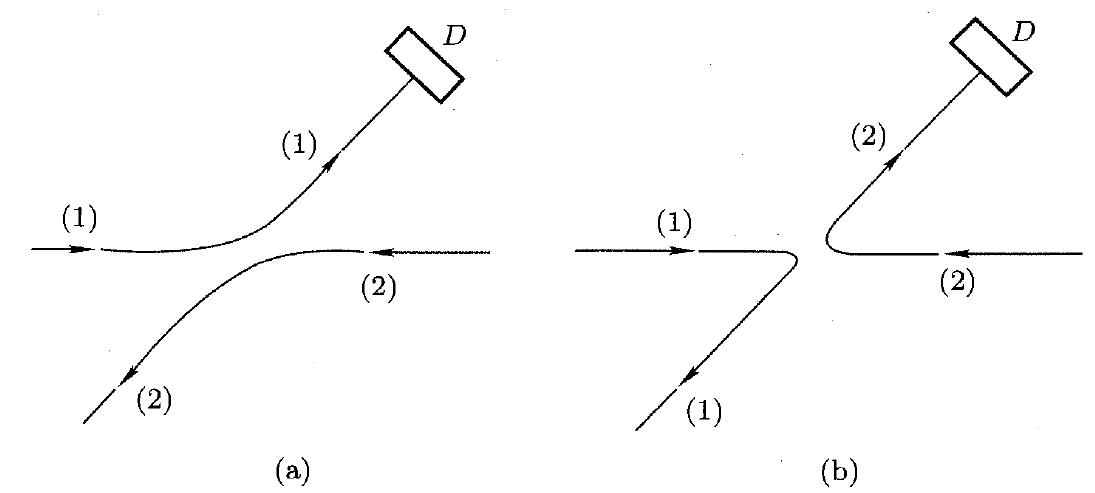
\includegraphics[width=0.6\textwidth]{figure/identicalparticles.png}
    \caption{两条可能的路径,探测器并不能分辨这两条路径对应的态}
    \label{fig:identicalparticles}
\end{figure}

上面的例子在初态的时候波包是分开的,因此初态是可以被唯一确定的,下面一个例子表明了初态也有可能不能被唯一确定,我们称这种类似的现象为交换简并。

考虑两个自旋为$\frac{1}{2}$的全同粒子,单粒子对应的自旋空间设为$\mathscr{E}_1,\mathscr{E}_2$,自旋空间上定义的自旋算符为$\hat{S_1},\hat{S_2}$。于是我们可以令$\hat{S_{1z}},\hat{S_{2z}}$的本征值为$\frac{\varepsilon_1}{2},\frac{\varepsilon_2}{2}$($\varepsilon_1,\varepsilon_2=\pm 1$)对应的共同本征态为$|\varepsilon_1,\varepsilon_2\rangle$。可以发现这个共同本征态集中存在两个态对应一个物理状态的情况,也即:
\begin{equation}
    |+,-\rangle,|-,+\rangle
\end{equation}

也就是说,该物理状态对应的右矢可以取这两个正交态张成的二维空间中的任意一个态:
\begin{equation}\label{equ11:A}
    |\psi\rangle=\alpha|+,-\rangle+\beta|-,+\rangle
\end{equation}

在上述背景下,量子力学假设应用于其上会产生问题。比如在初态为式\eqref{equ11:A}的情况下,求解为两个自旋在x轴方向本征值都为$+\frac{1}{2}\hbar$的概率,可以知道,末态应该为对应$|+\rangle_1$和$|+\rangle_2$的直积:
\begin{align}
    \begin{split}
        |\psi'\rangle=&\frac{1}{\sqrt{2}}(|\varepsilon_1=+\rangle+|\varepsilon_1\rangle)\otimes \frac{1}{\sqrt{2}}(|\varepsilon_2=+\rangle+|\varepsilon_2=-\rangle) \\
        =&\frac{1}{2}(|+,+\rangle+|+,-\rangle,|-,+\rangle,|-,-\rangle)
    \end{split}
\end{align}

于是根据量子力学假设,对应的概率为:
\begin{equation}
    P=|\langle \psi|\psi'\rangle|^2=|\frac{1}{2}(\alpha+\beta)|^2
\end{equation}

可以看到基于量子力学假设得到的概率依赖于系数$\alpha,\beta$,也即概率不确定,这是违背量子力学假设的。因此我们必须指出\eqref{equ11:A}式究竟用哪一个态而不能在二维空间中任意取,也即消除“交换简并”。

最后我们借由三全同粒子体系为例子扩展到一般N个全同粒子体系,表明全同粒子体系都会遇到交换简并的问题。对于三全同粒子体系,我们如果孤立的看待每个粒子,则每个粒子都对应一个态空间和对应的联络算符,则体系的态空间可以表示为:
\begin{equation}
    \mathscr{E}=\mathscr{E}_1\otimes\mathscr{E}_2\otimes\mathscr{E}_3
\end{equation}

设粒子(1)对应的联络算符为$\hat{B(1)}$,并且假设$\hat{B(1)}$构成$\mathscr{E}_1$的CSCO;由于三个粒子是全同粒子,因此粒子(2),(3)对应的联络算符应该为$\hat{B(2)},\hat{B(3)}$,并且本征值的谱都是相同的$\{b_i\}$,利用三个单粒子空间的基,通过张量积的形式,我们可以构造$\mathscr{E}$上的正交归一基:
\begin{equation}
    \{|1:b_i,2:b_j,3:b_p\rangle,i,j,k=1,2,\dots\}
\end{equation}

全同粒子不能让我们测量到$\mathscr{B}(1),\mathscr{B}(2),\mathscr{B}(3)$,因为粒子的编号毫无意义,但是我们可以测量物理量$\mathscr{B}$。假定测量的结果为$b_p,b_q,b_k$,则以下态是无法分辨的:
\begin{align}
    \begin{split}
        |1:b_p,2:b_q,3:b_k\rangle,&|1:b_p,2:b_k,3:b_q\rangle,|1:b_q,2:b_p,3:b_k\rangle,\\
        |1:b_q,2:b_k,3:b_p\rangle,&|1:b_k,2:b_p,3:b_q\rangle,|1:b_k,2:b_q,3:b_p\rangle
    \end{split}
\end{align}

上述交换简并导致$\hat{B}$无法分辨态空间上的这些态。我们可以很容易的推广到N个全同粒子的情况,由此我们可以看到,对于全同粒子的完全测量(与CSCO有关)不能在体系中确定唯一的态。
\section{置换算符的基本性质}
    根据上面的讨论,我们可以发现交换简并的出现实际上与标号的顺序有关,同一组数的序数排列共同构成了交换简并态。根据这个性质,我们引入了置换算符的概念来处理同一组数的序数排列问题,通过引入置换算符,我们可以简化全同粒子假设带来的推论与计算的有用工具,下面我们介绍一下基本的符号与性质。
    \subsection{两个粒子的体系}
    我们首先考虑简单情况,即自旋相同的两粒子体系。由于全同粒子带来交换简并的干扰,因此我们在本章中都人为的认为粒子都是可以分辨的,记作粒子(1)与粒子(2)。同时我们假设单粒子的自旋空间是同构的,因此对于自旋算符,$\mathscr{E}_1,\mathscr{E}_2$可以采用同一组基。于是态空间上的一组基可以表示为两个单粒子自旋空间的自旋算符对应态的张量积:
    \begin{equation}
        \mathscr{E}:|1:u_i;2:u_j\rangle
    \end{equation}
    
    定义的张量积的顺序是无关的:
    \begin{equation}
        |1:u_i;2:u_j\rangle=|2:u_i;1:u_j\rangle
    \end{equation}
    此时我们定义置换算符,它对基矢量的作用为:
    \begin{equation}
        \hat{P_{21}}|1:u_i;2:u_j\rangle=|2:u_i;1:u_j\rangle=|1:u_j;2:u_i\rangle
    \end{equation}
    
    上式说明置换算符的作用是交换两个粒子的自旋状态。置换算符具有一些良好的性质。首先,根据置换算符的定义,我们可以知道置换算符一定满足幂等性:
    \begin{equation}
        \hat{P_{21}}^2=\hat{P_{21}}
    \end{equation}
    
    同时我们也可以证明置换算符是一个厄米算符,即:
    \begin{equation}
        \hat{P_{21}}^\dagger=\hat{P_{21}}
    \end{equation}
\begin{proof}
    要想证明置换算符的厄米性,我们只需要证明算符在一组基下对应的矩阵元关系满足:
    \begin{equation}
        P_{mn}=P_{nm}^*
    \end{equation}
    
    我们考虑$\{|1:u_i;2:u_j\rangle\}$上的矩阵元:
    \begin{align}
        \begin{split}
            P_{mn}=&\langle 1:u_{i'};2:u_{j'}|\hat{P_{21}}|1:u_i;2:u_j\rangle\\
            =&\langle 1:u_{i'};2:u_{j'}||1:u_j;2:u_i\rangle\\
            =& \delta_{i'j}\delta_{ij'}\\
            P_{nm}^*=&(\langle 1:u_i;2:u_j|\hat{P_{21}}|1:u_{i'};2:u_{j'})^*\\
            =&(1:u_i;2:u_j|1:u_{j'};2:u_{i'})^*\\
            =&\delta_{i'j}\delta_{ij'}
        \end{split}
    \end{align}
    
    可以发现$\hat{P_{21}}$在$\{|1:u_i;2:u_j\rangle\}$上的矩阵元$P_{mn},P_{nm}^*$相等
\end{proof}

    根据置换算符的厄米性和幂等性,我们可以知道置换算符是幺正的:
    \begin{equation}
       \hat{P_{21}}\hat{P_{21}}^\dagger =(\hat{P_{21}})^2=\hat{I}
    \end{equation}
    
    由于置换算符是厄米的,因此它的本征值是实数,设$|\psi\rangle$是$\hat{P_{21}}$的本征态,由于幂等性,因此$\hat{P_{21}}^2$的本征值为1:
    \begin{equation}
        \hat{P_{21}}^2|\psi\rangle=|\psi\rangle
    \end{equation}
    
    所以$\hat{P_{21}}$的本征值为+1或-1,其中我们称本征值为+1的本征态是对称态,记作$|\psi_S\rangle$;本征值为-1的本征态为反对称态,记作$|\psi_A\rangle$:
    \begin{align}
        \begin{split}
            \hat{P_{21}}|\psi_S\rangle=&|\psi_S\rangle\\
             \hat{P_{21}}|\psi_A\rangle=&-|\psi_A\rangle
        \end{split}
    \end{align}
    
    在得到了对称态与反对称态的概念以后,接下来我们考虑如何通过构造投影算符构造对称态与反对称态,我们引入两个与$\hat{P_{12}}$有关的算符\footnote{在后面的内容中我们将会知道为什么算符会呈现这样的形式}:
    \begin{align}
        \begin{split}
            \hat{S}=&\frac{1}{2}(1+\hat{P_{21}})\\
            \hat{A}=&\frac{1}{2}(1-\hat{P_{21}})
        \end{split}
    \end{align}
    
    可以验证,$\hat{S},\hat{A}$同样满足幂等性,厄米性和幺正性。同时我们根据定义可以知道$\hat{S}$和$\hat{A}$是对易和互补的,即:
    \begin{align}
        \hat{S}\hat{A}=\hat{A}\hat{S}=&0\\
        \hat{S}+\hat{A}=&\hat{I}
    \end{align}
        
    上式说明$\hat{S}$和$\hat{A}$对态空间上任意态的投影作用可以构造两个互补的正交子空间\footnote{因为对于态空间上任意的态$|\psi\rangle$,都满足:
    \begin{align*}
        \hat{S}(\hat{A}|\psi\rangle)=&0\\
        \hat{A}(\hat{S}|\psi\rangle)=&0
    \end{align*}
    }
    \subsection{N个粒子的体系}
    我们可以将两个粒子的置换算符拓展到N个粒子的体系,为了简单的说明拓展定义的变动之处,我们首先考虑N=3的情况。
    
    假设三个同构的可分辨粒子的自旋空间,同时使用同一组基底$\{u_i\}$进行描述,则整个态空间上的基可以表示为:
    \begin{equation}
        \mathscr{E}:\{|1:u_i;2:u_j;3:u_k\rangle\}
    \end{equation}
    
    其对应的6个置换算符为:
    \begin{align}
        \begin{split}
            \hat{P_{123}},& \hat{P_{132}}, \hat{P_{213}}\\
             \hat{P_{231}},& \hat{P_{312}}, \hat{P_{321}}
        \end{split}
    \end{align}
    
    置换算符作用到对应的基矢量的表达式为:
    \begin{equation}
        \hat{P_{npq}}|1:u_i;2:u_j;3:u_k\rangle=|n:u_i;p:u_j;q:u_k\rangle
    \end{equation}
    
    其中$n,p,q$是1,2,3的一种序数排列。通过观察$N=3$的6个置换算符,我们可以简单验证,这6个置换算符的集合构成一个群。
    \begin{proof}
        简单验证一下六个置换算符的集合构成一个置换群。
        
        首先可以通过下表验证封闭性:
        \begin{table}[h]
            \centering
           \begin{tabular}{ |c||c|c|c|c|c|c|  }
         \hline
         \quad&$\hat{P_{123}}$& $\hat{P_{132}}$&$\hat{P_{213}}$&$\hat{P_{231}}$&$\hat{P_{312}}$&$ \hat{P_{321}}$\\
         \hline\hline
          $\hat{P_{123}}$&$\hat{P_{123}}$&$ \hat{P_{132}}$&$\hat{P_{213}}$&$\hat{P_{231}}$&$\hat{P_{312}}$&$ \hat{P_{321}}$\\
         \hline
         $\hat{P_{132}}$&$\hat{P_{132}}$&$\hat{P_{123}}$&$\hat{P_{312}}$&$\hat{P_{213}}$&$\hat{P_{321}}$&$\hat{P_{231}}$\\
         \hline
         $\hat{P_{213}}$&$\hat{P_{213}}$&$\hat{P_{231}}$&$\hat{P_{123}}$&$\hat{P_{321}}$&$\hat{P_{132}}$&$\hat{P_{312}}$\\
         \hline
         $\hat{P_{231}}$&$\hat{P_{231}}$&$\hat{P_{213}}$&$\hat{P_{321}}$&$\hat{P_{123}}$&$\hat{P_{132}}$&$\hat{P_{312}}$\\
         \hline
         $\hat{P_{312}}$&$\hat{P_{312}}$&$\hat{P_{321}}$&$\hat{P_{132}}$&$\hat{P_{231}}$&$\hat{P_{123}}$&$\hat{P_{213}}$\\
         \hline
         $\hat{P_{321}}$&$\hat{P_{321}}$&$\hat{P_{312}}$&$\hat{P_{231}}$&$\hat{P_{132}}$&$\hat{P_{213}}$&$\hat{P_{123}}$\\
         \hline
        \end{tabular}
            \caption{三个全同粒子的置换算符乘法表}
            \label{permutationgroup}
        \end{table}
        
        由上表我们可以发现,对于三全同粒子体系,任意两个置换算符$\hat{P_\alpha}$,$\hat{P_{\beta}}$,我们总能找到一个置换算符$\hat{P_\gamma}$,满足$\hat{P_\alpha}\hat{P_{\beta}}=\hat{P_{\gamma}}$。此外同样根据上表我们可以验证乘法的分配律和结合律,这个集合的单位元是$\hat{P_{123}}$,每个置换算符的逆元是它本身。
    \end{proof}
    
    类似的,我们可以拓展到N个粒子的体系,对应定义N!个置换算符,并且这N!个置换算符构成一个置换群。与两全同粒子体系类似,我们在这里引入两个重要的算符$\hat{S},\hat{A}$,其定义为:
    \begin{align}
        \begin{split}
            \hat{S}=&\frac{1}{N!}\sum_\alpha \hat{P_\alpha}\\
            \hat{A}=&\frac{1}{N!}\sum_\alpha \varepsilon_\alpha\hat{P_\alpha}
        \end{split}
    \end{align}
    
    其中当$\alpha$为偶排列时,$\varepsilon=+1$;当$\alpha$为奇排列时,$\varepsilon=-1$。可以发现在两粒子的体系中,我们定义的算符是上式的一个特例;并且在这个特例中,我们知道这两个算符是两个正交子空间的投影算符,并且定义了对称态与反对称态,类似的,在N个全同粒子体系中我们也能定义:
    \begin{align}
        \begin{split}
            \hat{P_\alpha}|\psi_S\rangle=&|\psi_S\rangle\\
            \hat{P_\alpha}|\psi_A\rangle=&\varepsilon_\alpha|\psi_A\rangle
        \end{split}
    \end{align}
    
    我们称$|\psi_S\rangle$为完全对称态,称$|\psi_A\rangle$为完全反对称态。
    \begin{remark}
    在上面的叙述中我并没有说$\hat{S},\hat{A}$将态拆成两个正交子空间,态只有对称态与放对称态,因为当$N>2$的时候,由于奇排列的出现导致这条性质不成立。比如对于$N=3$的全同粒子体系:
    \begin{equation}
        \hat{S}+\hat{A}=2(\hat{P_{123}}+\hat{P_{231}}+\hat{P_{312}})\ne \hat{I}
    \end{equation}
    \end{remark}
    
    此外,在两全同粒子体系中还证明了$\hat{S},\hat{A}$是并且满足幂等性,厄米性,对易性。那么N个全同粒子的体系定义的算符是否满足这些性质呢?首先由于$\hat{P_\alpha}$都是厄米的,因此$\hat{S},\hat{A}$也是厄米的,即:
    \begin{align}
        \begin{split}
            \hat{S}^\dagger=&\hat{S}\\
            \hat{A}^\dagger=&\hat{A}
        \end{split}
    \end{align}
    
    其次,对于某个置换算符$\hat{P_{\alpha_0}}$,我们可以有以下关系:
    \begin{align}\label{equ11:B}
        \begin{split}
            \hat{P_{\alpha_0}}\hat{S}=&\hat{S}\\
            \hat{P_{\alpha_0}}\hat{A}=&\varepsilon_{\alpha_0}\hat{A}
        \end{split}
    \end{align}
    
    由于置换算符是封闭的,因此对于给定的两个置换算符$\hat{P_{\alpha_0}},\hat{P_\alpha}$,一定存在一个置换算符$\hat{P_\beta}$满足$\hat{P_{\alpha_0}}\hat{P_\alpha}=\hat{P_\beta}$。同时,对于$\hat{A}$来说,常数$\varepsilon$也满足对应关系:$\varepsilon_\beta=\varepsilon_{\alpha_0}\varepsilon_\alpha$根据这个性质,考虑某个置换算符$\hat{P_{\alpha_0}}$对$\hat{S}$的作用,则有:
    \begin{equation}
        \hat{P_{\alpha_0}}\hat{S}=\frac{1}{N!}\sum_\alpha \hat{P_{\alpha_0}}\hat{P_\alpha}=\frac{1}{N!}\sum_\beta \hat{P_\beta}=\hat{S}
    \end{equation}
    
    同理,用同样的思路可以得到$\hat{P_{\alpha_0}}$对$\hat{S}$的作用:
    \begin{equation}
        \hat{P_{\alpha_0}}\hat{A}=\frac{1}{N!}\sum_\alpha \varepsilon_\alpha\hat{P_{\alpha_0}}\hat{P_\alpha}=\frac{1}{N!}\varepsilon_{\alpha_0}\sum_\beta \hat{P_\beta}=\varepsilon_{\alpha_0}\hat{A}
    \end{equation}
    
    如果$\hat{P_{\alpha_0}}$右乘在$\hat{S},\hat{A}$旁,证明是类似的。
    
    根据\eqref{equ11:B},我们可以推得:
    \begin{align}
        \begin{split}
            \hat{S}^2=&\hat{S}\\
            \hat{A}^2=&\hat{A}
        \end{split}
    \end{align}
    
    同时,$\hat{A}$和$\hat{S}$之间是对易的,即:
    \begin{equation}
        \hat{A}\hat{S}=\hat{S}\hat{A}=0
    \end{equation}
    
    这是因为:
    \begin{align}
        \begin{split}
            \hat{S}^2=&\frac{1}{N!}\sum_\alpha\hat{P_\alpha}\hat{S}=\frac{1}{N!}\sum_\alpha\hat{S}=\hat{S}\\
            \hat{A}^2=&\frac{1}{N!}\sum_\alpha\varepsilon_\alpha\hat{P_\alpha}\hat{A}=\frac{1}{N!}\sum_\alpha\hat{A}=\hat{A}
        \end{split}
    \end{align}
    
    上两式的最后一个等号是由于$\alpha$共有N!种排列,并且$\hat{S},\hat{A}$与$\alpha$无关。对易关系也是类似的证明:
    \begin{equation}
        \hat{A}\hat{S}=\frac{1}{N!}\sum_\alpha\varepsilon_\alpha\hat{P_\alpha}\hat{S}=\frac{1}{N!}\sum_\alpha\varepsilon_\alpha\hat{S}=\frac{\hat{S}}{N!}\sum_\alpha \varepsilon_\alpha=0
    \end{equation}
    
    其中,上式最后一个等号是因为对于数排列$\alpha$,奇排列个数等于偶排列个数。由此,我们证明了$\hat{S},\hat{A}$是态空间$\mathscr{E}$的两个正交子空间$\mathscr{E}_S,\mathscr{E}_A$的投影算符,即:
    \begin{align}
        \hat{S}\hat{P_\alpha}=\hat{P_\alpha}\hat{S}|\psi\rangle=&\hat{S}|\psi\rangle\\
        \hat{A}\hat{P_\alpha}=\hat{P_\alpha}\hat{A}|\psi\rangle=&\varepsilon_\alpha\hat{A}|\psi\rangle
    \end{align}
    在N个全同粒子体系中构造的两个投影算符$\hat{S},\hat{A}$和它们导出的一系列性质在后续说明的过程中起到非常重要的作用。
\section{对称化假设}
    \subsection{对称化假设的引入与交换简并的消除}
    为了消除交换简并带来的困难,我们引入对称化假设:
    \begin{definition}{对称化假设}{symmetry}
        对于全同粒子体系,如果交换粒子,对应的物理右矢只能是完全对称的或是完全反对称的。如果物理右矢是完全对称的,对应的粒子称为玻色子;如果物理右矢是完全反对称的,对应的粒子称为费米子。
    \end{definition}
    
    上述定义表明全同粒子的态空间不再是$\mathscr{E}$,而是其子空间,是$\mathscr{E}_S$还是$\mathscr{E}_A$取决于粒子的性质。我们知道引入对称化假设的目的在于消除交换简并,那么对称化假设是如何消除交换简并的呢?
    
    首先回顾一下前面的内容,假设$|u\rangle$是N个全同粒子体系的一个完全确定的状态,根据上面内容的讨论,我们可以知道$\hat{P_\alpha}|u\rangle$和$|u\rangle$可以描述同一个物理状态。换句话说一个物理状态位于由$\hat{P_\alpha}|u\rangle$的全体构成的态空间$\mathscr{E}$的子空间$\mathscr{E}_u$。如果$dim\mathscr{E}_u>1$,则会出现交换简并现象。而对称化假设告诉我们,描述物理状态的右矢一定位于$\mathscr{E}_S$中(如果粒子是玻色子)或者$\mathscr{E}_A$中(如果粒子是费米子)。那么问题就转换为了我们需要证明:$\mathscr{E}_u$只含有$\mathscr{E}_S/\mathscr{E}_A$的一个右矢。
    
    根据上一节的推导,我们知道投影算符满足关系:$\hat{S}=\hat{S}\hat{P_\alpha}$,$\hat{A}=\varepsilon_\alpha\hat{A}\hat{P_\alpha}$。于是对于态空间$\mathscr{E}$上任意的一个完全确定的态$|u\rangle$,我们知道:
    \begin{align}
        \begin{split}
            \hat{S}=&\hat{S}(\hat{P_\alpha}|u\rangle)\\
            \hat{A}=&\varepsilon_\alpha\hat{A}(\hat{P_\alpha}|u\rangle)
        \end{split}
    \end{align}
    
    上式说明$|u\rangle$和所有$\hat{P_\alpha}|u\rangle$在$\mathscr{E}_S$或$\mathscr{E}_A$中的投影都是共线的。也就是说,我们只需要求出$\hat{S}|u\rangle$或$\hat{A}|u\rangle$就能作为物理状态唯一的右矢了(以下简称为物理右矢)。
    \subsection{物理右矢的构造}\label{subsection:physicalket}
    根据上面的讨论,我们知道物理右矢的构造分为3步:
    \begin{itemize}
        \item 对所有粒子编号(编号仅仅为了书写的方便,而不是表明粒子之间是可分辨的),通过单粒子空间上的基构造态空间上的与某个物理状态对应的态$|u\rangle$;
        \item 根据粒子是玻色子还是费米子,将$\hat{S}$算符或者$\hat{A}$算符作用到$|u\rangle$上;
        \item 对物理右矢进行归一化;
    \end{itemize}
    
    为了生动的理解构造的过程,我们举一个简单的例子。考虑两全同粒子体系,我们令粒子(1)处于已经归一化的单粒子态$|\phi\rangle$上,令粒子(2)处于另一个已经归一化的单粒子态$|\chi\rangle$上,那么:
    \begin{equation}
        |u\rangle=|1:\phi;2:\chi\rangle
    \end{equation}
    
    如果粒子是玻色子的话,则物理右矢可以表示为:
    \begin{equation}
        \hat{S}|u\rangle=\frac{1}{2!}(\hat{P_{12}}+\hat{P_{21}})|u\rangle=\frac{1}{2}(|1:\phi;2:\chi\rangle+|1:\chi;2:\phi\rangle)
    \end{equation}
    
    如果粒子是费米子的话,则物理右矢可以表示为:
    \begin{equation}
        \hat{A}|u\rangle=\frac{1}{2!}(\varepsilon_{12}\hat{P_{12}}+\varepsilon_{21}\hat{P_{21}})|u\rangle=\frac{1}{2}(|1:\phi;2:\chi\rangle-|1:\chi;2:\phi\rangle)
    \end{equation}
    
    最后考虑归一化,如果$|\phi\rangle$和$|\chi\rangle$是正交的,那么归一化因子很容易求出:只要将上述两式前的系数换成$\frac{1}{\sqrt{2}}$即可。
    \begin{remark}
    考虑一种特殊情况:$|\phi\rangle=|\chi\rangle$,此时观察费米子的物理右矢,你会发现$\hat{A}|u\rangle=\frac{1}{2}(|1:\phi;2:\phi\rangle-|1:\phi;2:\phi\rangle)=0$,也就是说当费米子处于两个相同的单粒子态的时候,$\mathscr{E}_A$中没有一个非平凡的右矢可以代表这个物理状态,这种情况下是违背对称化假设的,我们称其为Pauli不相容原理。这个原理在后续的讨论中有重要意义。
    \end{remark}
    
    对于N=3的情况,我们可以类似的令$|u\rangle$的形式为:
    \begin{equation}
        |u\rangle=|1:\phi;2:\chi;3:\varphi\rangle
    \end{equation}
    
    则对于玻色子的情况,物理右矢可以表示为:
    \begin{align}
         \begin{split}
             \hat{S}|u\rangle=&\frac{1}{3!}(|1:\phi;2:\chi;3:\varphi\rangle+|1:\phi;3:\chi;2:\varphi\rangle+|2:\phi;1:\chi;3:\varphi\rangle+\\
             &|2:\phi;3:\chi;1:\varphi\rangle+|3:\phi;1:\chi;2:\varphi\rangle+|3:\phi;2:\chi;1:\varphi\rangle)
         \end{split}
    \end{align}
       
     对于费米子来说,物理右矢可以表示为:
     \begin{align}
         \begin{split}
             \hat{S}|u\rangle=&\frac{1}{3!}(|1:\phi;2:\chi;3:\varphi\rangle-|1:\phi;3:\chi;2:\varphi\rangle-|2:\phi;1:\chi;3:\varphi\rangle+\\
             &|2:\phi;3:\chi;1:\varphi\rangle+|3:\phi;1:\chi;2:\varphi\rangle-|3:\phi;2:\chi;1:\varphi\rangle)
         \end{split}
    \end{align}
    
    可以发现,上式的定义正好符合行列式的定义\footnote{因为行列式其中一种定义正好也是与数的奇排列偶排列有关},于是我们可以写成一个更紧凑的行列式形式,即Slater行列式:
    \begin{equation}
        \hat{A}|u\rangle=\frac{1}{3!}\begin{vmatrix}
            |1:\phi\rangle&|1:\chi\rangle&|1:\varphi\rangle\\
            |2:\phi\rangle&|2:\chi\rangle&|2:\varphi\rangle\\
            |3:\phi\rangle&|3:\chi\rangle&|3:\varphi\rangle
        \end{vmatrix}
    \end{equation}
    
    如果有两个单粒子态相同,则有行列式中有两列相同,因此行列式等于0,因此Pauli不相容原理在N=3也是成立的。如果$|\phi\rangle,|\chi\rangle,|\varphi\rangle$是正交的,那么归一化只要将$\frac{1}{3!}$换成$\frac{1}{\sqrt{3!}}$即可。
    
    类似的结论可以推广到N个全同粒子的体系,即我们可以用单粒子态去构成玻色子的物理右矢;用Slater行列式构成费米子的物理右矢。同时由于行列式的特殊性导致Pauli不相容原理仍然成立,这一点造成了费米子与玻色子的区别。
    \begin{remark}
        Pauli不相容原理会导致玻色子和费米子的性质有很大的不同。其中,玻色子在低温出现的一种现象被称为玻色-爱因斯坦凝聚,其本质就在于在低温的时候,玻色子能够“一窝蜂”地挤到最低能级中去,而费米子却要受到Pauli不相容原理的限制。一个著名的例子就是He-3具有的超流动性,就是因为He-3是玻色子。
    \end{remark}
    \subsection{构成物理右矢基的构造}
    本节我们讨论N个全同粒子的体系如何构造物理右矢的一组基:首先我们选择单粒子态空间上的一组基$\{|u_i\rangle\}$构成态空间$\mathscr{E}$上的一组基:
    \begin{equation}
        \mathscr{E}:\{|1:u_i;2:u_j;\dots;N:u_p\rangle\}
    \end{equation}
    
    根据对称化假设,物理右矢一定位于$\mathscr{E}_S$或$\mathscr{E}_A$上,因此我们考虑$\hat{S}/\hat{A}$作用于基$\{|1:u_i;2:u_j;\dots;N:u_p\rangle\}$上,得到张成空间$\mathscr{E}_S$或$\mathscr{E}_A$的矢量集合。
    \begin{remark}
    比如我们考虑一个在$\mathscr{E}_S$空间上的态$|\varphi\rangle$,由于$\mathscr{E}_S$一定是$\mathscr{E}$的一个子空间,则$|\varphi\rangle$一定可以可以用$\mathscr{E}$上的基$\{|1:u_i;2:u_j;\dots;N:u_p\rangle\}$线性表示:
    \begin{equation}
        |\varphi\rangle=\sum_{i,j,\dots,p}a_{i,j,\dots,p}|1:u_i;2:u_j;\dots;N:u_p\rangle
    \end{equation}
    
    根据定义:$|\varphi\rangle\in\mathscr{E}_S$,因此一定有关系:
    \begin{equation}
        \hat{S}|\varphi\rangle=|\varphi\rangle
    \end{equation}
    
    联立两式可得:
    \begin{equation}
         |\varphi\rangle=\sum_{i,j,\dots,p}a_{i,j,\dots,p}(\hat{S}|1:u_i;2:u_j;\dots;N:u_p\rangle)
    \end{equation}
    
    可以发现:$\hat{S}|1:u_i;2:u_j;\dots;N:u_p\rangle$就是张成空间$\mathscr{E}_S$的矢量集合。
    \end{remark}
    
    但是这样运算存在一个问题,即$\hat{S}|1:u_i;2:u_j;\dots;N:u_p\rangle$并不是线性无关的!(比如$\hat{S}\hat{P_\alpha}|1:u_i;2:u_j;\dots;N:u_p\rangle$就与$\hat{S}|1:u_i;2:u_j;\dots;N:u_p\rangle$对应同一个物理状态)。为了解决这个问题,我们引入占有数的概念\footnote{这个概念的提出非常自然,我的理解是,全同粒子的问题本质上就是相同小球的排列组合问题,我们需要时刻考虑到单纯排列带来的重复}:
    \begin{definition}{占有数}{occupynumber}
        对于态$|1,u_i;2,u_j;\dots;N,u_p\rangle$,单粒子态$|u_k\rangle$的占有数$n_k$等于$|u_k\rangle$在$\{|u_i\rangle,|u_j\rangle,\dots,|u_p\rangle\}$中出现的次数。
    \end{definition}
    
    如果对于各单粒子态的占有数分别是相等的,则态可以通过置换算符的作用进行转换,并且这些转换的态对应同一个物理右矢,记作$|n_1,n_2,\dots,n_k\rangle$,称为粒子数表象。这个概念将会在后续的二次量子化中继续深入讨论。

    \section{与其它量子力学假设的相容性}
    本节主要想论证在对称化假设的框架下,其它量子力学假设也能与之相容,其中主要包含两点:
    \begin{itemize}
        \item 只使用$\mathscr{E}_S$/$\mathscr{E}_A$中的物理右矢去描述测量过程;
        \item $|\psi(t)\rangle$经过演化后不会超出$\mathscr{E}_S$/$\mathscr{E}_A$
    \end{itemize}
    
    换句话说,我们希望其它量子力学假设在$\mathscr{E}_S$/$\mathscr{E}_A$空间上成立。
    
        \subsection{与测量与算符假设的相容}
        我们假设测量前的态是$|\psi(t)\rangle$;显然,根据对称化假设,$|\psi(t)\rangle$一定属于$\mathscr{E}_S$或$\mathscr{E}_A$。经过测量物理量$\mathscr{A}$以后,态变为了物理右矢$|u\rangle$,其中$|u\rangle$可以通过\ref{subsection:physicalket}节中的方法构造。如此,初态和末态都在$\mathscr{E}_S$/$\mathscr{E}_A$中,那么所有量子力学的结果就取决于标量积$\langle \psi|u\rangle$和矩阵元$\langle\psi|\hat{A}|u\rangle$了,我们先考虑标量积$\langle \psi|u\rangle$。
        
                \begin{remark}
        全同粒子的测量与非全同粒子的测量有什么不同呢?我们在第二章讲述概率幅与测量的关系的时候曾经见过一个连续测量的例子:如果我们对中间态进行测量,那么我们必须对概率幅进行求和,这样就产生了干涉效应;而如果我们确定了一个具体的中间态的话,那么我们只能根据经典粒子的情况对概率分别进行求和,干涉效应消失。在这里是一样的想法,由于全同粒子的特点,其根据对称性与反对称性构造的物理右矢$|u\rangle$相当于中间态,当对全同粒子进行测量的时候,我们应该对概率幅相加,此时会产生由交换导致的干涉效应;而当粒子非全同的时候,相当于我们确认了全同粒子全排列中的一种,此时测量,干涉效应消失。
        
        为了方便理解,这里举一个两个全同粒子测量的例子。假设两个全同粒子在测量前处于两个相互正交的单粒子态$|\chi\rangle,|\varphi\rangle$,则根据对称化假设,对应的物理右矢应该满足:
        \begin{equation}
            |\varphi,\chi\rangle=\frac{1}{\sqrt{2}}(1+\varepsilon\hat{P_{21}})|1:\varphi;2:\chi\rangle
        \end{equation}
        
        其中:
        \begin{equation}
            \varepsilon=\left\{
            \begin{array}{cc}
                +1 & \text{粒子是玻色子} \\
                -1 & \text{粒子是费米子}
            \end{array}
            \right.
        \end{equation}
        
        当体系处于$|\varphi,\chi\rangle$态时,对整个体系进行物理量$\mathscr{B}$的测量,对应的测量算符满足下列本征方程:
        \begin{equation}
            \hat{B}|u_i\rangle=b_i|u_i\rangle
        \end{equation}
        
        我们要考虑的问题是求得特定结果($b_m,b_n$)的概率。此时,末态根据对称化假设可以得到:
        \begin{equation}
            |u_m,u_n\rangle=\frac{1}{\sqrt{2}}(1+\varepsilon\hat{P_{21}})|1:u_m;2:u_n\rangle
        \end{equation}
        
        因此,概率幅可以表示为:
        \begin{equation}
            \langle u_m,u_n|\varphi,\chi\rangle=\frac{1}{2}\langle 1:u_m;2:u_n|(1+\varepsilon\hat{P_{21}}^\dagger)(1+\varepsilon\hat{P_{21}})|1:\varphi;2:\chi\rangle
        \end{equation}
        
        由于:
        \begin{align}
            \begin{split}
                \frac{1}{2}(1+\varepsilon\hat{P_{21}}^\dagger)(1+\varepsilon\hat{P_{21}})=&\frac{1}{2}\big(1+\varepsilon(\hat{P_{21}}^\dagger+\hat{P_{21}})+\varepsilon^2\hat{P_{21}}^2\big)\\
                =&\frac{1}{2}\big(1+\varepsilon(\hat{P_{21}}^\dagger+\hat{P_{21}})+1\big)\\
                =&1+\varepsilon \hat{P_{21}}
            \end{split}
        \end{align}
        
        代入概率幅公式可以得到:
        \begin{align}
            \begin{split}
                 \langle u_m,u_n|\varphi,\chi\rangle=&\frac{1}{2}\langle 1:u_m;2:u_n|(1+\varepsilon\hat{P_{21}})|1:\varphi;2:\chi\rangle\\
                 =&\langle 1:u_m;2:u_n|1:\varphi;2:\chi\rangle+\varepsilon\langle 1:u_m;2,u_n|1:\chi;2:\varphi\rangle\\
                 =&\langle 1:u_m|1:\varphi\rangle\langle 2:u_n|2:\chi\rangle+\varepsilon\langle 1:u_m|1:\chi\rangle\langle2:u_n|2:\varphi\rangle\\
                 =& \langle u_m|\varphi\rangle\langle u_n|\chi\rangle+\varepsilon\langle u_m|\chi\rangle\langle u_n|\varphi\rangle
            \end{split}
        \end{align}
        
        上式可以理解为初态到末态的两条路径的干涉(形象的表示如图\eqref{fig:identical_interfere}),于是目标的概率为:
        \begin{equation}
            P(b_m;b_n)=| \langle u_m,u_n|\varphi,\chi\rangle|^2
        \end{equation}
        
        \begin{figure}[H]
            \centering
            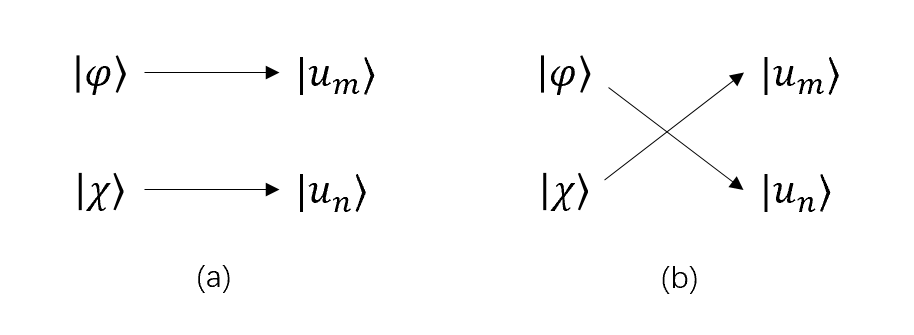
\includegraphics[width=0.9\textwidth]{figure/identical_interfere.png}
            \caption{两全同粒子体系的直接项(a)与交换项(b)的示意图}
            \label{fig:identical_interfere}
        \end{figure}
        
        通常我们称概率幅公式的第一项为直接项,第二项为交换项。当体系是全同粒子态的时候,直接项的概率幅与交换项的概率幅会产生干涉。其中,玻色子以"+"干涉,费米子以"-"干涉。
        \end{remark}
        
        显然,根据上面的描述,标量积可以通过$\mathscr{E}_S$/$\mathscr{E}_A$中的两个矢量进行描述,不同的地方在于:如果$\hat{A}$是一个完全的测量(就是构成$\mathscr{E}_S/\mathscr{E}_A$上的ESCO,比如测量全体粒子的位移$r$和自旋分量$S_x$),则$|u\rangle$一定是唯一的;如果$\hat{A}$是一个不完全的测量(就是不构成$\mathscr{E}_S/\mathscr{E}_A$上的ESCO),则物理右矢$|u\rangle$有若干个(并且是相互正交的)。
        \begin{remark}
        比如我们考虑态空间$\mathscr{E}$上的一个态$|1:u_i;2:u_j;\dots;N:u_p\rangle$,完全测量就是完全确定了全同粒子状态的集合$\{|u_i\rangle,|u_j\rangle,\dots,|u_p\rangle\}$,则根据对称化假设的讨论,符合条件的物理右矢是唯一的;不完全测量指的就是不能完全获得全同粒子的状态(比如仅仅测量了1个粒子的位移和自旋或是只测了所有粒子的自旋),这样我们知道满足条件的物理状态不止一个,自然物理右矢$|u\rangle$也不止一个。但是由于本征态的性质,不同本征态对应的右矢是正交的,因此不同的$|u\rangle$也是正交的。
        \end{remark}
       
        接下来我们讨论算符假设的相容性。什么算符能够表示全同粒子系的物理状态呢?我们抓住全同粒子系本身的特点,即交换粒子并不会改变体系的物理状态,也就是说,如果对于物理状态$|u\rangle$,用$\hat{G}$测量$|u\rangle$以后,交换粒子并不会改变测量后的物理状态$\hat{G}|\psi\rangle$。由于置换算符有关系:
        \begin{equation}
            \hat{P_\alpha}|\psi\rangle=\varepsilon_\alpha|\psi\rangle
        \end{equation}
        
        那么上述论述可以表示为:
        \begin{equation}
            \hat{P_\alpha}\hat{G}|\psi\rangle=\hat{G}\hat{P_\alpha}|\psi\rangle=\varepsilon_\alpha\hat{G}|\psi\rangle
        \end{equation}
        
        由此我们可以知道,描述物理状态的算符$\hat{G}$与置换算符之间满足关系:
        \begin{equation}\label{equ11:communitive}
            [\hat{G},\hat{P_\alpha}]=0
        \end{equation}
        
        上式一方面表明$\hat{G}$在$\mathscr{E}_S/\mathscr{E}_A$下不变;同时也表明算符$\hat{G}$对所有粒子具有交换对称性。
        
        \subsection{与Schrodinger方程的相容}
        本节考虑状态演化的相容性,考虑在$\mathscr{E}_S/\mathscr{E}_A$下的一个含时物理右矢$|\psi(t)\rangle$,我们知道Schrodinger方程:
        \begin{equation}
            i\hbar\frac{d|\psi(t)\rangle}{dt}=\hat{H}|\psi(t)\rangle
        \end{equation}
        
        由于$d|\psi(t)\rangle=|\psi(t+dt)\rangle-|\psi(t)\rangle$,因此上式可以化简为:
        \begin{equation}
            |\psi(t+dt)\rangle=\big(1+\frac{dt}{i\hbar}\hat{H}\big)|\psi(t)\rangle
        \end{equation}
        
        我们将$\hat{P_\alpha}$作用于上式,结合\eqref{equ11:communitive}式,我们可以得到:
        \begin{equation}
            \hat{P_\alpha}|\psi(t+dt)\rangle=\hat{P_\alpha}\big(1+\frac{dt}{i\hbar}\hat{H}\big)|\psi(t)\rangle=\big(1+\frac{dt}{i\hbar}\hat{H}\big)(\hat{P_\alpha}|\psi(t)\rangle)
        \end{equation}
        
        该式表明$\hat{P_\alpha}|\psi(t)\rangle$经过演化得到$\hat{P_\alpha}|\psi(t+dt)\rangle$。进一步,如果$|\psi(t)\rangle$是$\hat{P_\alpha}$的本征态,那么$|\psi(t+dt)\rangle$也是$\hat{P_\alpha}$的本征态并且本征值相同,因此粒子是费米子还是玻色子并不随着状态的演化而改变。换句话说Schrodinger方程并不会使$|\psi(t)\rangle$的演化超出$\mathscr{E}_S/\mathscr{E}_A$。

\part{量子化学基础}

\chapter{多电子原子}
    \begin{introduction}
    \item 基本概念
\end{introduction}

\section{基本概念}
    \subsection{原子单位制}
        在量子化学计算中,由于计算机的数值模拟只具有有限的精度,因此方程的系数往往会很大的影响到结果的准确性,为了最大限度地除去这类干扰,我们常常使用原子单位制来简化式子的表达。相比于一般的量子化学书对原子单位制的说明,我希望用稍微严谨一点的表述说明原子单位制的选取\footnote{本节内容主要参考了小时百科以及wiki有关Hartree atomic units的说明}。
        
        原子单位制的目的就是将方程去量纲化。首先考虑一个相对简单的粒子来引出大致的思路。考虑一维的含时Schrodinger方程:
        \begin{equation}
            -\frac{\hbar^2}{2m}\frac{\partial^2\Psi}{\partial x^2}+V\Psi=i\hbar \frac{\partial \Psi}{\partial t}
        \end{equation}
        
        我们将上式所有的物理量转换为无量纲的量,即:$x=x_a\beta_x,m=m_a\beta_m,V=V_a\beta_V,\psi=\psi_a\beta_{\psi},t=t_a\beta_t$,其中诸如$x_a,m_a$之类的量都是没有量纲的。代入上式并化简即可以得到:
        \begin{equation}
            -\Big(\frac{\hbar^2}{\beta_m\beta_x^2\beta_E}\Big)\frac{1}{2m_a}\frac{\partial^2\psi_a}{\partial x_a^2}+V_a\psi_a=i\Big(\frac{\hbar}{\beta_t\beta_E}\Big)\frac{\partial\psi_a}{\partial t_a}
        \end{equation}
        
        唯一可能含有量纲的数就是$\frac{\hbar^2}{\beta_m\beta_x^2\beta_V},\frac{\hbar}{\beta_t\beta_V}$。为了得到不含有量纲的方程,我们人为地令这两个量为1,即:
        \begin{align}\label{equ12:restrictA}
            \begin{split}
                \frac{\hbar^2}{\beta_m\beta_x^2\beta_E}=&1\\
                \frac{\hbar}{\beta_t\beta_E}=&1
            \end{split}
        \end{align}
        
        同时考虑波函数地归一,我们可以得到另一个无量纲组合量:
        \begin{align}\label{equ12:restrictB}
                1=\int |\Psi|^2dx=(\beta_{\psi})^2\beta_x\int \psi^2_adx_a=(\beta_{\psi})^2\beta_x
        \end{align}
        
        特别的,对于N维波函数,我们可以很容易地推广得到:
        \begin{equation}
            (\beta_{\psi})^2\beta_x^N=1
        \end{equation}
        
        由\ref{equ12:restrictA},\ref{equ12:restrictB}式,我们可以知道上述量的自由度为2(比如说知道了$\beta_x,\beta_m$,我们就可以推出其它所有的量)。一般来说,我们令$\beta_m$为电子的质量,$\beta_x$为Bohr半径,于是我们可以得到其它量的取值:
       \begin{align}
           \begin{split}
               \beta_E=&\frac{\hbar^2}{m_ea_0^2}\\
               \beta_t=&\frac{m_ea_0^2}{\hbar}
           \end{split}
       \end{align}
       
       我们称$\beta_E$的单位为Hartree。简单来说,我们可以认为原子单位制就是将$\hbar,a_0.e,m_e$四个量变为1,上述四个量分别表示原子单位制下的运动,长度,电荷和质量量度。基于上面的“定义”,我们就可以将具有M个核子和N个电子的波函数的Hamiltonian写成如下简单的形式:
       \begin{equation}
           \hat{H}=-\sum_{A=1}^M\frac{1}{2M_A}\nabla^2_A-\sum_{i=1}^N\frac{1}{2}\nabla_i^2+\sum_{A=1}^{M}\sum_{B>A}^M\frac{Z_AZ_B}{R_{AB}}+\sum_{i=1}^{N}\sum_{j>i}^N\frac{1}{r_{ij}}-\sum_{i=1}^N\sum_{A=1}^M\frac{Z_A}{r_{iA}}
       \end{equation}
       
       式中,$A,B$是核的标号,$i,j$是电子的标号,$Z_A,Z_B$为核子的标号。上述五项分别表示核的动能,电子的动能,核之间的相互作用,电子之间的相互作用,核与电子之间的相互作用。
    \subsection{B-O近似}
        由上节的讨论,虽然我们已经写出了一般具有M个核子,N个电子的体系Hamiltonian的表达式,由此我们可以写出多电子体系对应的定态方程:
        \begin{equation}\label{equ12:multiele_stationaryA}
            \hat{H}\psi(q_i,Q_j)=E\psi(q_i,Q_j)
        \end{equation}
        
        其中$q_i$是电子的广义坐标;$Q_j$是核的广义坐标。虽然定态方程的形式看上去非常简单,但是实际上这个体系是一个多体问题,不能精确求解,因此我们需要发展各种合理的近似手段去化简方程。这其中最基本最简单但是较为精确的假设就是Born-Oppenheimer近似。
        \subsubsection{定核假设}
        B-O近似的本质在于分离核与电子的运动,这个想法的出发点在于核子与质子的质量差别很大(即$m_n>>m_e$),因此可以知道核子的运动是比电子慢很多的。于是对于原子核的每一次微小运动,我们可以认为电子总是能够迅速地跟上核的运动并迅速适应新的势场(即电子对核运动的响应是瞬时的\footnote{简单来说,相对于电子的运动,我们可以忽略核的运动})。于是我们自然可以假设原子核处在空间任意一个相对位置时,分子的电子状态和原子核一直固定在空间某一点对应的分子的电子状态相等。这也表明电子总是在固定的核势场中运动,从而对于\ref{equ12:multiele_stationaryA}式的定态方程的Hamiltonian,如果我们只考虑电子的运动,此时我们可以忽略核的动能项,得到电子运动的定态方程:
        \begin{equation}
            (\hat{H_{el}})\psi_{el}=E^{el}\psi_{el}
        \end{equation}
        
        其中:
        \begin{align}\label{equ12:multiele_stationaryB}
                \hat{H_{el}}=-\sum_{i=1}^N\frac{1}{2}\nabla_i^2+\sum_{i=1}^{N}\sum_{j>i}^N\frac{1}{r_{ij}}-\sum_{i=1}^N\sum_{A=1}^M\frac{Z_A}{r_{iA}}+\sum_{A=1}^{M}\sum_{B>A}^M\frac{Z_AZ_B}{R_{AB}}
        \end{align}
        
        其中$E^{el}$是包含了核子之间相互作用的电子能量,对于一般我们的讨论来说,$R_{AB}$是一个不随电子坐标改变的常数,但是势能的大小却与核的构型(configuration)有关,因此我们可以明确\ref{equ12:multiele_stationaryB}式的函数形式:
        \begin{align}
            \begin{split}
                \psi_{el}=&\psi_{el}(q_i,Q_j)\\
                E^{el}=&E^{el}(Q_j)
            \end{split}
        \end{align}
        
        其中$q_\alpha$是参数(parameter),$q_i$是变量(variable)。
        \subsubsection{绝热近似}
        假设电子的Schrodinger方程已经被完全求解,下面我们讨论核运动。根据上面的讨论,由于电子对核运动的响应是瞬时的,因此当核进行移动时,我们可以忽略电子运动的影响。换而言之,核的运动是核的构型的函数,我们可以将电子看作连接核的弹簧,因此核运动产生的势场应该包含了核的相互作用以及电子对核产生的势场,即$E^{el}(Q_j)$;同时考虑其动能,因此我们可以写出核运动的定态方程:
        \begin{align}
            \begin{split}
                \hat{H_N}\psi_N(Q_j)=E\psi_N(Q_j)
            \end{split}
        \end{align}
        
        其中\footnote{该式的$j$是一个常数,不是一个变化的值,代表核受到电子的某种势场作用}:
        \begin{equation}
            \hat{H_N}=-\sum_{A=1}^M\frac{1}{2M_A}\nabla^2_A+E^{el}(Q_j)
        \end{equation}
        
        $E$和\ref{equ12:multiele_stationaryA}式中的$E$一样,代表体系的总能量,是一个常数。上述论述统称为绝热近似(adiabatic approximation)。Born和Fork对绝热近似的定义是\footnote{wiki上的原文为:A physical system remains in its instantaneous eigenstate if a given perturbation is acting on it slowly enough and if there is a gap between the eigenvalue and the rest of the Hamiltonian's spectrum}:一个物理系统保持在它的瞬时本征态,如果给定的扰动作用在它上的速度足够慢,并且在本征值和哈密顿谱的其余部分之间有一个间隙。可以看到,这里的绝热与热力学的绝热\footnote{热力学中的绝热指体系不与环境发生热量和物质的交换}不同,反倒和准静态过程的定义类似,我的理解为\footnote{这里的理解基于wiki的词条,词条的原文为:Gradually changing conditions allow the system to adapt its configuration, hence the probability density is modified by the process. If the system starts in an eigenstate of the initial Hamiltonian, it will end in the corresponding eigenstate of the final Hamiltonian.}:体系运动的每一步由于弛豫\footnote{所谓弛豫涉及到两个时间:"内部"时间$T_i$,代表体系自身运动;"外部"运动$T_e$,代表环境参数变化的时间。弛豫就是这两个时间的博弈,显然,绝热近似要求$T_e>>T_i$}较大(有点像平衡态的感觉),因此当核从$Q_j$移动到$Q_{j'}$时,我们可以认为电子没有受到核运动的扰动发生电子的跃迁,此时势能函数永远都是$Q_j$的函数,如此,系统的每一个状态都是构型的函数。
        
        \begin{remark}
        这里有两个例子帮助您更好的理解绝热近似的思想\footnote{这两个绝好的例子可以在wiki和Griffiths的CH7中找到}:第一个例子是无阻尼单摆在一个箱子里摆动。试想,如果我拿着箱子猛烈地移动它,那么单摆一定会混乱的移动;而如果我缓慢的移动这个箱子,那么单摆仍然会相对于箱子做振幅一样的往复摆动。
        \begin{figure}[H]
            \centering
            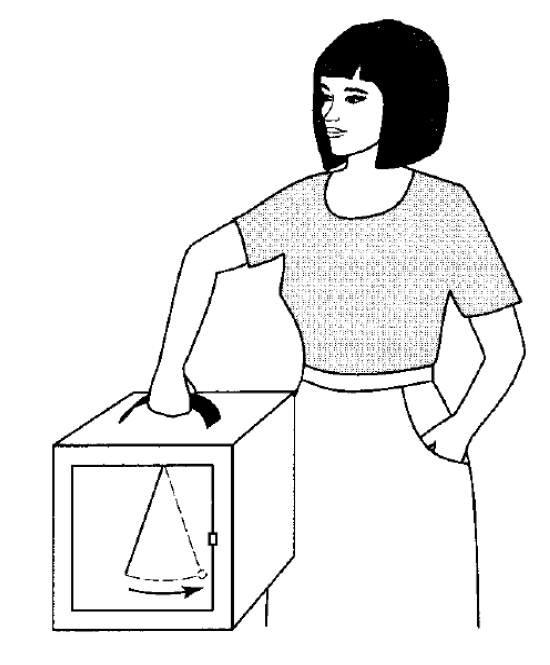
\includegraphics[width=0.5\textwidth]{figure/adiabaticprocess.png}
            \caption{如果箱子移动得非常缓慢,里面的摆将在与原来平面平行的平面振动,振幅保持不变}
            \label{fig:adiabaticprocess}
        \end{figure}
        
        根据这个例子启发,我们可以将核看作我们提的箱子,而将电子看作往复运动的单摆。由于核的运动相比电子来说很慢,因此核无论处于什么位置,我们都能得到电子的能量。换句话说,电子的能量$E^{el}$是以核的坐标位参数的(即$E^{el}(Q_1,Q_2,\dots,Q_m)$),我们称此时的电子能量构成势能面(potential energy surface)
        
        这个例子是对绝热运动的形象理解。分析这类问题,一般来说先把外部参数设为常量,在求解到最后的时候再允许外部参数随时间变化。一个经典的例子\footnote{这个方法在定核近似中其实已经分析过了}是氢原子离子的求解,我们先假设原子核质心距离为R,然后求解电子的运动。如果我们求解出了能量,再令R是能量的函数,从而可以得到平衡位置和原子核振动的频率。这种先固定原子核位置(可以理解为变量参数化),再求解电子运动,最后利用电子运动的信息得到核运动的信息就是B-O近似的核心思想。
        \end{remark}
        
        我们下面较为严格的证明绝热近似。
        
        
        定核近似与绝热近似合在一起称为B-O近似。可以发现,在该近似下,多电子体系的Hamiltonian被分解为了核运动算符$\hat{H_N}$与电子运动算符$\hat{H_{el}}$的直和。因此方程的解可以写成核运动波函数与电子运动波函数的直接乘积:
        \begin{equation}
            \psi(q_i,q_\alpha)=\psi_N(q_\alpha)\psi_{el}(q_i,q_\alpha)
        \end{equation}
        
        在量子化学的学习中,我们往往更为重视电子的运动,因为它决定着物质的化学性质。

\appendix
\part{附录} 
\chapter{线性代数基础}
    \begin{introduction}
    \item 线性空间基础
    \item 线性映射基础
    \item 线性算子基本理论
    \item 具有度量的线性空间
\end{introduction}
本附录是理解笔记的基础,讲述线性代数最基本也是最核心的概念---线性空间和线性映射,所有的内容都是基于这两点进行展开。本章的难度比简单介绍概念要深,同时为了逻辑的顺畅,增加了一些超出量子力学需要的内容。限于自己的能力,本附录对于矩阵与行列式的引入没有做很好的说明。
\section{线性空间}
    \subsection{线性空间的概念}
    我们的第一个目标就是搞懂线性空间的结构是怎么样的。为了方便理解,我们可以通过思考$Euclid$空间来进行类比。在$Euclid$空间中,我们除了可以将其看作许多点以外;我们还可以通过在空间内定义一个零点,考虑所有以零点出发的向量的集合来构成这个空间。
    
    在这里,我们的思路是后者。此时我们的目标就从“线性空间是什么?”变成了“向量是什么?”了。在数学中,“是什么”的问题往往是通过它具备什么性质入手解决的。因此在这里我们就需要考虑向量具有的性质是什么。根据高中所学,我们知道向量具有加法与数量乘法两种运算,并且运算满足加法交换律、结合律、乘法分配律、结合律,同时具有零元、负元。那么我们可以认为线性空间就是满足以上性质的集合。
    
    但是在具体给出线性空间的严格证明之前还存在一个问题:什么是运算?我们从小时候就懂得如何使用数运算,因此以整数域上的加法运算为例子,考虑$2+3=5$。事实上,从映射的角度上来看就是构成了二元数组到整数域上的映射:$(2,3)\rightarrow5$,于是我们可以得到集合上运算的概念:
    \begin{definition}{运算}{calculate}
       我们定义$ S\times M=\{ (a,b),a\in S,b\in M \}$为$S$和$M$的笛卡尔积。如此,我们就称$S\times S\rightarrow S$称为$S$的一个代数运算
    \end{definition}
    
    由此我们可以定义线性空间的概念:
    \begin{definition}{线性空间}{vectorspace}
       设$V$是一个非空集合,$F$是一个数域,我们在$V$上规定了两种运算:加法与数量乘法,其中加法是$V\times V \rightarrow V$的映射,定义为:$(\alpha,\beta)\rightarrow \alpha+\beta $;数量乘法是$K\times V \rightarrow V$的映射,定义为:$(k,\alpha)\rightarrow k\alpha$,并且满足8条运算法则,则称$V$是一个线性空间
       \begin{enumerate}
           \item{(加法交换律)} $\alpha+\beta$=$\beta+\alpha$
           \item{(加法结合律)} $(\alpha+\beta)+\gamma=\alpha+(\beta+\gamma)$
           \item{(零元)} $V$中存在一个元素,称为零元,满足$0+a=a+0$
           \item{(负元)} $\forall a\in V$,都存在一个元素$\beta$,使得$\alpha+\beta =\beta +\alpha =0$,则称$\beta $为逆元,记作$\beta =-\alpha $
           \item{(数量乘法的单位元)} $1\alpha =\alpha 1=1$
           \item{(结合律)}$(kl)\alpha=k(l\alpha )$
           \item{(分配律1)}$(k+l)\alpha=k\alpha+l\alpha,
           \forall k,l\in F $
           \item{(分配律2)}$k(\alpha+\beta)=k\alpha+k\beta , \forall k,l\in F $
       \end{enumerate}
    \end{definition}
    
    可以看到,所谓线性空间,不过是一个定义了一些代数结构的集合而已,于是我们就可以将集合论中的一些概念迁移到其上。其中,最关键的一个概念就是集合的子集。在实际运用中,我们常常希望集合的子集能够保持原来集合的结构。由此我们引入了子空间的概念:
    \begin{definition}{子空间}{subspace}
       设$U$是线性空间$V$的一个子集,如果$V$的8条运算性质对于$U$中任意元素$\delta $都成立,则称$U$是线性空间的一个子空间。
    \end{definition}
    \subsection{张成、线性无关、基、维数}
        \subsubsection{线性组合,张成,线性表出}
            根据线性空间中加法与数量乘法两种运算,我们可以得到线性组合的定义:
            \begin{definition}{线性组合}{linearcombination}
               $a_1,a_2,\ldots,a_m$是线性空间$V$的一组向量组,设$c_1,c_2,\ldots ,c_m\in F$,则称$c_1a_1+c_2a_2+\ldots +c_ma_m$为$a_1,a_2,\ldots a_m$的一个线性组合,$c_1,c_2,\ldots ,c_m$称为系数
            \end{definition}
            对比子空间的概念,我们知道 $a_1,a_2,\ldots,a_m$这组向量组的所有线性组合的集合构成一个线性空间,并且容易证明,这个线性空间一定是$V$的一个子空间,于是我们引入张成空间的概念:
            \begin{definition}{张成空间与线性表出}{span}
            我们称线性空间$V$的子空间$\{c_1a_1+c_2a_2+\ldots +c_ma_m, c_1,c_2,\ldots ,c_m\in F\}$为向量组$a_1,a_2,\ldots,a_m$所张成的空间,记作:$span(a_1,a_2,\ldots,a_m)$。
            
            反之,如果$V$中的向量$\beta$,存在一组数域$F$的数$k_1,k_2,\ldots ,k_m$,使得$\beta=k_1a_1+k_2a_2+\ldots +k_ma_m$,则称$\beta$能被向量组$a_1,a_2,\ldots,a_m$线性表出
            \end{definition}
            
            易得张成空间与线性表出是等价的:
            
            \begin{corollary}{张成空间与线性表出的等价性}{spanlinear}
                \begin{equation*}
                    \beta \in span(a_1,a_2,\ldots,a_m)\Longleftrightarrow \beta \textrm{能被向量组}a_1,a_2,\ldots,a_m \textrm{线性表出}
                \end{equation*}
            \end{corollary}
            
        \subsubsection{线性无关,基,维数}
        对于$\textrm{能被向量组}a_1,a_2,\ldots,a_m \textrm{线性表出}$的向量$\beta$来说,一个很重要的问题在于其表示是否是唯一的。假设有两组数组$\{c_1,c_2,\ldots ,c_m \},\{d_1,d_2,\ldots ,d_m \}$,使得:
            \begin{align}
                \begin{split}
                    \beta =&c_1a_1+c_2a_2+\ldots +c_ma_m\\
                    \beta =&d_1a_1+d_2a_2+\ldots +d_ma_m\\
                \end{split}
            \end{align}
            
        两式相减,可得:
            \begin{equation}
                0=(c_1-d_1)a_1+(c_2-d_2)a_2+\ldots +(c_m-d_m)a_m
            \end{equation}
        
        上式可以认为是向量组$a_1,a_2,\ldots,a_m $对零元的表达。考虑到线性空间中零元一般是唯一的,因此我们希望上式对于任何符合要求的$c_i,d_i$恒成立(也就是说向量组$a_1,a_2,\ldots,a_m $是一个性质”好“的向量组),于是只有:
            \begin{equation}
               c_1=d_1;c_2=d_2,\ldots;c_m=d_m
            \end{equation}
            
        因此,由零元的表达唯一,我们就可以推出任何线性空间内的向量在”好“向量组$a_1,a_2,\ldots,a_m $下的表达都应该是唯一的。这种想法与集合中元素必须要满足唯一表达的原因类似,否则我们无法对集合中的元素建立映射。由”好“向量组,我们引出线性无关的概念:
        \begin{definition}{线性相关与线性无关}{linearindependent}
        如果$c_1a_1+c_2a_2+\ldots +c_ma_m$成立当且仅当$c_1=c_2=\cdots=c_m=0$,则称向量组$a_1,a_2,\ldots,a_m$线性无关;反之,如果存在一组不全为0的数组$d_1,d_2,\ldots ,d_m$,使得$d_1a_1+d_2a_2+\ldots +d_ma_m=0$,则称向量组$a_1,a_2,\ldots,a_m$线性相关
        \end{definition}
        
        我们现在已经知道线性无关的向量组的表达是唯一的,这是描述线性空间的基础。如果我们需要描述线性空间V话,我们最朴素的想法在于选取尽可能少的元素来得到线性空间V的全部信息(这个想法对应在集合论中叫做集合的代表)。因此我们希望选取一组线性无关的向量组的同时这一组向量组还能张成V。前面一条保证了V的每一个向量都能被唯一表示(唯一性);后面一条确保V中每一个向量都能被这一组向量组表示(遍历性)。由此我们定义了基的概念:
        \begin{definition}{基}{basis}
        如果线性空间V上的一个向量组线性无关的同时又能张成线性空间V,则称这个向量组是线性空间V上的一组基
        \end{definition}
        
        现在我们做进一步考虑。如果V中所有的向量都可以被向量组$a_1,a_2,\cdots ,a_m$线性表出,但是$a_1,a_2,\cdots,a_m$是线性相关的。根据前面的讨论,当我们想用$a_1,a_2,\cdots,a_m$描述线性空间V中的向量时,它的表示不是唯一的。但是按照基的想法,我们希望寻找$a_1,a_2,\cdots,a_m$的一个部分组$a_{i_1},a_{i_2},\cdots,a_{i_m} (i_m\leq m)$,这个部分组是线性无关的,但是这个部分组同样能够张成V\footnote{换句话说,部分组组$a_{i_1},a_{i_2},\cdots,a_{i_m}$是V的一组基}。可以想象,这个部分组一定是向量组的临界情况:即只要往部分组里加任意一个向量进去,加入新向量后的新部分组一定线性相关。于是我们得到极大线性无关组的概念:
        \begin{definition}{极大线性无关组}{maxlinearinde}
            如果线性空间V向量组$a_1,a_2,\cdots,a_m$的一个部分组$a_{i_1},a_{i_2},\cdots,a_{i_m}$满足:
            \begin{itemize}
                \item 这个部分组线性无关
                \item 从这个向量组的其它向量中任意选一个加入这个部分组,新的部分组是线性相关的
            \end{itemize}
            
            则称这个部分组为极大线性无关组。
        \end{definition}
        对比定义\ref{def:maxlinearinde}和定义\ref{def:basis}我们可以很直观的发现极大线性无关组就是空间V的一组基,但是很自然的产生了另一个问题:线性空间中的基并不是唯一的,那么不同基之间有什么共性吗?我们考虑空间V的两组基$B_1,B_2$,如果我们认为$B_1$是极大线性无关组,$B_2$张成空间V,那么两者的向量组的长度一定满足$B_1\leq B_2$;反之,如果$B_1$张成空间V,$B_2$是极大线性无关组,那么$B_2\leq B_1$,于是一定有$B_1=B_2$。即线性空间V中任意一组基的长度都是相等的,由此我们定义维数:\footnote{由于当向量组的长度为无穷时不能按照上述方法进行比较,因此本笔记中不考虑无穷维数的情况}
        \begin{definition}{维数}{dimention}
            有限维空间V的任意基的长度称为V的维数,记作dimV
        \end{definition}
        
        如此,我们就得到了描述线性空间的第一种途径:选取V上的一组基,由此V上的每一个向量都可以被这组基的线性组合唯一表示。同时空间的维数保证了基选取的任意性和等价性。
    \subsection{子空间的交、和与直和}
    本节,我们想探究如何从子空间出发研究线性代数的结构。从直觉上来讲,如果关系是从部分到整体的话,往往在最后会出现将不同部分组合起来看的情况。举一个例子,当我们利用分离变量法求解微分方程时,求解出分离变量后的特征值方程的通解以后,为了得到原来微分方程的通解,我们的方法就是将所有特征值方程的通解进行叠加。我们知道,线性空间V的本质就是一个集合,在高中的时候我们学习了不同集合之间的运算关系,即集合的交与并。集合的交和并可以缩小或者扩大集合,这正是我们希望得到的。那么更进一步,我们自然希望线性空间V的子空间的交和并仍然具有一个好的结构,即它仍然是V的子空间。这样保证了相同的运算规律为我们处理问题带来了方便。
    
    首先我们看一下两个线性子空间的交是不是子空间。设V的两个不相同的子空间$V_1,V_2$,任取$V_1\bigcap V_2$的两个元素$\alpha,\beta$,下面我们注意对照线性空间的性质验证。首先,$0\in V_1\bigcup V_2。$ 由于$\alpha,\beta\in V_1\bigcap V_2$,那么$\alpha,\beta\in V_1\textrm{且}\alpha,\beta\in V_2$。由于子空间的加法对$V_1,V_2$封闭,因此$\alpha+\beta\in V_1\textrm{且}\alpha,\beta\in V_2$。同理,我们可以验证数乘运算同样对$V_1\bigcap V_2$封闭;于是两个子空间的交是一个子空间。进一步,我们可以利用数学归纳法推广这个定理,即:
    \begin{theorem}{子空间的交是子空间}{cupissubspace}
    设$I$是一个指标集,对于每一个$i\in I$,$V_i$是$V$的子空间,令:
    \begin{equation}
        \bigcap_{i=1}V_i=\{\alpha\in V|\alpha\in V_i,i\in I\}
    \end{equation}
    
    则$\bigcap_{i=1}V_i$是一个子空间。
    \end{theorem}
    
    但是,子空间的并一般不是一个子空间。比如在一个平面中选取任意两条直线$l_1,l_2$,分别取$l_1,l_2$上的两个向量,记作$\gamma_1,\gamma_2$,显然$\gamma_1+\gamma_2\notin l_1\cup l_2$。我们的想法是构造一个扩大集合的工具,于是我们可以定义一个运算使得运算后的集合既包含子空间的并又是一个子空间。由上面的反例我们可以得到一点启示,因为任意两条直线的并只是两条直线,而如果我们要得到子空间的话,由于加法运算的存在,最小包含$l_1\cup l_2$的子空间应该是这两条直线上任意向量张成的平面。换句话说,我们的目标应该在定义中保证线性空间中加法运算的成立。于是我们定义子空间和的概念:\begin{definition}{两个子空间的和}{sumof2subspace}
        设线性空间$V$的两个不相同的子空间$V_1,V_2$,其中$\alpha_1\in V_1,\beta\in V_2$,于是我们构造下列集合:
        \begin{equation}
            V_1+V_2 :=\{\alpha+\beta|\alpha_1\in V_1,\beta\in V_2\}
        \end{equation}
        
        我们称$V_1+V_2$为子空间$V_1\textrm{与}V_2$的和。
    \end{definition}
    
    通过对比子空间的性质,我们可以简单得到$V_1+V_2$是$V$的一个子空间。我们同样可以利用数学归纳法推广到$n$个子空间的情况:
    \begin{theorem}{n个子空间的和}{sumofnsubspace}
    对于$V$的子空间$V_1,V_2,\dots,V_n$,下列集合:
    \begin{equation}
        \sum_{i=1}^n V_i=V_1+V_2+\dots+V_n:=\{\alpha_1+\alpha_2+\dots+\alpha_n|\alpha_1\in V_1,\alpha_2\in V_2,\dots,\alpha_n\in V_n\}
    \end{equation}
    则$\sum_{i=1}^n V_i$一定是$V$的一个子空间。
    \end{theorem}
    
    我们根据子空间的和从而将不同的子空间组合到了一起,但是子空间中的和中向量的表示不唯一。比如下图中的向量$\Vec{a}$,既可以表示为$\Vec{b_1}+\Vec{c_1}$,又可以表示为$\Vec{b_2}+\Vec{c_2}$
    %缺少一张图片
    
    于是我们自然想到:能不能对子空间的和这个概念加一些额外的限制条件使得向量能被唯一表示。观察下图的例子,如果直线$l$不在平面$\pi$内,那么我们可以发现,空间中任意一个向量$\Vec{b}$都可以唯一的表示为直线$l\textrm{上的某个向量}\Vec{a_1}$和平面$\pi\textrm{上的某个向量}\Vec{a_2}$的和。于是我们自然的引入了直和的概念:
    \begin{definition}{直和的直观定义}{directsum}
        如果$V$的子空间$V_1,V_2,\dots,V_n$的和$V_1+V_2+\dots+V_n$中的每一个元素都可以被唯一的表示,那么称和$V_1+V_2+\dots+V_n$为直和,记作$V_1\oplus V_2\oplus\dots\oplus V_n$
    \end{definition}

    事实上,唯一表示的概念出现在之前对线性代数线性无关的讨论中,我们可以知道线性无关概念的引入是基于线性空间中0元的表示是唯一而得来的,因此我们自然可以猜测以下有关0元与基的命题等价\footnote{这里为了证明的便利,我们写出2个子空间直和的定理,n个子空间直和的定理可以通过数学归纳法证明}:
    \begin{theorem}{两个子空间的直和的等价命题}{directsum}
        \begin{enumerate}
            \item $V_1+V_2$是直和
            \item $V_1+V_2$中0元表示方法唯一。即$\alpha_1+\alpha_2=0,\alpha_1\in V_1,\alpha_2\in V_2\Longleftrightarrow\alpha_1=\alpha_2=0$
            \item $V_1\cap V_2=\{0\}$
            \item $V_1$的一个基和$V_2$的一个基合起来是$V$的一个基
        \end{enumerate}
    \end{theorem}
    \begin{proof}
    $(1)\Rightarrow(2)$:由直和的定义可以立即得到;
    
    $(2)\Rightarrow(3)$:任取$\alpha\in V_1\cap V_2$,则有$\alpha\in V_1\textrm{并且}\alpha\in V_2$,由于$V_2$是$V$的子空间,于是$-\alpha\in V_2$,于是一定有关系:
    \begin{equation}
        \alpha +(-\alpha)=0 ,\alpha\in V_1;-\alpha\in V_2
    \end{equation}
    
    可以发现,上式满足命题(2),于是$\alpha=0$
    
    $(3)\Rightarrow(1)$:要想证明$V_1+V_2$是直和,也即证明$V_1+V_2$中所有元素能被唯一的表示。我们与线性无关的引入类似,采用反证法证明。假设$V_1+V_2$中任意一个元素$\alpha$有两种表示:
    \begin{align}
        \begin{split}
            \alpha=\alpha_1+\alpha_2,\alpha_1\in V_1,\alpha_2\in V_2\\
            \alpha=\beta_1+\beta_2,\beta_1\in V_1,\beta_2\in V_2
        \end{split}
    \end{align}
       
    于是$\alpha_1+\alpha_2=\beta_1+\beta_2$,即$\alpha_1-\beta_1=\alpha_2-\beta_2$。我们发现等号左边的元素属于$V_1$,等号右边的元素属于$V_2$,于是$\alpha_1-\beta_1\in V_1\cup V_2,\alpha_2-\beta_2\in V_1\cap V_2$。根据命题(3),我们知道$\alpha_1=\beta_1;\alpha_2=\beta_2$,即$\alpha$的表示方法唯一。
    
    $(2)\Rightarrow(4)$:假设$\eta_1,\eta_2,\dots,\eta_m$是$V_1$上的一组基,$\xi_1,\xi_2,\dots,\xi_n$是$V_2$上的一组基,我们需要证明$\eta_1,\eta_2,\dots,\eta_m,\xi_1,\xi_2,\dots,\xi_n$是$V$上的一组基,也即我们需要证明$\eta_1,\eta_2,\dots$,\\$\eta_m,\xi_1,\xi_2,\dots,\xi_n$线性无关并且张成空间$V$。
    
    首先证明线性无关,即证明下式成立:
    \begin{align}\label{equA:equ}
        \begin{split}
             a_1\eta_1+a_2\eta_2+\dots+a_m\eta_m+b_1\xi_1+b_2\xi_2+\dots+b_n\xi_n=0\\
             \Rightarrow a_1=a_2=\dots=b_1=b_2=\dots=b_n=0
        \end{split}
    \end{align}
       

    
    根据命题(2),我们有:
    \begin{align}
        \begin{split}
            a_1\eta_1+a_2\eta_2+\dots+a_m\eta_m=&0\Rightarrow a_1=a_2=\dots=a_m=0\\
            b_1\xi_1+b_2\xi_2+\dots+b_n\xi_n=&0 \Rightarrow b_1=b_2=\dots=b_n=0
        \end{split}
    \end{align}
    
    于是\ref{equA:equ}一定成立。下面讨论上述基能否张成空间$V$。由子空间和的定义,$V$中的任意一个元素$\alpha$一定可以表示为$V_1$上的一个元素$\alpha_1$和$V_2$上的一个元素$\alpha_2$之和。由于$\eta_1,\eta_2,\dots,\eta_m$是$V_1$上的一组基,因此$\alpha_1$一定可以被$\eta_1,\eta_2,\dots,\eta_m$线性表出;同理$\alpha_2$也一定可以被$\xi_1,\xi_2,\dots,\xi_n$线性表出。因此$\alpha$一定可以被$\eta_1,\eta_2,\dots,\eta_m,\xi_1,\xi_2,\dots,\xi_n$线性表出,证毕。
    
    $(4)\Rightarrow(2)$:我们最后需要考虑$V_1+V_2$上的零元的表示:$\alpha_1+\alpha_2=0.\alpha_1\in V_1,\alpha_2\in V_2$。于是对于下式:
    \begin{equation}
        0= (a_1\eta_1+a_2\eta_2+\dots+a_m\eta_m)+(b_1\xi_1+b_2\xi_2+\dots+b_n\xi_n)
    \end{equation}
    
    其中$\eta_1,\eta_2,\dots,\eta_m$是$V_1$上的一组基,$\xi_1,\xi_2,\dots,\xi_n$是$V_2$上的一组基,根据命题(4),我们知道$\eta_1,\eta_2,\dots,\eta_m,\xi_1,\xi_2,\dots,\xi_n$是$V$上的一组基,于是我们知道$a_1=a_2=\dots=b_1=b_2=\dots=b_n=0$,证毕。
    \end{proof}
    
    经过上述循环证明,我们就得到了上述命题之间相互等价。我们可以通过数学归纳法,将上述定理推广到n个子空间的直和的情况,此时最重要的结论就是直和与子空间上基的关系:
    \begin{theorem}{有限个子空间直和与子空间基的关系}{directsumandbasis}
        $V=V_1\oplus V_2 \oplus \dots \oplus V_n\Longleftrightarrow V_i$的一组基合起来是$V$的一组基
    \end{theorem}
    
    定理\ref{thm:directsumandbasis}告诉我们,我们可以通过将$V$分解为若干子空间的直和,并且研究子空间的性质再合并的方法研究线性空间。那么很自然的问题在于如何分解子空间呢?这个问题将在学习了集合的划分以及特征值以后得到解答。
    \subsection{集合的划分,等价关系和商空间}
   另一种处理线性空间的方法与集合的划分息息相关,换而言之我们希望对某一个整体进行合理的分类。首先通过一个例子引入相关的概念。生活中,我们往往会利用星期的概念对时间长河中的日子进行分类。如果使用数学语言描述这种现象,也就是将日子一一映射到整数集上。如果假设2021年1月10日对应数字0,那么其余日子就能分别对应其它数字了。我们定义星期几为这个日子对应数字被7除的余数,假设被7除余i的集合为$H_i,i=0,1,\dots,6$,那么整数集可以表示为:
   \begin{equation}
       \mathbb{Z}=H_0\cup H_1\cup \dots \cup H_6
   \end{equation}
   
   其中$H_i=\{7k+i|i=0,1,2,3,4,5,6;k\in\mathbb{Z}\}$。同时可以发现,当$i\ne j$时,$H_i\cap H_j=\emptyset$,由此我们可以抽象出集合的划分的概念:
   \begin{definition}{集合的划分}{setpartition}
       如果集合$S$是它的一些非空子集的并集,并且这些非空子集两两不相交,那么我们称这些非空子集组成的集合是集合$S$的一个划分。
   \end{definition}
   
   在星期的例子中,$\{H_0,H_1,H_2,H_3,H_4,H_5,H_6\}$是整数域$\mathbb{F}$的一个划分。
   
   在给出了集合的划分的概念后,下一个问题就是如何构造一种通用的划分集合的方法。我们从集合中的元素与划分后的非空子集间的关系入手。在星期的例子中,我们知道如果元素a,b同时处在同一个子集中当且仅当a与b被7除的余数相同,我们简称为a与b模7同余,记作$a\equiv b(mod7)$。同时我们称模7同余是$\mathbb{Z}$上的一个二元关系,在数学中,我们采用笛卡尔积来描述一个二元数组,于是元素a与b模7同余当且仅当:
   \begin{equation}
       (a,b)\in (H_0\times H_0)\cup (H_1\times H_1)\cup \dots \cup (H_6\times H_6)
   \end{equation}
   
   由于$(H_0\times H_0)\cup (H_1\times H_1)\cup \dots \cup (H_6\times H_6)$是$\mathbb{Z}\times\mathbb{Z}$的一个子集,我们记作$W$,于是元素a与b模7同余当且仅当$(a,b)\in W$,于是我们可以抽象出集合上的二元关系的定义:
   \begin{definition}{二元关系}{binaryrelation}
       对于非空集合$S$,我们称$S\times S$的一个非空子集$W$为集合$S$上的一个二元关系。如果对于$a,b\in S$,$(a,b)\in W$,则称$a,b$满足$W$关系,记作$a\sim b$;反之,如果$(a,b)\notin W$,则称$a,b$不满足$W$关系。
   \end{definition}
   
   进一步,观察模7同余这个二元关系,我们发现它满足以下三条性质:
   \begin{align}
       \begin{split}
           a\equiv& a(mod7)\\
          a\equiv b(mod7)&\Rightarrow b\equiv a\\
          a\equiv b(mod7),b\equiv c(mod7)&\Rightarrow a\equiv c(mod7)
       \end{split}
   \end{align}
   
   于是我们可以将其抽象得到等价关系的概念。
   \begin{definition}{等价关系}{equivrelation}
       定义$\sim$是$S$上的一个二元关系,如果$\sim$满足以下三条性质:\\
           (反身性) $a\sim a,\forall a\in S$\\
           (对称性) $a\sim b \Rightarrow b\sim a$\\
           (传递性) 若$a\sim b,b\sim c$,则$a\sim c$\\
       我们称$\sim \textrm{是}S$上的一个等价关系
   \end{definition}
   
   在星期的例子中,星期日是模7余0日子组成的集合,我们称为$\bar{0}$,其它集合也有类似的定义,于是我们可以抽象出等价类的概念:
   \begin{definition}{等价类与商集}{Equivalenceclass}
   设$\sim$是$S$上的一个等价关系,我们定义集合:
   \begin{equation}
       \bar{a}:=\{x\sim a,a\in S\}
   \end{equation}
   
   我们称$\bar{a}$为$a$的等价类,$a$称为$\bar{a}$的一个代表。同时我们称所有等价类组成的集合称为$S$的一个商集,记作$S/\sim$。
   \end{definition}
   
   如此定义后,我们发现在星期的例子中商集正好构成了$\mathbb{Z}$的一个划分,于是我们自然有以下定理:
   \begin{theorem}{等价类对集合划分}{partitionequivclass}
       设$\sim$是$S$上的一个等价关系,那么所有等价类组成的集合构成了$S$的一个划分。
   \end{theorem}
   
   \begin{proof}
   从定义出发,商集如果要成为一个划分,必须满足两个性质:商集中的元素之并等于$S$并且这些不相等的元素两两不相交。
   
   首先证明$\cup_{a\in S}\bar{a}=S$。首先根据定义,我们可以立即知道$\cup_{a\in S}\bar{a}\subseteq S$;同时,我们知道$\forall b\in S,b\in \bar{b}$,于是$b\in \cup_{a\in S}\bar{a}$,所以$S\subseteq \cup_{a\in S}\bar{a}$,因此$\cup_{a\in S}\bar{a}=S$。
   
   在证明不相等的商集中的元素两两不相交之前,我们需要首先了解以下相等的商集有什么性质,于是有以下引理:
   \end{proof}
   \begin{lemma}{相等的商集性质}{1}
   $\bar{a}=\bar{b}\Longleftrightarrow a\sim b$
   \end{lemma}
 \begin{proof}
   必要性:如果$\bar{a}=\bar{b}$,由于$a$是$\bar{a}$的一个代表,即$a\in \bar{a}$,于是$a\in \bar{b}$,根据等价类的定义,$a\sim b$;
   
   充分性:一般来说,常见的证明两个集合$A,B$相等就相当于分别证明$A$是$B$的子集同时$B$是$A$的子集。而$A$是$B$的子集相当于证明$\forall x\in A$,都有$x\in B$。
   
   在本证明中,由于$a\sim b,\forall c\in \bar{a}$,都有$c\sim a$,根据等价关系的传递性:$c\sim a,a\sim b$可以得到$c\sim b$,于是$c\in \bar{b}$。从而说明$\bar{a}\subseteq\bar{b}$;然后由于等价关系中的对称性,于是我们可以知道$b\sim a$,于是按照上面类似的步骤可知$\bar{b}\subseteq\bar{a}$
   
   随后我们可以证明不相等的商集中的元素两两不相交了:
 \end{proof}
   
   \begin{lemma}{不相等的商集元素两两不相交}{2}
  $\bar{a}\ne \bar{b}\Rightarrow\bar{a}\cap\bar{b}=\emptyset$
   \end{lemma}
   \begin{proof}
   这里我们使用反证法:假设$\bar{a}\cap\bar{b}=\emptyset$,那么一定存在一个元素$c\in \bar{a}
   \cap \bar{b}$,那么$c\in \bar{a},c\in \bar{b}$。利用等价类的定义我们可以得到$c\sim a,c\sim b$,于是$a\sim b$,根据引理\ref{lem:1},得到$\bar{a}=\bar{b}$,与题目条件矛盾,于是原命题成立。
   \end{proof}
   
   综上所述,在集合$S$上定义一个等价关系,那么等价关系导出的商集中的元素构成了$S$的一个划分,这是数学上对任意一个集合进行划分的普遍办法,在群论中也会用到类似的方法。
   
   那么迁移到线性代数的框架中,如果我们要划分一个线性空间$V$,我们需要在其上找到一个二元关系,如果它是$V$上的一个等价关系,那么这个关系对应的商集构成了$V$的一个划分。
   
   如何构造这个等价关系呢?我们观察几何空间的例子。对于三维空间,我们可以将一组平行平面构成三维几何空间的一组划分,因为所有平行平面加起来等于整个平面同时两两不相交。我们考虑这个例子的性质,我们首先找到对应的等价类,我们令此时过原点的平面为$\pi_0$,可以发现,所有等价类中只有$\pi_0$是三维空间的子空间,性质较好,因此我们尽量让定义的二元关系与$\pi_0$有关。我们选择平行于$\pi_0$的平面$\pi$上的两个点$b_1,b_2$,根据向量的减法,我们知道$\Vec{b_1},\Vec{b_2}$两个向量处于同一个平面当且仅当$\Vec{b_2}-\Vec{b_1}\in \pi_0$\footnote{这里很显然空间上的每个点总是可以和某个从原点引出到该点的向量一一对应的,因此我在描述的时候混用了两个概念}。于是我们可以抽象出这个二元关系:
   \begin{definition}{线性空间上的二元关系}{linearrelationonvecspace}
   令线性空间$V$的一个子空间为$W$,则可以定义二元关系如下:
   \begin{equation}
       \alpha\sim\beta\Longleftrightarrow \alpha-\beta \in W
   \end{equation}
   \end{definition}
   
   我们得到了线性空间上的一个二元关系,同时可以简单验证这个二元关系一定是等价关系:首先,由于$\alpha-\alpha=0\in W$,因此$\alpha\sim\alpha$,满足反身性;其次如果$\alpha\sim \beta$,根据定义有$\alpha-\beta\in W$根据线性空间的定义,该矢量一定有逆元$\beta-\alpha\in W$,因此$\beta\sim \alpha$,对称性满足;最后,由于$\alpha\sim\beta,\beta\sim \gamma$,因此一定有$\alpha-\beta+\beta-\gamma=\alpha-\gamma\in W$,即$\alpha\sim \gamma $,传递性满足。于是我们可以得到$\sim$是$V$上的一个等价关系。
   
   随后我们讨论这个等价关系对应等价类的形式:
   \begin{align}
       \begin{split}
           \bar{\alpha}=&\{\beta\in V|\beta\sim\alpha\}\\
           =&\{\beta\in V|\beta-\alpha\in W\}\\
           =&\{\beta\in V|\beta-\alpha=\gamma,\gamma\in W\}\\
           =&\{\beta=\alpha+\gamma,\gamma\in W\}\\
           :=& \alpha + W
       \end{split}
   \end{align}
   
   我们称$\alpha+ W$为子空间$W$的一个陪集,$\alpha$自然是这个陪集的一个代表。因此线性空间商集就是子空间$W$陪集的集合,记作$V/W$,即:
   \begin{equation}
       V/W=\{\alpha+W,\alpha\in V\}
   \end{equation}
   
   按照$V/W$中的元素,我们获得了线性空间$V$的划分方法,但是这个划分并不能从实际操作上完全解决我们研究线性空间的困难,我们需要知道这个商集有什么更好的性质。自然的,我们考虑$V/W$是不是一个线性空间。
   
   首先根据直觉定义$V/W$上的运算:
   \begin{align}
   \begin{split}
       (\alpha +W)+(\beta+W):=&(\alpha+\beta)+W\\
       k(\alpha+W):=& (k\alpha)
   \end{split}
   \end{align}
   
   但是这样定义存在隐患:因为我们的定义是基于陪集上的代表的,但是显然陪集的代表并不唯一。因此我们需要证明陪集代表的选择不影响我们定义的运算。
   
   首先讨论加法,如果$\alpha +W=\delta +W,\beta+W=\eta+W$,根据等价关系的定义,我们知道$\alpha-\delta\in W,\beta-\eta\in W$,于是$(\alpha-\delta)+(\beta-\eta)\in W$,即$(\alpha+\beta)-(\delta+\eta)\in W$。根据定义则有:$(\alpha+\beta)\sim(\delta+\eta)$,即$(\alpha+\beta)+W=(\delta+\eta)+W$。这个式子告诉我们,对于同一等价类来说,选择不同的代表不影响加法的定义。同理对于数乘也有类似的结论。
   
   基于我们定义的加法与数乘,我们可以很容易的验证加法的交换律,结合律;数乘的分配律和结合律,同时可以简单看出$W$是$V/W$的零元,于是我们就证明了$V/W$是一个线性空间,我们称之为$V$相对于$W$的商空间:
   \begin{definition}{商空间}{quotientspace}
   由线性子空间$W$在线性空间$V$上导出的商集定义为$V/W=\{\alpha+W|\alpha\in V,W\subseteq V\}$是一个线性空间,我们称之为商空间。
   \end{definition}
   
   在得到了商空间的概念后,我们就可以利用商空间$V/W$中的一组基来研究商空间了。这个时候我们还是考虑三维空间的集合划分问题,此时我们发现由商集导出的向量子空间(即$\alpha+W$中的向量$\Vec{\alpha}$)与子空间$W$正好构成原空间$V$,因此我们能够猜测商空间$V/W$,子空间$W$和线性空间$V$的基与维数存在一定的关系,下面的定理就很好的说明了这点:
   \begin{theorem}{商空间与线性空间的维数和基的关系}{quotientspaceproperty}
       设$V$是数域$\mathbb{F}$上的线性空间,$W$是$V$的一个子空间。如果商空间$V/W$上的一组基为$\beta_1+W,\beta_2+W,\dots,\beta_t+W$,那么令$U=\langle\beta_1,\beta_2,\dots,\beta_t\rangle$,则有$V=W\oplus U$,并且$\beta_1,\beta_2,\dots,\beta_t$是$U$上的一组基。
       
       同时维数存在关系:$dimV=dimW+dimV/W$
   \end{theorem}
   \begin{proof}
        证明分为2个部分:证明直和以及证明$\beta_1,\beta_2,\dots,\beta_t$是线性无关的。
        
        首先证明直和。直和的证明同样分为两个部分:证明$U+W=V$以及$U\cap W=\{0\}$。首先证明$U+W=V$,我们采用两边夹的方式证明,由于$V\supseteq U+W$是显然的,因此我们只需要证明$V\subseteq U+W$,也即$\forall \alpha\in V,\exists \beta\in U,\gamma\in W$,同时满足$\alpha=\beta+\gamma$。根据商空间的定义,由于$\beta_1+W,\beta_2+W,\dots,\beta_t+W$是商空间$V/W$上的一组基,因此$\forall \alpha\in V$,总有关系:
        \begin{equation}
            \alpha+W=l_1(\beta_1+W)+l_2(\beta_2+W)=\dots+l_t(\beta_t+W)
        \end{equation}
        
        根据等价类的定义,我们可以得到$\alpha-(l_1\beta_1+l_2\beta_2+\dots+l_t\beta_t)\in W$,令$\beta=l_1\beta_1+l_2\beta_2+\dots+l_t\beta_t$,则有$\alpha-\beta\in W$,即$\exists \gamma\in W$,$\alpha-\beta=\gamma$,因此满足和的关系$V=W+U$。
        
        下面证明及$U\cap W=\{0\}$。假设$\exists \delta\in U\cap W$,则$\delta\in W,\delta\in U$,因此$W=\delta+W$,由于$\beta_1+W,\beta_2+W,\dots,\beta_t+W$是商空间$V/W$上的一组基。因此$W=\delta+W=(a_1\beta_1+W)+(a_2\beta_2+W)+\dots+(a_t\beta_t+W)$,由于基的线性无关,因此$a_1=a_2=\dots=a_t=0$,即$\delta=0$,证毕。
        
        随后证明$\beta_1,\beta_2,\dots,\beta_t$是$U$上的一组基。根据$U$的定义,我们只需要证明$\beta_1,\beta_2,\dots,\beta_t$线性无关即可。考虑线性组合$\alpha=l_1\beta_1+l_2\beta_2+\dots+l_t\beta_t$,根据等价类的定义,一定有$\alpha+W=\alpha+W=l_1(\beta_1+W)+l_2(\beta_2+W)=\dots+l_t(\beta_t+W)$,由于商空间的基线性无关,因此$l_1=l_2=\dots=l_t=0$,证毕。
   \end{proof}
   
   综上所述,我们从线性空间的划分开始,可以通过商空间对线性空间进行处理,这是我们研究线性空间的第三种方法。
\section{线性映射}
我们从以下几个方面研究线性映射:
\begin{enumerate}
    \item 线性映射的运算与整体结构
    \item 线性映射的核与像(即零空间与值域)
    \item 线性映射的矩阵表示
    \item 域$\mathbb{F}$上的线性泛函,即对偶空间
\end{enumerate}

其中第3点中还存在一个问题:对于某一个线性映射,其对应的最简单的矩阵形式是什么?这个问题将在下一章中阐述。

\begin{remark}
    在具体讲述之前规定一下符号:所有$V$到$W$的线性映射的集合用$Hom(V,W)$表示;映射用花体字母表示,如$\mathscr{A}$;元素用英语字母或者希腊字母表示。本附录中为了与群论衔接,采用映射的核$Ker(\mathscr{A})$和像$Im(\mathscr{A})$的书写习惯。
\end{remark}
    \subsection{线性映射的性质}
    上一章我们讲述了线性空间的性质与描述方法,本章的主要目标是处理线性空间之间的对应关系,即映射。在数学中,最简单也是最常见的映射就是线性映射。所谓线性映射,从几何上来看,有两个基本性质\footnote{两个性质缺一不可,特别的是,如果只满足2,则称为仿射变换}:1、零点不动;2、所有的向量都只经过了伸缩和旋转,没有扭曲。我们首先通过几何空间上的一个例子来引出线性映射的定义。
    
    考虑平面上绕直角坐标系$xOy$的原点O旋转$\theta$的模型。假设平面上一点P在旋转前的坐标为(x,y),旋转后的坐标为(x',y'),则坐标间存在对应关系:
    \begin{align}
        \begin{split}
            x'=&x\cos{\theta}-y\sin{\theta}\\
            y'=&x\sin{\theta}+y\sin{\theta}
        \end{split}
    \end{align}
    
    我们可以将其写成矩阵的形式:
    \begin{equation}
        \binom{x'}{y'}=\begin{pmatrix}
            \cos{\theta} & -\sin{\theta}\\
            \sin{\theta} & \sin{\theta}
        \end{pmatrix}\binom{x}{y}=A\binom{x}{y}
    \end{equation}
    
    于是我们可以定义旋转操作$\sigma$是$\mathbb{R}^2$到自身的一个映射:
    \begin{equation}
        \sigma:\binom{x}{y}\mapsto A\binom{x'}{y'}
    \end{equation}
    
    可以验证,$\sigma$具有以下性质:
    \begin{align}
        \begin{split}
            \sigma\Big[\binom{x_1}{y_1}+\binom{x_2}{y_2}\Big]=& A\Big[\binom{x_1}{y_1}+\binom{x_2}{y_2}\Big]\\
            =&  A\binom{x_1}{y_1}+A\binom{x_2}{y_2}\\
            =& \sigma\binom{x_1}{y_1}+\sigma\binom{x_2}{y_2}
        \end{split}
    \end{align}
    \begin{align}
        \begin{split}
            \sigma\Big[k\binom{x}{y}\Big]=&A\Big[k\binom{x}{y}\Big]\\
            =&k\Big[A\binom{x}{y}\Big]\\
            =&k\Big[\sigma\binom{x}{y}\Big]
        \end{split}
    \end{align}
    
    上面两式分别被称为$\sigma$保持加法运算与保持数量乘法运算。于是我们可以说旋转$\sigma$是$\mathbb{R}^2$到自身保持加法运算与保持数量惩罚运算的一个映射。这个性质是非常本质的,由此我们引出线性映射的概念:
    \begin{definition}{线性映射的定义}{linearmap}
        设$V$和$W$是域$\mathbb{F}$上的两个线性空间,如果$V$到$W$的一个映射$\mathscr{A}$保持加法运算和保持数量乘法运算,即:
        \begin{align}
            \begin{split}
                \mathscr{A}(x+y)=\mathscr{A}(x)+\mathscr{A}(y),x,y\in V\\
                \mathscr{A}(kx)=k\mathscr{A}(x),k\in\mathbb{F},x\in V
            \end{split}
        \end{align}
        
        则称$\mathscr{A}$是一个线性映射。特别的,如果$\mathscr{A}$是$V\rightarrow V$的线性映射,则可以称$\mathscr{A}$是$V$上的线性算子或线性变换。
    \end{definition}
    
    在了解了线性映射的定义以后,下面介绍一种通用的构造线性映射的方法:假设$dimV=n$,于是我们可以取$V$上的一组基$\gamma_1.\gamma_2,\dots,\gamma_n$,随后我们任取$W$的一组n元向量组$\delta_1.\delta_2.\dots,\delta_n$(向量组中可以存在重复的元素),随后我们构造基的映射$\mathscr{A}(\gamma_i)=\delta_i$,这个时候由于$V$中任意一个向量$\alpha$都可以表示成$\gamma_1,\gamma_2,\dots,\gamma_n$的线性组合:$\alpha=\sum_{i=1}^n\alpha_i\gamma_i$,于是可以得到:
    \begin{align}
        \begin{split}
            \mathscr{A}:V\rightarrow& W\\
            \alpha=\sum_{i=1}^n\alpha_i\gamma_i\mapsto& \beta=\sum_{i=1}^n\alpha_i\delta_i
        \end{split}
    \end{align}
    
    可以简单验证$\mathscr{A}$对加法和数量乘法封闭,因此$\mathscr{A}$是一个线性映射。
    
    此外,观察到线性映射的加法与数量乘法和线性空间的定义非常相似,自然我们可以想到所有线性映射组成的集合是不是一个线性空间,我们将所有$V$到$W$的线性映射组成的集合记作$Hom(V,W)$。设$\mathscr{A},\mathscr{B}\in Hom(V,W)$,显然我们可以构造下列加法与数量乘法运算:
    \begin{align}
        \begin{split}
            (\mathscr{A}+\mathscr{B})\alpha=&\mathscr{A}\alpha+\mathscr{B}\alpha\\
            (k\mathscr{A})\alpha=&k(\mathscr{A}\alpha)
        \end{split}
    \end{align}
    
    简单验证可以知道上述构造加法满足分配律与结合律;数量乘法运算满足结合律与左右分配律,于是可以得到以下重要结论:
    \begin{theorem}{线性映射的集合}{linearmapislinearspace}
        $Hom(V,W)$是一个线性空间。
    \end{theorem}
    \subsection{线性映射的重要概念}
        \subsubsection{线性空间的同构}
        我们在线性空间部分提到过,利用集合的划分研究线性空间还能从等价类的代表来研究,那么究竟什么是等价的线性空间呢?这里引入同构映射的概念:
        \begin{definition}{同构映射}{isomorphicmap}
            设$V$和$W$是数域$\mathbb{F}$上的两个线性空间,$\mathscr{A}$是$V$到$W$的线性映射,如果$\mathscr{A}$是双射并且保持加法与数量乘法两种运算,则称$\mathscr{A}$是$V$到$W$的同构映射,此时称$V$和$W$是同构的,记作$V\cong W$
        \end{definition}
        
        我们也可以这样理解:同构映射就是可逆的线性映射,$V$和$W$是同构的代表$V$和$W$的本质上是相同的。所谓“本质上相同”有什么条件呢?我们有如下定理:
        \begin{theorem}{同构的条件}
            数域$\mathbb{F}$上两个有限维线性空间同构的充分必要条件是它们维数相同。
        \end{theorem}
        \begin{proof}
             必要性:令两个有限维空间$V$和$W$的同构映射$\sigma$,我取$V$上的一组基$\alpha_1,\dots,\alpha_n$,由于同构映射是一个一一对应的关系,我们可以很自然的猜测$\sigma(\alpha_1),\dots,\sigma(\alpha_n)$是$W$的一组基,那么$V,W$的维数自然相同。证明$\sigma(\alpha_1),\dots,\sigma(\alpha_n)$是$W$的一组基,还是按照定义证明:
             
             线性无关:由于$\alpha_1,\dots,\alpha_n$是V的一组基,因此$c_1\alpha_1+c_2\alpha_2+\dots+c_n\alpha_n=0$当且仅当$c_1=\dots=c_n=0$,对式子两边做映射$\sigma$操作即可证得。
             
             张成空间:即证明$\forall\gamma\in W$,$\gamma=c_1\sigma(\alpha_1)+\dots+c_n\sigma(\alpha_n)$。由于线性映射的性质,$\gamma=\sigma(c_1\alpha_1+\dots+c_n\alpha_n)$。对于$\forall \alpha\in V$,由于$\alpha_1,\cdots,\alpha_n$总存在若干常数,使得$\alpha=c_1\alpha_1+\dots+c_n\alpha_n$成立。那么问题就转化为了$\forall\gamma\in W,\exists \alpha\in V$使得$\gamma=\sigma(\alpha)$。这代表$\sigma$需要是满射,而$\sigma$是双射,由此证得。
             
             充分性:假设$dimV=dimW=n$,我们的目的是构造一个$V\rightarrow W$的双射,这里我分别取$V,W$的一组基为$\alpha_1,\dots,\alpha_n$和$\gamma_1,\dots,\gamma_n$,首先我们按照前面描述过的构造方式构造一个线性映射$\sigma$:
             \begin{align}
                 \begin{split}
                     \sigma
                 \end{split}
             \end{align}

        \end{proof}
    \subsection{线性映射对应的矩阵}
    
    \subsection{对偶空间}
    
\section{线性算子}

\section{具有度量的线性空间}


 
\chapter{二阶变系数常微分方程的求解与基本性质}
    \begin{introduction}
    \item 
\end{introduction}
    
\chapter{群论基础}
    \begin{introduction}
    \item 群的基本概念
\end{introduction}

\section{群的基本概念}
\subsection{群,群的阶,子群,陪集}
    何谓群论?群论就是研究集合的结构特征及其生成规律的学科。也就是说,群就是具备了一些结构的集合,这些结构是科学家们在物理世界中提取出来的具有共性的性质。在这里我们直接给出群的定义:
    \begin{definition}{群的定义}{group}
        设$G$是一些元素的集合,记为:$G=\{\dots,g,\dots\}$,在G中定义了一种运算\footnote{根据线性代数的内容,我们知道运算实际上就是一种类似$(a,b)\rightarrow c$的映射,其中$(a,b)$是笛卡尔积},称为乘法,乘法满足以下性质:
        封闭性:任意两个元素的乘积仍然在G中,即:$\forall g_1,g_2\in G,\exists g\in G$,使得$g_1g_2=g$;\\
        结合律:$\forall g_1,g_2,g_3\in G$,都有$(g_1g_2)g_3=g_1(g_2g_3)$;\\
        单位元:存在唯一一个元素$e$,使得$\forall g\in G,ge=eg=g$;\\
        逆元:$\forall g\in G$,存在唯一一个元素$g^{-1}\in G$,使得$gg^{-1}=g^{-1}g=e$
        
        此时我们称G是一个群。
    \end{definition}
\subsection{类,不变子群,商群}

\subsection{同态,同构}
\subsection{}
    
\chapter{狭义相对论基础}
    \begin{introduction}
    \item 
\end{introduction}
    
\chapter{数值计算方法简介}
    \begin{introduction}
    \item 
\end{introduction}
    
\chapter{经典统计力学基础}   
    \begin{introduction}
    \item 
\end{introduction}

\chapter{分析力学基础}
    \begin{introduction}
    \item 分析力学与牛顿力学的对比
    \item $Lagrange$力学
    \item $Hamilton$力学
\end{introduction}

\section{分析力学与牛顿力学的对比与基本术语}
    \subsection{分析力学与牛顿力学的对比}
    
    \subsection{约束}
    
    \subsection{虚功原理的基本形式}

\section{Lagrange力学}
    \subsection{基本形式的Lagrange力学}
    
    \subsection{保守形式的Lagrange力学}
    
    \subsection{循环坐标与能量积分}
    
\section{Hamilton力学}

    \subsection{Hamilton正则方程}
    
    \subsection{相空间}
    
    \subsection{Hamilton原理}
    
    \subsection{正则变换}
    
    \subsection{Hamilton-Jacobi方程}
    
    \subsection{Liouville方程}
    
    
\nocite{*} 
\bibliography{reference}
\chapter*{后记}

\vskip 1.5cm

\begin{flushright}
Yinjia Chen\\
\today
\end{flushright}
\end{document}